\documentclass[
  12pt,
  a4paper,
  oneside,
  hidelinks, % Do not show links in pdf.
  final]{memoir} % showtrimxs, % twoside
\usepackage{style}      % Custom style
\usepackage[FYS,5,master,print]{mnfrontpage} % TODO - add the option "bound" before printing!
\usepackage{duomasterforside}
                
\title{Robust Motion Planning}
\author{Ole Petter Orhagen}
\subtitle{The development and execution of the \rrtfunnel{} motion planning algorithm}

%
\makenomenclature
%
\includeonly
{
    sections/Acronyms,
    sections/nomenclature,
    sections/abstract,
    sections/acknowledgements,
    sections/problem_description,
    sections/survey,
    sections/introduction,
    sections/Preliminaries,
    sections/RRT,
    sections/Method,
    sections/experiments,
    sections/Discussion,
    sections/furtherwork,
    sections/appendixA,
    sections/appendixB,
}
\begin{document}
    \mnfrontpage{}
    \duoforside[program={Elektronikk og Datateknologi},
    dept={Department of Physics},
    option={Difficult Computations},
    long,
    % image={Oslo_University.jpg},
    printer={Reprosentralen, University of Oslo},
    short]

    \frontmatter        % Folios in Roman numerals, unnumbered chapters.

    \include{sections/nomenclature}
    % A unified place to keep all the acronyms used in the text.
\chapter{Acronyms}

\begin{acronym}[TDMA]
  \acro{SDP}{Semidefinite programming}
  \acro{LQR}{Linear Quadratic Regulator}
  \acro{SOS}{sums-of-squares}
  \acro{PSD}{Positive Semidefinite}
  \acro{RRT}{Rapidly-exploring Random Tree}
  \acro{LQR}{Linear Quadratic Regulator}
  \acro{TV-LQR}{Time-varying Linear Quadratic Regulator}
  \acro{ROA}{Region of Attraction}
  \acro{CLF}{Control Lyapunov Function}
  % \acro{\rrtfunnel{}}{Rapidly-exploring Random-tree-Funnel}
\end{acronym}

    \chapter{Abstract}
\kant[1-3] % Dummy text
\todo[inline]{Add new section about results in \cref{sec:fourth}.}

% OPTIONAL SOLUTION:

% Use these settings if you are writing a monograph
% and have only one abstract.
% Do not use them if you have an abstract
% at the beginning of each chapter/paper.

% \abstractintoc % Add abstract to Table of Contents
% \abstractnum   % Format abstract like a chapter

%\begin{abstract}
%    \kant[1-3] % Dummy text
%    \todo[inline]{Add new section about results in \cref{sec:fourth}.}
%\end{abstract}
    \chapter{Acknowledgements}

\kant[2] % Dummy text
\todo[noline]{Rewrite this.}
\kant[3] % Dummy text

    \cleartorecto{}
    \tableofcontents    % Or \tableofcontents*
    \cleartorecto{}
    \listoffigures      % Or \listoffigures*
    \cleartorecto{}
    \listoftables       % Or \listoftables*
    \mainmatter{}       % Folios in Arabic numerals, numbered chapters.

    \part{Introduction}
    \chapter{Introduction}
\label{sec:intro}

\kant[4] % Dummy text
\todo[inline]{Rewrite this!}

\section{Figures and Tables}

% Standalone with \input:
\begin{figure}[htbp]
    \centering
    \documentclass[tikz]{standalone}
\begin{document}
    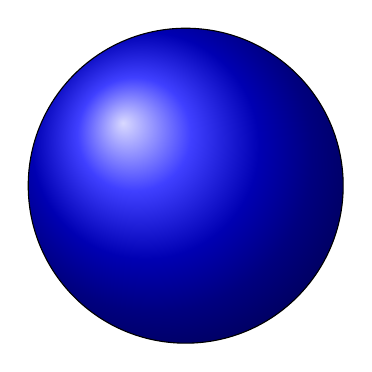
\begin{tikzpicture}
          \draw[shading = ball] (0, 0) circle (2);
    \end{tikzpicture}
\end{document}
    \caption[One ball]{One ball.}
\end{figure}

% Standalone with \includegraphics:
\begin{figure}[thbp]
    \centering
    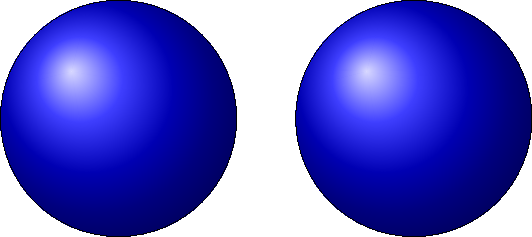
\includegraphics{balls}
    \caption[Two balls]{Two balls.}
\end{figure}

% Todonotes:
\begin{figure}[hbp]
    \centering
    \missingfigure{Three balls.}
    \caption[Three balls]{Three balls.}
\end{figure}

\kant[5-6] % Dummy text

% Booktabs:
\begin{table}[htbp]
    \centering
    \begin{tabular}{@{}ll@{}}
        \toprule
        \textbf{Correct}               & \textbf{Incorrect}      \\
        \midrule
        \( \varphi \colon X \to Y \)   & \( \varphi : X \to Y \) \\[0.5ex]
        \( \varphi(x) \coloneqq x^2 \) & \( \varphi(x) := x^2 \) \\
        \bottomrule
    \end{tabular}
    \caption[Colons]{Proper colon usage.}
\end{table}

\begin{table}[htbp]
    \centering
    \begin{tabular}{@{}ll@{}}
        \toprule
        \textbf{Correct}     & \textbf{Incorrect}         \\
        \midrule
        \( A \implies B \)   & \( A \Rightarrow B \)      \\
        \( A \impliedby B \) & \( A \Leftarrow B \)       \\
        \( A \iff B \)       & \( A \Leftrightarrow B \)  \\
        \bottomrule
    \end{tabular}
    \caption[Arrows]{Proper arrow usage.}
\end{table}

% Tablefootnote and multirow:
\begin{table}[htbp]
    \centering
    \begin{tabular}{@{}ll@{}}
        \toprule
        \textbf{Correct}
        & 
        \textbf{Incorrect}
        \\
        \midrule
        \( -1 \) 
        & 
        -1
        \\[0.3ex]
        1--10
        &
        1-10
        \\[0.3ex]
        Birch--Swinnerton-Dyer\tablefootnote{It is now easy to tell that Birch and Swinnerton-Dyer are two people.} conjecture
        &
        Birch-Swinnerton-Dyer conjecture
        \\[0.3ex]
        The ball \dash which is blue \dash is round.
        &
        \multirow{ 2}{*}{The ball - which is blue - is round.}
        \\[0.3ex]
        The ball---which is blue---is round. 
        &
        \\
        \bottomrule
    \end{tabular}
    \caption[Dashes]{Proper dash usage.}
\end{table}

\section{Outline}

The rest of the thesis is organised as follows:
\begin{description}
    \item[\cref{sec:second}]
    is second to none, with the notable exception of \cref{sec:intro}.
    The main tool introduced here is the employment of unintelligible sentences.
    
    \item[\cref{sec:third}]
    asserts the basic properties of being the third chapter of a thesis.
    This section reveals the shocking truth of filler content.
    
    \item[\cref{sec:fourth}]
    demonstrates how easily one can get to four chapters by simply using the \texttt{kantlipsum} package to generate dummy words.
    
    \item[\cref{sec:first-app}]
    features additional material for the specially interested.
    
    \item[\cref{sec:source}]
    consists of results best relegated to the back of the document,
    ensuring that nobody will ever read it.
\end{description}
    \chapter{Problem Description}
\label{sec:problem-description}

\section{The thesis problem description}

% TODO - insert the problem description given in the thesis announcement from FFI

    \chapter{Survey of Papers}

% \subsection{Related Work}

% http://msl.cs.uiuc.edu/~lavalle/cs497/jokane.pdf

% http://robotics.cs.unc.edu/BeliefSpacePlanning/index.html

\section{Survey}

Following is a survey of motion planning techniques incorporating uncertainty
with a focus on their application to unmanned ground vehicles (UGVs). First
described is the relevant sources of uncertainty in UGV motion planning, and
then the relevant techniques that have been applied to solve them in the
literature. In general uncertainty in UGV planning can be related to three
sources:
\begin{enumerate}
\item Uncertainty in  sensing.
\item Uncertainty in predictability.
\item Uncertainty in environment sensing.
\item Uncertainty in environment predictability.
\end{enumerate}~\cite{lavalleFrameworkMotionPlanning1995}

\subsection{Uncertainty in predictability}
Uncertainty in vehicle dynamics arises as the future robot configuration cannot
be predicted exactly. This results from modeling errors and/or limited precision
in the system's command tracking
performance~\cite{dadkhahSurveyMotionPlanning2012}. Thus a transfer from one
state to another will not guarantee full knowledge of the vehicle in the next
state. This is referred to as \textit{automated sequential decision making} in
the literature, and the mathematical framework used to tackle such uncertainty
is the \textit{Markov Decision Process} (MDPs), used to formulate an optimal
value problem, which then can be solved for an optimal value function, and the
corresponding optimal policy~\cite{Cassandra:1998:EAA:926710}. An introduction
to Markov decision processes can be found in \textit{grasping
  POMDs}\cite{kaelblingPlanningActingPartially1998}. This article uses apriori
known probability distributions in order to model uncertainty in the robot model
and in the sensors, then proceeds to use this to solve a number of different
objective functions. By focusing on the parts of space that are most likely to
be encountered, the problem is made tractable for real-life application. The
problem of solving POMDs lies with the size of the state space when this
solution strategy is applied to solving real-world problems - referred to as
\textit{the curse of dimensionality}. In fact
Tsilkis~\cite{christosh.papadimitriouComplexityMarkovDecision1987} showed that
solving such a problem is PSPACE-Complete and thus not tractable for real-life
applications. However approximate solutions are available, as shown by Kaelbling
et.\ al~\cite{kaelblingPlanningActingPartially1998}. Therefore the problem has
to be solved by using techniques such as sampling the belief space, as shown
in~\cite{kearnsSparseSamplingAlgorithm}. Another approach, using Monte-Carlo
simulation, is shown effective on large belief-spaces
in~\cite{silverMonteCarloPlanningLarge}.

% \subsubsection{Optimal Control Based Approaches}

\subsection{Uncertainty in Environment}
If the robot has imperfect or non-existent a-priori maps, or noisy sensory data,
complete deterministic knowledge of the environment is impossible. For an UGV in
an unknown environment, being able to have the situational awareness to avoid
collisions while adhering to the global planning requirements, despite
unpredicted obstacles appearing, is essential. Thus environment sensing and
mapping and re-planning in real-time is required. This is referred to in the
literature as planning in partially unknown environments. One solution to this
problem is through incremental graph-search algorithms, as shown
in~\cite{stentzOptimalEfficientPath}, where the \textsl{D*} algorithm is
described as a method for optimal and efficient re-planning in partially unknown
environments. Then \textit{Stentz}, a year later published the \textit{Focused
  D*} algorithm~\cite{stentz1995focussed}, which incorporates heuristics to
reduce the total time taken for re-planning. Still,\textit{D*} is
computationally heavy, and algorithms have been created to improve on the
time-bound of \textit{D*}. One such implementation is the \textit{D*-lite}
algorithm presented by Koenig~\cite{koenig2002d}. These incremental planners,
which incorporates the previously calculated plan in the solution of the newly
arisen planning problem speeds up the planning cycles, but can in many cases
still not be enough for a viable real-time solution. Finding a new plan within
the allotted planning interval may simply not be possible, in which case one can
resort to \textit{Anytime} algorithms, like Karaman et.\
al~\cite{karamanAnytimeMotionPlanning2011}, which will find an approximation in
the given time interval. Anytime planners find a solution quickly, and then
spends the rest of the allotted time on improving it until time runs out. One
such example of both an anytime and incremental solution is given
in~\cite{likhachevAnytimeSearchDynamic2008}. Another commonly used technique in
dealing with large state-spaces is sampling, and a popular approach to sampling,
is the \textit{Rapidly Exploring Random Tree} (RRT), which has shown itself
useful in dealing with high dimensional state-spaces. Several RRT-tweaks and
etensions have been proposed over the years, where a good comparison of
different versions of RRT (RRT*, RRT*-smart), can be found
in~\cite{noreenComparisonRRTRRT2016}. In order to deal with uncertainty, the
\textit{Particle-RRT} (pRRT) is proposed as an extension of the common RRT
algorithm into belief space, and then applied to a rover driving in rough
terrain~\cite{melchiorParticleRRTPath2007}. By propagating the uncertainty along
the planned path, and running this procedure multiple times, a cluster of nodes
is formed. Nodes in the search tree are then formed from these clusters, and a
likelihood can then be assigned to each path. Another RRT-extension is given
in~\cite{Luders_2013}, which present the \textit{Closed Loop Rapidly exploring
  Random Tree} (CC-RRT) algorithm, which can be employed for efficient
identification and execution of probabilistically safe paths in real-time in an
unknown and uncertain environment.


\subsubsection{Environment Mapping}
In the case that the map is only globally known, the local map may be wrong or
have errors, that the on-board local sensors will have to figure out. In order
to incorporate this into the planning procedure the field of mapping has to be
considered. In the literature this field is referred to as \textit{Simultaneous
  Location and Mapping} (SLAM). First of all virtually all robotic mapping
algorithms are probabilistic~\cite{thrunRoboticMappingSurvey}. % TODO - read
% this survey
A method which is called \textit{Occupancy Grid} is presented
in~\cite{elfes1989using}, in which the map is split up into cells, and each cell
is assigned a given probability of occupancy. It can incorporate information
from high-level maps using the same method that is used for estimating the
occupancy of a cell in a totally unknown environment. As the model is based on
Bayesian estimation, the initial map-data is used ad apriori input to the
probabilistic model. Thus the usage of a map of the area is voluntary. In this
way, unknown cells (those that are not yet inspected by local sensors) can be
assigned a high probability of occupancy. An old article on how this can be
implemented on a real robot is given by~\cite[Krugman]{kriegman1987mobile} More
recent work on the Occupancy Grid method can be found
in~\cite{carrilloAutonomousRoboticExploration2015}, which explores the trade-off
between exploring a new area, and relying on the information already obtained in
order to solve the problem. A method to integrate current map-data with the
on-board filter information is given in~\cite{gindeleBayesianOccupancyGrid2009}
using a Bayesian Occupancy Grid Filter for dynamic environments using prior map
knowledge.
\subsubsection{Integrating Planning and Mapping}
Not reasoning about the map and environment uncertainty can lead to crashes, as
further obstacles can be hidden behind other obstacles, and moving into
unexplored territory too fast will almost certainly lead to trouble. Thus using
a combination of sensing, mapping and re-planning is employed in part of the
literature on autonomous motion planning for UGVs. Using Chance constrained
programming as a solution to a problem modeled as a POMDP Vitus et.\
al~\cite{vitusHierarchicalMethodStochastic2012} shows that incorporating
real-time sensing into the model, which updates the probability a link in a
graph will be traversable depending on how well it has been sensed, then a
method is developed for balancing exploration and apriori knowledge of the
environment. The method is also employed experimentally on a quad-copter for
proof of real-time applicability. A method for assigning different probabilities
to different paths is given in~\cite{vandenbergLQGMPOptimizedPath2011} and is
based on the \textit{Linear Quadratic Gaussian Motion Planning} LQG-MP
algorithm. In~\cite{kurniawatiGlobalMotionPlanning2012} a motion planner called
\textit{Guided Cluster Sampling} is used to that takes into account all three
sources of uncertainty for robots with active sensing capabilities. This method
builds on the POMDP framework by utilizing a more suitable sampling distribution
based on the observations done by the robots active sensors.
In~\cite{yifenghuangRRTSLAMMotionPlanning2008} the \textit{RRT-SLAM} method is
introduced, where uncertainty is used in the RRT-planner by moving the state
space up a dimension, then this is joined together with a \textit{Simultaneous
  Location and Mapping} (SLAM) procedure. A ranking given on each path,
depending on its safety is given
in~\cite{blakeEfficientComputationCollision2018}.~\cite{bryRapidlyexploringRandomBelief2011}
gives an RRT algorithm that plans in belief space, and incorporates this with an
information region where the robot has little uncertainty, and can thus localize
itself. In case of adhering to the \textit{Plan Globally and Act Locally}
paradigm, a reactive planner coupled with a global path planner can provide a
complete navigation solution, as shown
in~\cite{djekouneSensorBasedNavigation2009}. This is useful in that a perfect
map of the environment may not be available. Worse even, the environment may
have changed, as nature is not static. Trees fall over, and floods move ground,
and create hindrances that might not be seen from a map. Not knowing where a
hindrance might lie, or whether one is located outside the sight of the onboard
sensors.

    \chapter{Preliminaries}
\label{chp:preliminaries}

Motion planning is the task of manipulating a robot's configurations so that,
given an initial and goal state or posture, the planner is able to create a
sequence of actions that gives a feasible or optimal path through the
overarching planning environment, usually referred to as the world space. Thus a
motion planner can be seen as a machine which given an input: a world, and
initial and goal states, produces a sequence of actions to move the robot from
its initial to the desired goal configuration. Generally, planners can be
separated into complete and non-complete planners, where being a complete
planner means that given enough time, all motion planning problems are solvable,
only the solution is NP-Hard, a non-complete planner makes no such
guarantees~\cite{Lav06}. Thus feasible solutions will have to make a compromise.
A lot of planners in use today are probabilistically complete, meaning that they
converge to a optimal solution given infinite time. There is a difference
between on-line and off-line motion planning, whereas the off-line algorithm
plans in a static environment, the online algorithm is run continuously. However
an on-line algorithm can be simulated by running an offline algorithm repeatedly
for short intervals of time. However, this comes with the drawback, that no
guarantee can be made for completing the task at hand \cite{Lav06}.

\section{The mathematical framework}

In order to build, model and reason about a motion planning problem, certain
nomenclature and definitions need to be standardized. A mathematical model of
the world, and the robot and its dynamics is necessary for clearly and precisely
reasoning about the problem at hand. Therefore the following sections creates
the mathematical definitions which is needed to create, understand and interpret
the following chapters.

\subsection{The Robot and World Model}

First of all the robot and the overarching motion planner needs a world in which
a plan is to be executed. In this thesis the world space is a 2-dimensional
plane, and is defined as:
\[
  \modelworld = \R^2
\]
In a real world planning problem not all parts of the world space is traversable
by the robot. As an example, in a forest, tree-trunks, branches, and other
inhabitants of the forest's vegetation will be untraversable for a robot, and
hence these obstacles needs to be modeled. As obstacles inhabit the world space,
they will be modeled as subsets of the world space, the same goes for the robot
body, which can be seen as yet another inhabitant of the world space.
\[
  \modelrobot,\, \modelobstacle \subset \modelworld
\]
Next the robot needs to be able to move around in the world space. This is done
through a rigid body transformation on the robot model
\[
  h : \modelrobot\ \rightarrow \modelworld
\]


\subsubsection{Configuration Space}

However, the robot is more than a set of points in the world space. For example
a simple model of an airplane needs to know its heading as well. This
information will be referred to as the configuration space of the robot
(\modelconfigurationspace). For a simple airplane model this can be encoded in a
simple three dimensional vector holding the \(x\), \(y\), and \(\theta\)
parameters, like so
\[
  \modelconfigurationspace \subset SE(2),
\]
which encompass all the states the robot can be in during planning. \(SE(2)\)
stands for \textit{Special Euclidean two}, and is defined as \(SE(2) = \R^2
\times \mathcal{S}\). As the robot lives in the world space, a subset of a
robot's configuration can be in collision with an obstacle.
\[
  \modelconfigurationspaceobst{} = \set{\vect{x} \in \modelconfigurationspace{} \mid
    \mathcal{A}(\vect{x}) \cap \modelobstacle{} \neq \emptyset}
\]
In the same way the free configuration space is defined as
\[
  \modelconfigurationspacefree{} = \mathcal{U} \setminus
  \modelconfigurationspaceobst{}
\]
where \(\mathcal{U}\) is the universe of the configuration space, meaning that
it is the union of \(\modelconfigurationspacefree \wedge
\modelconfigurationspaceobst\). More generally, the configuration space is a
model for a wide variety of motion planning problems. It is a manifold that
arise from the transformations applied to the robot. Thus in order to solve a
motion planning problem, a search must be performed in the configuration space.
Thus the motion planning problem is now made into a question of finding the best
path to traverse the given manifold created by the configuration space of the
robot~\cite{Lav06}.

\subsection{Action Space}

With the configuration space and robot motion in the world space defined, the
next problem is to control the movement of the robot model, which is where the
\textit{action space} comes in. The action space is the set of inputs that can
be applied at any given state the robot is in. Thus one can model the action
space as a function of the robot's state.
\[
  \modelactionspace(\x) = \set{\uin \in \modelactionspace \mid
    \modelactionspace(\x) \neq \emptyset }
\]

\subsection{Initial and Goal States}

A planning problem needs to have an initial condition, and a goal state or a set
of states in the configuration space. Since both the initial, and goal states
can be sets of states, it is not necessarily required to arrive exactly at the
target point. Rather it can arrive at some region close to it, while, for
example ignoring the final heading of the airplane. Mathematically the initial
and goal sets is defined as
\begin{align*}
  \mathcal{X}_0 &= \set{ \vect{x} \in \modelconfigurationspace{} \mid g_i(\vect{x}) \leq a_i,
                  \, \forall i = 1,\ldots N_j} \\
  \mathcal{X}_{end} &= \set{ \vect{x} \in \modelconfigurationspace{} \mid g_i(\vect{x}) \leq
                      a_i, \, \forall i = 1,\ldots N_k}
\end{align*}
which defines the initial and final states as subsets of the configuration space
bounded by inequality constraints, such that the initial and goal states are
semi-algebraic sets.

\subsection{Dynamics}

The model of the robot has so far been unconstrained and free to move in all
directions as it please under an affine transformation. This representation does
not encompass the dynamics a system might have, which constrains the direction
and speed in which a model can move. In the case of a first order model (i.e.,
it does not take accelerations into account) the constraints are represented as
a differential equation of the form:
\[
  \dot{\vect{x}} = f(\vect{x},\vect{u})
\]
where \(\vect{x}\) is the configuration, \(\vect{u}\) is the system input
control.

\subsection{Discrete motion planning}

As mentioned in the introduction, motion planning problems are in general
NP-hard. One way of making the problem more tractable is to discretisize the
problem. The discrete motion planning problem employs all the same definitions
as the continuous case for the world and robot model, only all points are
discrete in time \(t_k\) for some \(k\). Therefore, let \(\mathcal{X}\) be the
discrete state space, and \(\mathcal{U}(\vect{x}_k)\) be the set of actions
available at each point \(\vect{x}_k \in \mathcal{X}\). Then the state
transition equation can now written as:
\[
  \vect{x}_{k+1} = f(\vect{x}_k, \vect{u}_k)
\]

\subsubsection{Representation of the plan}

The plan that the motion planner makes for a robot in the configuration space is
represented as a trajectory. A trajectory is a path with an additional time
parameter, so that the path through configuration space is now time dependent.
This is represented as a function \(\phi(\alpha) \colon [0,1] \rightarrow
\mathcal{C}\), where \(\mathcal{C}\) is the configuration space of the airplane,
with the time parameter added the trajectory is represented as a
time-parameterized function of the kind \(\pi(t) \colon [0,T] \rightarrow
\mathcal{C}\), where \(T\) is the planning horizon (i.e., the end-time).

\subsection{Planning Under Uncertainty}

As all real life motion planning problems are faced with some level of
uncertainty the exact system state is never exactly known. Therefore planning
under uncertainty is done in what~\citeauthor{Lav06} refers to as the belief
space, which is a description of the state space using probability
distributions. The belief space is a general structure for working with plans
under conditions of uncertainty. Thus planning can be done mostly as it is done
in a normal state space, albeit in a higher dimension. If the discrete state
space model is expanded to include \(\mathcal{W}\) as the space of uncertain
actions, and \(\vect{w}_k\) is the action applied by an uncertain source at time
step \(k\), then the state transition transition is modeled as~\cite{Lav06}
\[
  \vect{x}_{k+1} = f(\vect{x}_k,\vect{u}_k,\vect{w}_k)
\]
As the uncertain actions are not available beforehand, that is -- \(\vect{w}_
k\) is not given, the model turns into
\[
  X_{k+1} = \set{ \vect{x}_{k+1} \in X \mid \exists w_k \in
    W(\vect{x}_k,\vect{u}_k) \text{ such that } \vect{x}_{k+1} =
    f(\vect{x}_k,\vect{u}_k,\vect{w}_k)}.
\] 

\subsection{Reachable sets}
\label{subsec:reachable-set}

Of particular interest to the \rrtfunnel{} algorithm is the reachable set. A
reachable set is all the configurations that the robot can be in if started from
a particular point in the configuration space. Had there been no constraints on
the movement of the robot the reachable set would simply be the entirety of the
configuration space. However, the simple unicycle model has both
\textit{kinodynamic} and \textit{non-holonomic} constraints. This leads to the
airplane not necessarily being able to reach all the states in the state-space
from a given starting point -- at least not given a time-frame. This idea is
important as it leads to the funnel definitions that makes up the backbone of
this thesis. As an example, the reachable set for the \textit{Dubins airplane}
(which is a simple airplane model, with a constant velocity and a control on the
heading of the airplane) is visualized in~\cref{fig:reachable-set-dubin}.

\begin{figure}
  \centering \documentclass[border=3mm,tikz]{standalone}
\begin{document}
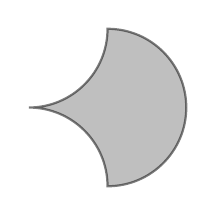
\begin{tikzpicture}
  \draw [black, fill=gray, opacity=.5, thick] (0,0) arc (270:360:1cm) -- (1,1) arc (90:-90:1cm)  -- (1,-1) arc (0:90:1cm);
\end{tikzpicture}
\end{document}
  \caption{The reachable set for a dubins car model after some time \(T\).}
  \label{fig:reachable-set-dubin}
\end{figure}

\subsection{Motion primitives}

The backbone of the \rrtfunnel{} algorithm is the composition of robust motion
primitives in order to construct a path from the initial, to the target
configuration. A motion primitive is a constant action applied over fixed time
interval. It is one or more actions collected into one discrete action. As an
example, the action the \textit{Dubin's airplane} employs is steering the angle
of the nose. Setting the angle to a constant over a time interval can be a
motion primitive, however, it is more easily thought of as a collection of
actions over time, which embodies one bigger, more abstract action. For the car
this could be \textit{go straight}, \textit{turn left}, etc. When composed
together, a collection of actions can be thought of as one simple action, like
first go straight and then turn left. The robustness signifies that it is robust
in the face of uncertainty, meaning that, if the uncertainty encountered is
within the bounds of the model, the motion primitives will be able accomplish
their task even in the face of this disturbance. This guarantee is developed in
the next section \cref{sec:funnels}.

\section{Funnels}
\label{sec:funnels}

The uncertainty guarantees in this thesis is made through creating
\textit{funnels}, which are the parameterization of the \textit{finite time
  reachable sets} for the dynamical system at hand. The following sections will
introduce and develop the theory needed in order to understand the \ac{SOS}
framework that lies at the bottom of the mathematical verification of these
reachable sets. For the curious reader, a more basic introduction can be found
in \cref{sec:first-app}.

A \textit{funnel} is a parameterization of the reachable set of a dynamical
system. This means that a Funnel holds all the states the dynamical system can
be in during a planning task. Mathematically the reachable set of the system is
defined as
\[
  \vect{x}(0) \in \mathcal{X}_0 \implies \vect{x}(t) \in F(t), \forall t \in
  \sqb{0,T}
\]
where \(\mathcal{X}_0\) is the set of initial conditions, \(\sqb{0,T}\) the time
interval, and \(F(t)\) is the set of states that the system can be in at time
\(t\). Although this thesis concerns itself with approximating the reachable set
through \textit{Lyapunov} functions, a useful analogy is imagining the funnel
created through \textit{Monte-Carlo} simulation, where the funnel would be the
set of all the paths traversed by the dynamical system at hand. For the simple
airplane model \cref{eq:model-dynamics}, a Monte-Carlo simulation of nine
starting points along the y-axis, along with a simple \ac{LQR} controller on the
heading of the aircraft, looks like~\cref{fig:monte-carlo-sim}.

\begin{figure}
  \centering 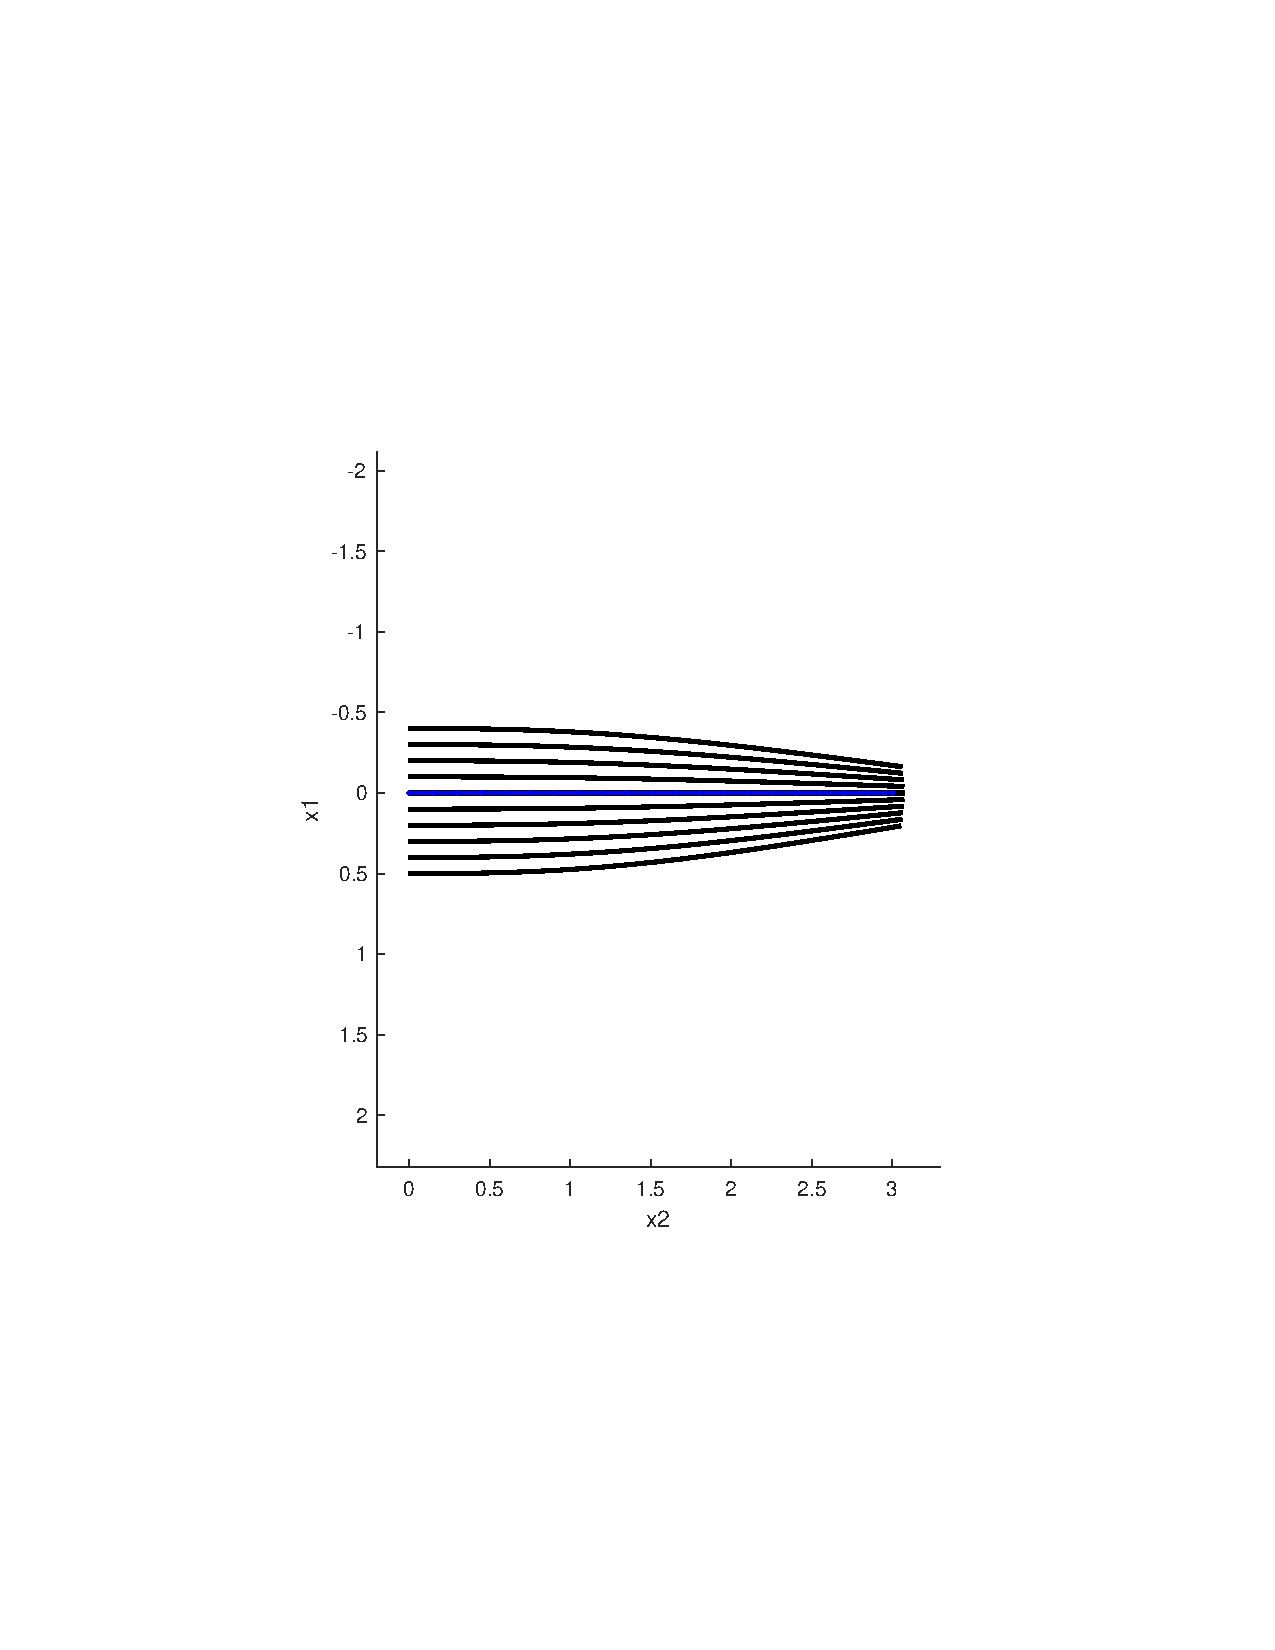
\includegraphics[scale=.5]{figures/preliminaries/montecarlofunnel}
  \caption{The simulation of N paths starting from a random point in the
    interval \(\sqb{-.5,.5}\), and controlled with a LQR controller.}
  \label{fig:monte-carlo-sim}
\end{figure}

In the literature, the term \textit{funnel} first appears in
\cite{masonMechanicsManipulation1985}, but is later employed in a lot of
research. The funnel definitions in this thesis is taken from a series of
articles on funnels \cite{Tobenkin_2011,tedrakeLQRtreesFeedbackMotion2009,
  majumdarRobustOnlineMotion2013,
  majumdarFunnelLibrariesRealtime2017,ahmadi2014dsos}, with the main focus being
on \cite{majumdarFunnelLibrariesRealtime2017}.

\subsection{Computing funnels}

The funnel computations will be based on the \ac{SOS} theory developed in the
following sections. Given a trajectory, the goal is to compute a robust
invariant set around the trajectory that will `guarantee' that the planner is
free from collisions during execution of the obtained motion plan. This robustly
invariant set is parameterized through Lyapunov function candidates, that, in
this case, will be based upon an \ac{LQR} controller for the system. The
following presentations is based on~\cite{Tobenkin_2011,
  tedrakeLQRtreesFeedbackMotion2009, majumdarRobustOnlineMotion2013}, but mainly
follow the formulations, and syntax
from~\cite{majumdarFunnelLibrariesRealtime2017}.

In order to compute funnels, a model of the dynamics for the system is required.
Thus, given the nonlinear dynamical system
\begin{equation}
  \label{eq:dynamicalsystem}
  \dot{\vect{x}} = f(\vect{x}(t), \vect{u}(t))
\end{equation}
with \(\vect{x}(t)\) the state of the system at time \(t\) and \(\vect{u}(t)\)
the control input. Assume that an open loop nominal trajectory \(\x_0 \colon
[0,T] \rightarrow \R^n\) with control input \(\vect{u}_0 \colon [0,T]
\rightarrow \R^n\) is given, and define a change of coordinates into the error
coordinate frame
\begin{align}
  \bar{\vect{x}}(t) &= (\vect{x} - \vect{x}_0)(t) \\
  \bar{\vect{u}}(t) &= (\vect{u} - \vect{u}_0)(t).
\end{align}
Then, transforming \cref{eq:dynamicalsystem} to the new coordinate frame one
obtains
\begin{equation}
  \label{eq:dynamicalsystem-coordinatechange}
  \dot{\bar{\vect{x}}} = \dot{\vect{x}} - \dot{\vect{x}}_0 = f(\vect{x}_0(t) + \bar{\vect{x}}(t), \vect{u}_0(t) + \bar{\vect{u}}(t)) - \dot{\vect{x}}_0(t)
\end{equation}

In order to compute a parameterized reachable set through \ac{SOS} programming
the system~\cref{eq:dynamicalsystem-coordinatechange} needs to be polynomial,
and parameterized by \(\vect{x}\) and \(t\) polynomially, since the \ac{SOS}
framework can only verify polynomials. Therefore, through the use of a
\ac{TV-LQR} controller (altough any controller providing a \ac{CLF} can be
used), the control input can be eliminated from the dynamical equation, giving
\begin{equation}
  \label{eq:dynamicclosedloop}
  \dot{\bar{\vect{x}}} = f_{cl}(t,\bar{\vect{x}}(t)).
\end{equation}
However, the dynamical system may still not be polynomial, which is a necessary
condition in order for this to be verified using \ac{SOS} programming.
Therefore, expanding the system~\cref{eq:dynamicclosedloop} around the nominal
trajectory \(\vect{x}_0\) is Taylor expanded to some degree high enough to
capture the nonlinearities of the system.

The goal is to parameterize a \textit{tight outer approximation} of the set of
states the system may transition into during the time interval \([0,T]\). Given
that \(F(t)\) is the set of states the system~\cref{eq:dynamicclosedloop} can be
in at time \(t\), then
\begin{equation}
  \label{eq:reachableset}
  \bar{\vect{x}}(0) \in \mathcal{X}_0 \implies \bar{\vect{x}}(t) \in F(t), \, \forall t \in [0,T]
\end{equation}
where \(\mathcal{X}_0\) is the initial condition set, and \(F(t) \subset \R^n\)
is the finite time funnel for the system.

A funnel is defined by \citeauthor{majumdarFunnelLibrariesRealtime2017} in
\cite{majumdarFunnelLibrariesRealtime2017} as
\begin{definition}
  \label{def:funnel}
  A funnel associated with a closed-loop dynamical system
  \(\dot{\bar{\vect{x}}} = f_{cl}(t,\vect{x}(t))\) is a map \(F \colon [0,T]
  \rightarrow \mathcal{P}(\R^n)\), from the time interval \([0,T]\) to the power
  set (i.e., the set of subsets) of \(\R^n\) so that the sets \(F(t)\) satisfy
  the condition~\cref{eq:reachableset}.
\end{definition}

Next, the reachable set is parameterized through the use of Lyapunov functions,
which yields
\begin{equation}
  F(t) = \set{\bar{\vect{x}}(t) \mid V(t, \bar{\vect{x}}(t) \leq \rho (t))}
\end{equation}
where \(\rho (t) \colon [0,T] \rightarrow \R^+\), is a function which limits the
size of the reachable set, and \(V(t,\bar{x}(t))\) is a Lyapunov function \(V
\colon [0,T] \times \R^n \rightarrow \R^+\).

Then, by setting \(\mathcal{X}_0 \subset F(0,\bar{\vect{x}})\), one can derive
the sufficient condition~\cref{eq:reachableset} for containing the reachable set
in the Lyapunov function parameterization
\begin{equation}
  \label{eq:funnelsufficient}
  V(t,\bar{\vect{x}}) = \rho(t) \implies \dot{V}(t,\bar{\vect{x}}) < \dot{\rho}(t), \, \forall t \in [0,T]
\end{equation}
with \(\dot{V}(t,\bar{\vect{x}})\) computed as
\begin{equation}
  \dot{V}(t,\bar{\vect{x}}) = \frac{\partial V(t,\bar{\vect{x}})}{\partial \vect{x}} f_{cl}(t,\bar{\vect{x}}) + \frac{\partial V(t,\bar{\vect{x}})}{\partial t}
\end{equation}

Currently there are no limitations on the functions \(V\) and \(\rho\), and
hence there exists infinitely many functions with different sized reachable sets
that satisfies~\cref{eq:funnelsufficient}, and is a valid funnel in the sense of
~\cref{def:funnel}. In order for efficient planning to take place, the motion
primitives, meaning the size of the funnels, should be as small as possible, and
it is therefore that the size of the funnels is minimized using the following
optimization problem~\cite{majumdarFunnelLibrariesRealtime2017}

\begin{align}
  \label{eq:funneloptimizationproblem}
  &\underset{V,\rho}{\text{inf}} \; &&\int_{0}^{T} \vol(F(t))\, dt \\
  &\text{subject to} && V(t,\bar{\vect{x}}) = \rho (t) \implies \dot{V}(t,\bar{\vect{x}}) < \rho (t) \, \forall t \in [0,T] \nonumber \\
  && &\mathcal{X}_0 \subset F(0,\bar{\vect{x}}) \nonumber
\end{align} 

\begin{figure}
  \centering
  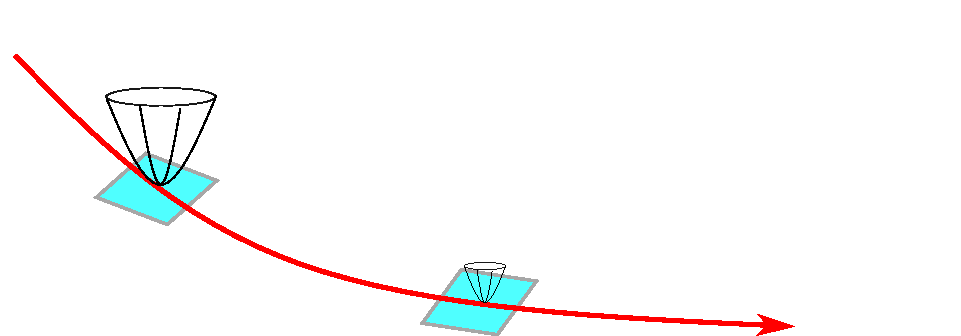
\includegraphics[scale=.7]{figures/experiments/lyapunov_visualization}
  \caption{A visualization of the Lyapunov function along a trajectory, where
    the center of the Lyapunov function moves along the trajectory with time
    \(t\).}
\end{figure}


\subsection{Formulating the optimization problem as a SOS program}

The optimization problem in~\cref{eq:funneloptimizationproblem} would prove
impossible to solve efficiently had it not been for advances in mathematical
convex numerical optimization by
\citeauthor{parilloStructuredSemidefinitePrograms}~\cite{parilloStructuredSemidefinitePrograms},
as in general the problem involves searching over an infinite function space.
While the general optimization problem of searching through the infinite
function space is not amenable to efficient numerical computation, the problem
can be made computationally feasible through the use of a \ac{SOS} programming
approach~\cite{tedrakeLQRtreesFeedbackMotion2009}.

Thus in order to make the problem amenable to a \ac{SOS} program, there are a
few requirements that needs to be met by the problem formulation. Firstly the
initial condition set needs to be a \textit{semi-algebraic set}, (i.e.,
parameterized by polynomial inequalities),
%
\begin{equation}
  \mathcal{X}_0 = \set{\bar{\vect{x}} \in \R^n \mid g_{o,i}(\bar{\vect{x}}) \geq 0, \, i = 1,\ldots,N_0}
\end{equation}
%
then rewriting~\cref{eq:funneloptimizationproblem}~as in terms of positivity and
equality constraints yields
\begin{equation}
  V(t,\bar{\vect{x}}) = \rho(t) \implies \dot{\rho}(t) - \dot{V}(t,\bar{\vect{x}}) > 0
\end{equation}
and
\begin{equation}
  g_{0,i}(\bar{\vect{x}}) \geq 0 \, \forall i \in \set{1,\ldots,N_0} \implies \rho(0) - V(0,\bar{\vect{x}}) \geq 0
\end{equation}
which, if these functions are both polynomial, is now in the form of a \ac{SOS}
optimization problem. Then through the use of the~\nameref{sec:s-procedure} one
arrives at the equations
\begin{align}
  &\dot{\rho}(t) - \dot{V}(t,\bar{\vect{x}}) - L(t,\bar{\vect{x}})\left( V(t,\bar{\vect{x}}) - \rho(t) \right) - L_{t}(t,\bar{\vect{x}})\left( t\left( T - t \right) \right)  && \text{is SOS}& \label{eq:sufficient-conditions}\\
  & \rho(0) - V(0,\bar{\vect{x}}) - \sum_{i}^{N_{0}} L_{0,i}(\bar{\vect{x}})g_{0,i}(\bar{\vect{x}}) && \text{is SOS}& \nonumber \\
  & L(t, \bar{\vect{x}}), \, L_{t}(\bar{\vect{x}}), \, L_{0,i}(\bar{\vect{x}}) \; &&\text{are SOS}, \, \forall i \in \set{1,\ldots,N_{0}} \nonumber
\end{align} 
where \(L\), \(L_{t}\), and \(L_{0,i}\) are multiplier polynomials~(see
\labelcref{sec:s-procedure}).

The goal is to make the parameterization of the reachable set as small as
possible, and therefore minimizing the cost
function~\cref{eq:funneloptimizationproblem}. This is done by
\citeauthor{Tobenkin_2011} in~\cite{Tobenkin_2011}, through approximating the
cost function by first discretizing the problem and replacing the integral with
a finite sum
\begin{equation}
  \int_{0}^{T} \vol(F(t))\, \mathrm{d}t \rightarrow \sum_{k=1}^{N} \vol(F(t_{k})) \label{eq:discrete-costfunction}.
\end{equation}
Since the Lyapunov function \(V(t,\bar{\vect{x}})\) in this thesis is quadratic,
it can be written as
\begin{equation}
  V(t_{k}, \bar{\vect{x}}) = {\bar{\vect{x}}}^{T}S_{k}\bar{\vect{x}}, \, S_{k} \succeq 0
\end{equation}
which means that the set \(F(t_{k})\) is an ellipsoid in which the volume can be
minimized through maximizing the determinant of \(S_{k}\), which in turn can be
transformed into a \ac{SDP} problem. If an upper bound on the cost
function~\cref{eq:discrete-costfunction} is introduced as
\begin{equation}
  \mathcal{E} (t_{k}) = \set{\bar{\vect{x}} \in \R^n \mid {\bar{\vect{x}}}^{T}S_{k}\bar{\vect{x}} \leq 1, \, S_{k} \succeq 0}
\end{equation}
where \( \mathcal{E} ( t_{k} ) \) is an ellipsoid containing the reachable set
\( F ( t_{k} ) \) at time \( t_{k} \). This containment constraint can be
equivalently expressed as
\begin{equation}
  V ( t_{k}, \bar{\vect{x}} ) \leq \rho(t_{k})  \implies {\bar{\vect{x}}}^{T}\matr{S}_{k}\bar{\vect{x}} \leq 1.
  \label{eq:discrete-containment-constraint}
\end{equation}
Which when expressed using \ac{SOS} constraints gives
\begin{align}
  1 - {\bar{\vect{x}}}^{T}\matr{S}_{k}\bar{\vect{x}} - L_{\mathcal{E},k}(\bar{\vect{x}})\left( \rho(t_{k}) - V(t_{k}, \bar{\vect{x}}) \right)  \qquad \text{is SOS}& \\
  L_{\mathcal{E},k}(\bar{\vect{x}}) \qquad \text{is SOS.}& \nonumber
\end{align}
%
Then combining the cost function~\cref{eq:discrete-costfunction} with the
constraints~\cref{eq:discrete-containment-constraint}, one arrives at the
optimization problem
%
{ % Mini environment scope
  \newcommand{\E}{\mathcal{E}} \renewcommand{\x}{\bar{x}}
  \begin{mini*}[1]
    { \substack { V, \rho, L, L_t,
        \\
        L_{0, i}, S_{k}, L_{\E, k} } } { \sum_{k = 1}^{N} \vol(\E(t_{k})) =
      \sum_{k = 1}^{N} \vol \p{\set{\vect{x} \mid \vect{x}^T \matr{S}_k \vect{x}
          \le 1}} } {} {} \addConstraint { \dot{\rho}(t) -
      \dot{V}(t,\vect{x}) - L(t,\vect{x}) \sqb*{ V(t,\vect{x}) - \rho(t) } - L_t
      (t,\vect{x}) \sqb*{t \p*{T - t}} }%
    {\text{ is SOS}} \addConstraint {\rho(0) - V(0, \vect{x}) - \sum_i^N L_{0,
        i}(\vect{x}) g_{0, i}(\x)}%
    {\text{ is SOS}} \addConstraint { 1 - \vect{x}^T \matr{S}_k \vect{x} -
      L_{\E, k}(\vect{x}) \sqb*{\rho(t_k) - V(t_k, \vect{x})} }%
    {\text{ is SOS}} \addConstraint {S_k}%
    {\succeq 0}%
    {\quad \forall k \in \set{1, \ldots, N}} \addConstraint {L_t (t,
      \vect{x}),\, L_{0,i}(\vect{x})}%
    {\text{ are SOS}}%
    {\quad \forall i \in \set{1, \ldots, N_0}} \addConstraint{}{}{\quad \forall
      k \in \set{1, \ldots, N}.}
  \end{mini*}
} % End optimization problem scope.
which is the finite dimensional optimization problem needed in order to search
for a Lyapunov function candidate.

However, this optimization problem is not convex in general, as the first
constraints are \textit{bilinear} in the decision variables, since \(L\) and
\(V\) are multiplied together. However, the problem can be solved, although not
optimally, if \(V\) and \(\rho\) are held fixed, while the other decision
variables are free. Likewise, fixing \(L\) and \(L_{\mathcal{E},k}\), creates
another \ac{SOS} optimization program. Therefore shifting between the two sets
of decision variables
\[
  \left( L,L_{t},L_{0,i},L_{\mathcal{E},k} \right)
\]
and
\[
  \left( V,\rho,L_{0,i},\matr{S}_{k} \right)
\]
\citeauthor{majumdarFunnelLibrariesRealtime2017}~\cite{majumdarFunnelLibrariesRealtime2017}
arrives at the \cref{alg:funnelalgorithm} for funnel computation:

\begin{algorithm}
  \caption{Funnel computation}
  \label{alg:funnelalgorithm}
  \DontPrintSemicolon \SetAlgoNoLine

  \KwIn{\(V\) and \(\rho\)} \KwOut{Funnel}

  \(cost_{prev} = \infty\)\; converged = false \; \While{\(!\; converged\)}{
    Optimization problem 1: \;
    \begin{align*}
      \underset{\substack{L,L_{t},L_{0,i},S_{k},L_{}}}{\inf}&  \sum_{k=1}^{N} \vol(\mathcal{E}(t_{k}))& \\    
      \text{subject to } & V \text{ and } \rho \text{ constant.}& \\
    \end{align*}\;
    Optimization problem 2: \;
    \begin{align*}
      \underset{\substack{V,\rho, L_{t},L_{0,i},S_{k}}}{\inf}&  \sum_{k=1}^{N} \vol(\mathcal{E}(t_{k}))& \\    
      \text{subject to } & L \text{ and } L_{\mathcal{E},k} \text{ constant.}& \\
    \end{align*}\;
    cost = \(\sum_{k=1}^{N} \vol(\mathcal{E}(t_{k}))\) \;
    \If{\(\frac{cost_{prev} - cost}{cost_{prev}} < \epsilon\)} {
      converged = true
    }\;
    \(cost_{prev} = cost\)\;
  }\;
\end{algorithm}

\subsection{Approximation via time-sampling}

It is often the case that the nominal trajectory \(x_{0} \colon [0,T]
\rightarrow \R^n\) is difficult to approximate with a low degree polynomial in
time~\cite{majumdarFunnelLibrariesRealtime2017}. As this can cause funnel
computation to take a lot of time, approximating the polynomial discretely
helps, but exactness will be lost, however the resulting funnels are shown to be
acceptable approximations, where exactness can be regained through increasing
the sampling rate~\cite{Tobenkin_2011}. If \(t_{k} \in [0,T]\), where \(k \in
\set{1,\ldots,N}\), the optimization equations become:

\begin{mini}
  {\substack{V_{k}, \rho, L_{k},\\ L_{0,i}, S_{k},
      L_{\mathcal{E},k}}} % Optimization variables
  {\sum_{k=1}^{N}\vol(\mathcal{E}(t_{k})) = \sum_{k=1}^{N} \vol\left(
      \set{\bar{x} \mid {\bar{x}}^{T} S_{k} \bar{x} \leq 1}
    \right)} % Optimization function
  {\label{optidef:discrete}} % Label optimization problem
  {} % Optimization result
  % Constraints
  \addConstraint{\dot{\rho}(t_{k}) - \dot{V}_{k}(\bar{\vect{x}}) -
    L_{k}(\bar{\vect{x}}) \left( V_{k}(\bar{\vect{x}}) - \rho(t_{k}) \right)}
  {\qquad} {\forall k \in \set{1,\ldots,N}} \addConstraint{\rho(t_{1}) -
    V_{1}(\bar{\vect{x}}) - \sum_{i}^{N_{0}} L_{0,i}g_{0,i}(\bar{\vect{x}})} {\,
    \text{is SOS}} {} %
  \addConstraint{1 - {\bar{\vect{x}}}^{T} S_{k} \bar{\vect{x}} -
    L_{\mathcal{E,k}} \left( \rho(t_{k}) - V_{k}(\bar{\vect{x}}) \right)} {\,
    \text{is SOS}\;} {\forall k \in \set{1,\ldots,N}} %
  \addConstraint{S_{k} \succeq 0} {} {\forall k \in \set{1,\ldots,N}} %
  \addConstraint{L_k(\bar{\vect{x}}),\,L_{0,i}(\bar{\vect{x}}), L_{\mathcal{E},k}} {\, \text{are SOS}}
  {\; \forall i,k \in \set{1,\ldots,N}} %
\end{mini}

\subsection{Funnel composition}

In order for two funnels being able to together create one longer motion
primitive, from two or more smaller, the funnels in use must be composable. In
order for two \funnel's to be composable, the outlet of one \funnel{} needs to
be completely contained within the inlet of the other. This means that if
\(\mathcal{F}_1 = F_1(T)\) is the outlet of \funnel{} \(F_1\), and
\(\mathcal{F}_2 = F_2(0)\) is the inlet of \(F_2\), then
\begin{equation}
  \label{eq:funnel-subset}
  \mathcal{F}_1 \subseteq \mathcal{F}_2
\end{equation}
is required in order for the funnels to be composable. In
\citeauthor{majumdarFunnelLibrariesRealtime2017}~\cite[47]{majumdarFunnelLibrariesRealtime2017},
two funnels are sequentially composable if
\begin{definition}
  \label{def:funnel-composition}
  An ordered pair \((F1, F2)\) of funnels \(F_1 \colon [0,T_1] \rightarrow
  \mathcal{P}(\R^n)\) and \(F_2 \colon [0,T_2] \rightarrow \mathcal{P}(\R^n)\)
  is sequentially composable if \(F_1(T) \subseteq F_2(0)\).
\end{definition}
Thus
\begin{equation}
  V_1(T_1,\bar{\vect{x}}) \leq \rho_1(T_1) \implies V_2(0,\bar{\vect{x}}) \leq
  \rho_2(0)
\end{equation}
is an equivalent condition to~\cref{eq:funnel-subset}, and which can be checked
through the following \ac{SOS} program
\begin{align*}
  \text{Find } \; &L(\bar{x}) \\
  \text{s.t} \; &\rho_2(0) - V_2(0,\bar{\vect{x}}) - L(\bar{\vect{x}})
                  \left( \rho_1(T_1) - V_1(T_1,\bar{\vect{x}}) \right).
\end{align*}

However in
\citeauthor{majumdarFunnelLibrariesRealtime2017}~\cite{majumdarFunnelLibrariesRealtime2017},
the program is simply stated, and it can be helpful to take a look at the
derivation in order to gain a feel of the implementation of a \ac{SOS} program.

The \nameref{sec:s-procedure} enables us to limit our search to a semi-algebraic
set. In this case, that set is \(\mathcal{F}_2 = \set{\vect{x} \in \R^n \mid
  V_2(0,\bar{\vect{x}}) \leq \rho_2(0)}\), any \(\vect{x}\) that is not in this
set does not concern us, which is why employing the \textit{S-Procedure} is
valid. In more general terms this can be written
\[
  \vect{x} \in \mathcal{F}_2 \implies p(\vect{x}) \geq 0
\]
where \(p(\vect{x})\) is the \ac{SOS} polynomial that is to be verified. In this
case \(p(\vect{x})\) is \(V_2(0,\bar{\vect{x}})\). Thus in order to impose the
implication define
\[
  q(\vect{x}) = V_2(0,\bar{\vect{x}}) - \rho_2(0) - L(\bar{\vect{x}}) \left(
    \rho_1(T_1) - V_1(T_1,\bar{\vect{x}}) \right)
\]
where \(q(\vect{x})\) and \(L(\bar{\vect{x}})\) needs to be SOS polynomials.

\begin{example}

  As a simple example let's have a look at embedding a square within a circle.
  For good measure let's give the circle a radius of \(\sqrt{2}+\epsilon\), and
  the square a radius of \(1\), and center them both at the origin in the
  Euclidean plane.

  Starting with defining the set \(\beta\)
  \[
    \beta = \set{\vect{x} \in \R^2 \mid \norm{\vect{x}} \leq 1}
  \]
  using the Manhattan metric. then the implication
  \[
    \vect{x} \in \beta \implies p(\vect{x}) \geq 0
  \]
  which can be formulated as
  \begin{align*}
    \beta &= \set{\vect{x} \in \R^2 \mid 1 \pm \vect{x} \geq 0 } \\
    p(\vect{x}) &= r^2 - x^2 - y^2
  \end{align*}
  where \(p(\vect{x})\) is the parameterization of the circle, and \(\beta\) is
  the parameterization of the square with sides of length two. What needs to be
  shown is that \(p(x)\) is positive on the set \(\beta\). Through the
  \nameref{sec:s-procedure} this can be written as the search for a nonnegative
  polynomial \(L_{ineq,i}(\vect{x})\) such that \(p(\vect{x}) \geq
  L_{ineq,i}(\vect{x})g(\vect{x}) \). Thus
  \[
    q(\vect{x}) = p(\vect{x}) -
    \sum_{i=1}^{2}L_{ineq,i}(\vect{x})g_{ineq,i}(\vect{x})
  \]
  is required to be a \ac{SOS} polynomial, along with \(L_{ineq,i}\). From this
  it is seen that when a point satisfies \(g_{ineq,i}\) (i.e., when \(\vect{x} \in
  \beta\)) the term \( - \sum_{i=1}^{2}L_{ineq,i}(\vect{x})g_{ineq,i}(\vect{x})\)
  is negative, and hence \(p(x)\) must be nonnegative, which gives the desired
  implication.

  Solving this problem can be done using any of a number of \ac{SOS} modeling
  software. This example will rely on \textsc{Yalmip}~\cite{Lofberg2004} and its
  \ac{SOS} programming functionality \cite{Lofberg2009} for \matlab.


  \lstinputlisting{figures/funnel/embededsquare.m}

  Which returns ``Composition successful!'' for circles with radii larger than
  \(\sqrt{2}\) as expected.
\end{example}

\subsection{Cyclic coordinates and Lagrangian dynamics}
\label{subsec:cyclic-coordinates}

In order to move funnels around the world space, the dynamics of the system must
not change along the coordinates at which the system is manipulated. This can be
achieved through the theory of cyclic and non-cyclic coordinates, stemming from
the Lagrangian dynamics of the system. Therefore, given the Lagrangian
\(\mathcal{L}(q_i, \dot{q_i}, t)\) of a dynamical system, where the \(q_i\) are
the generalized coordinates of the system, and \(\dot{q_i}\) are the
generalized velocities. If the Lagrangian does not contain the \(q_j\) then
\(q_j\) is a cyclic coordinate of the system, and the j-th Lagrangian has the
form
\[
  \left( \frac{d}{dt} \right) \left( \frac{\partial \mathcal{L}}{\partial
      \dot{q_j}} \right) = \mathrm{const}
\]
This means that any \(q_j\) fulfilling the above criteria can be freely moved
around in the state-space, yet yield the same dynamical solution of the system.



    % \chapter{RRT}

The planning algorithm used in this thesis will build upon the \textit{Rapidly
  Exploring Tree} algorithm, which was first proposed by LaValle and . in TODO
\cite{TODO}.

\begin{figure}
  \centering
  \begin{subfigure}[b]{0.3\textwidth}
    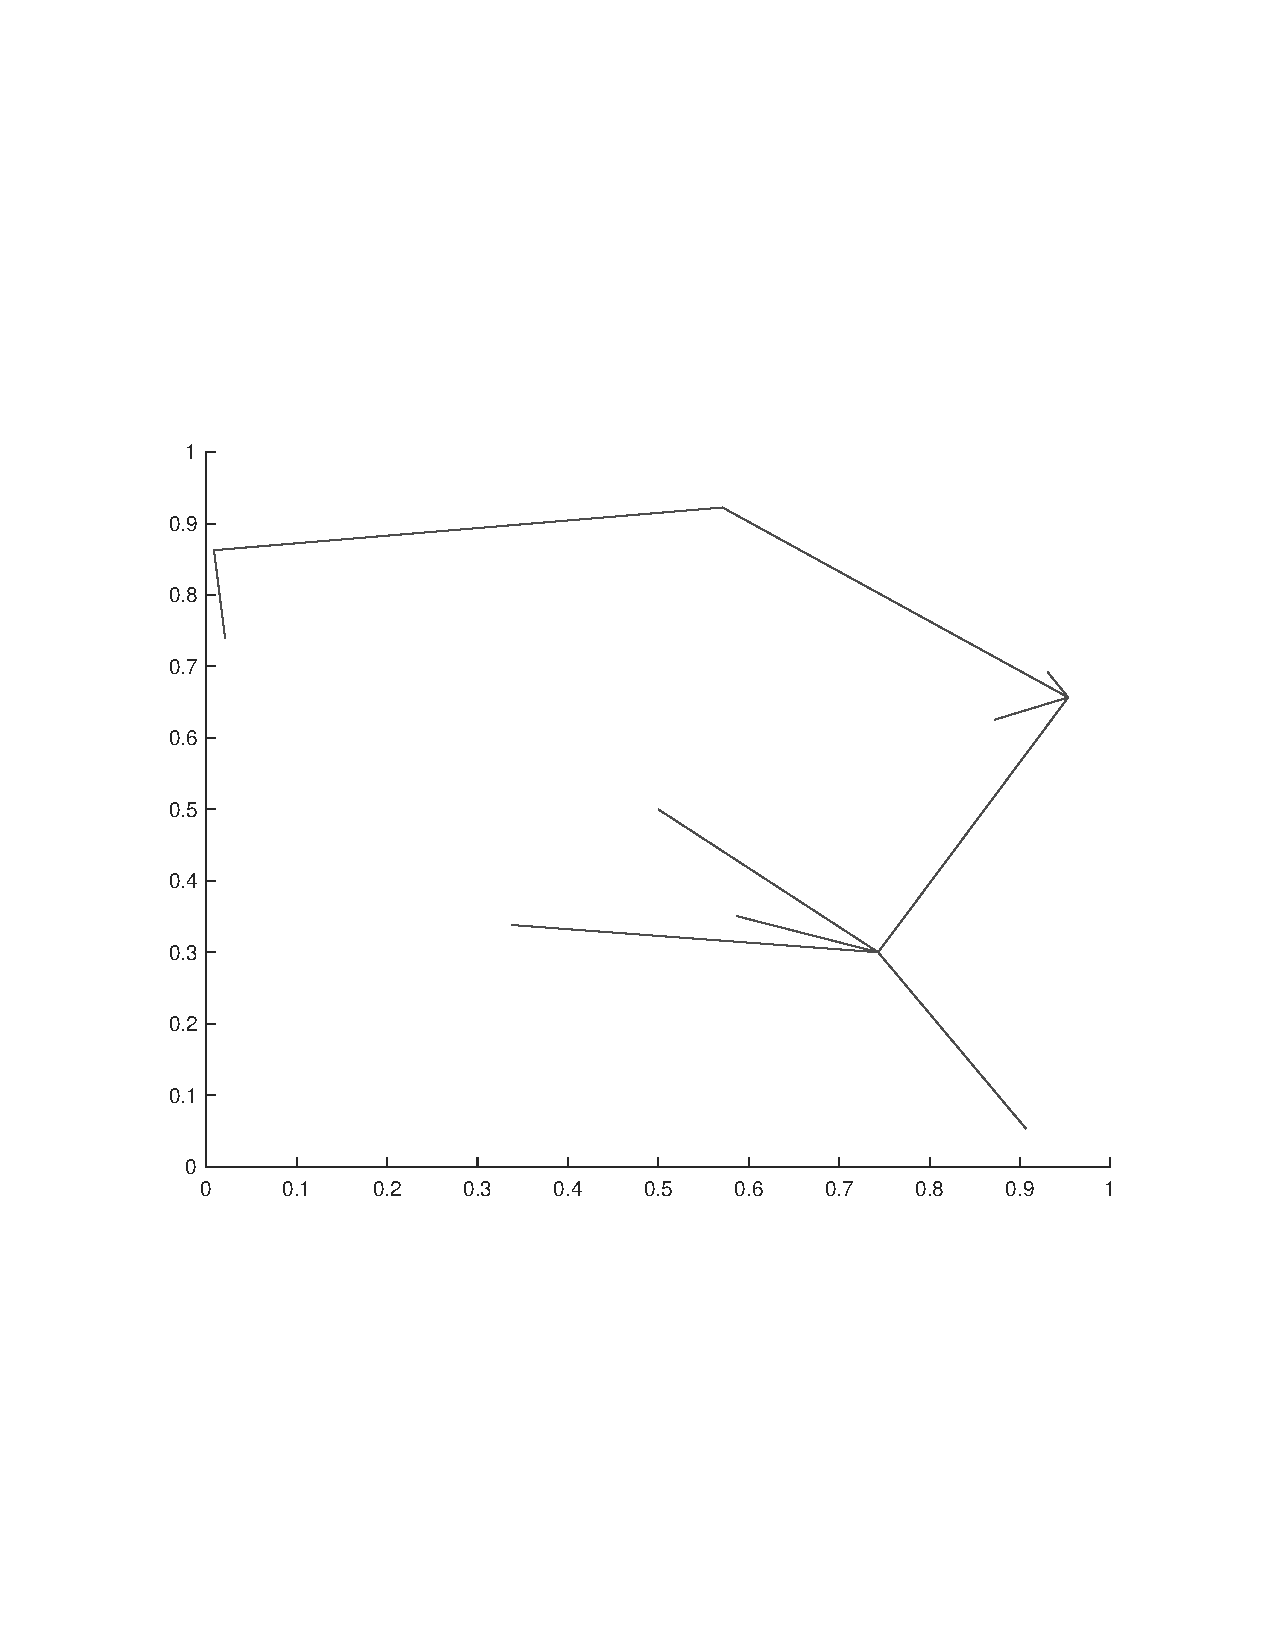
\includegraphics[width=\textwidth]{plainRRT10}
    \caption{RRT-tree after 10 iterations.}
  \end{subfigure}
  \begin{subfigure}[b]{0.3\textwidth}
    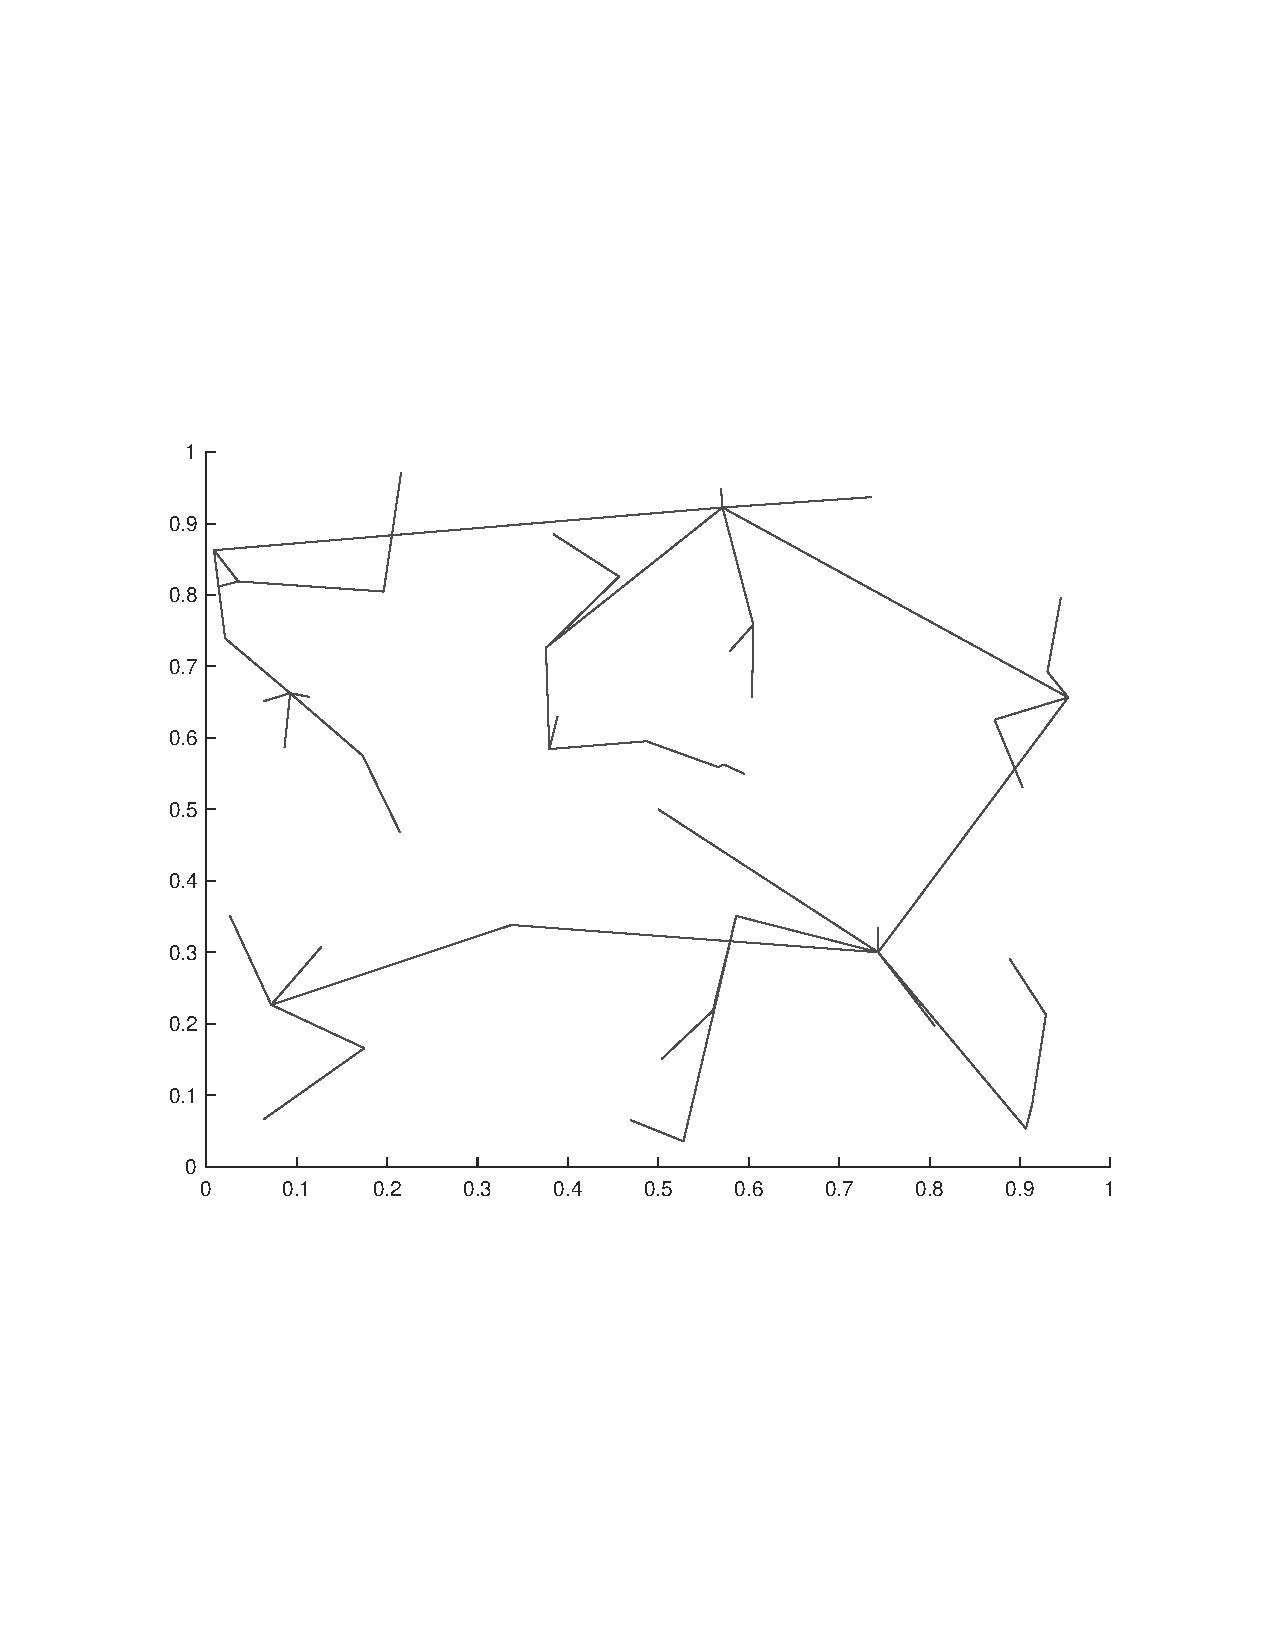
\includegraphics[width=\textwidth]{plainRRT50}
    \caption{RRT-tree after 50 iterations.}
  \end{subfigure}
  \begin{subfigure}[b]{0.3\textwidth}
    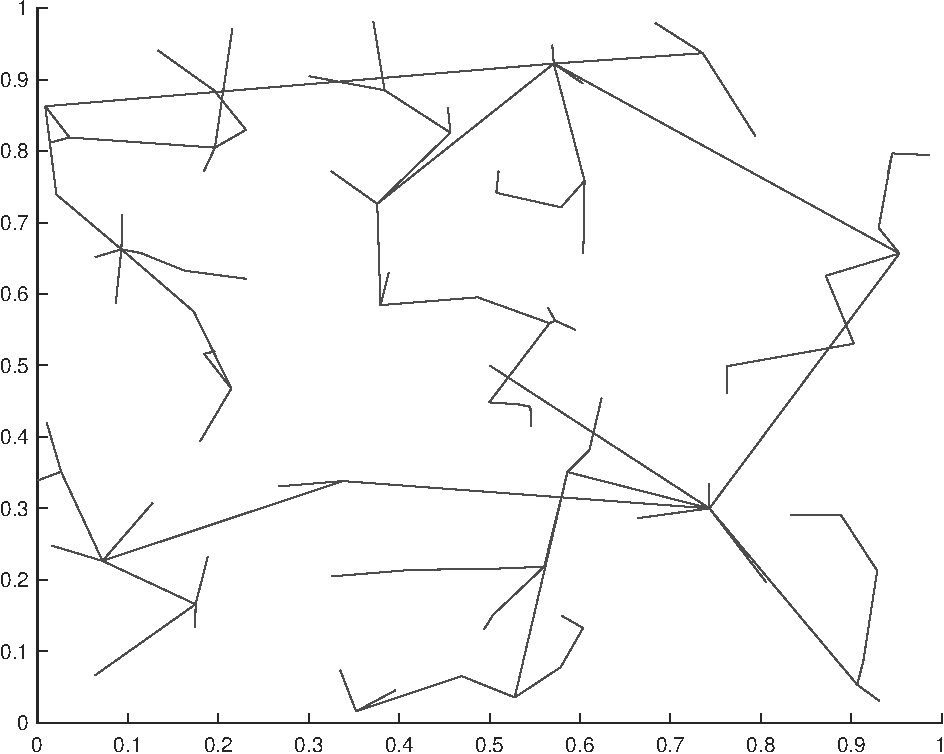
\includegraphics[width=\textwidth]{plainRRT100}
    \caption{RRT-tree after 100 iterations.}
  \end{subfigure}
  \newline % Start the new line of plainRRT10.
  \begin{subfigure}[b]{0.3\textwidth}
    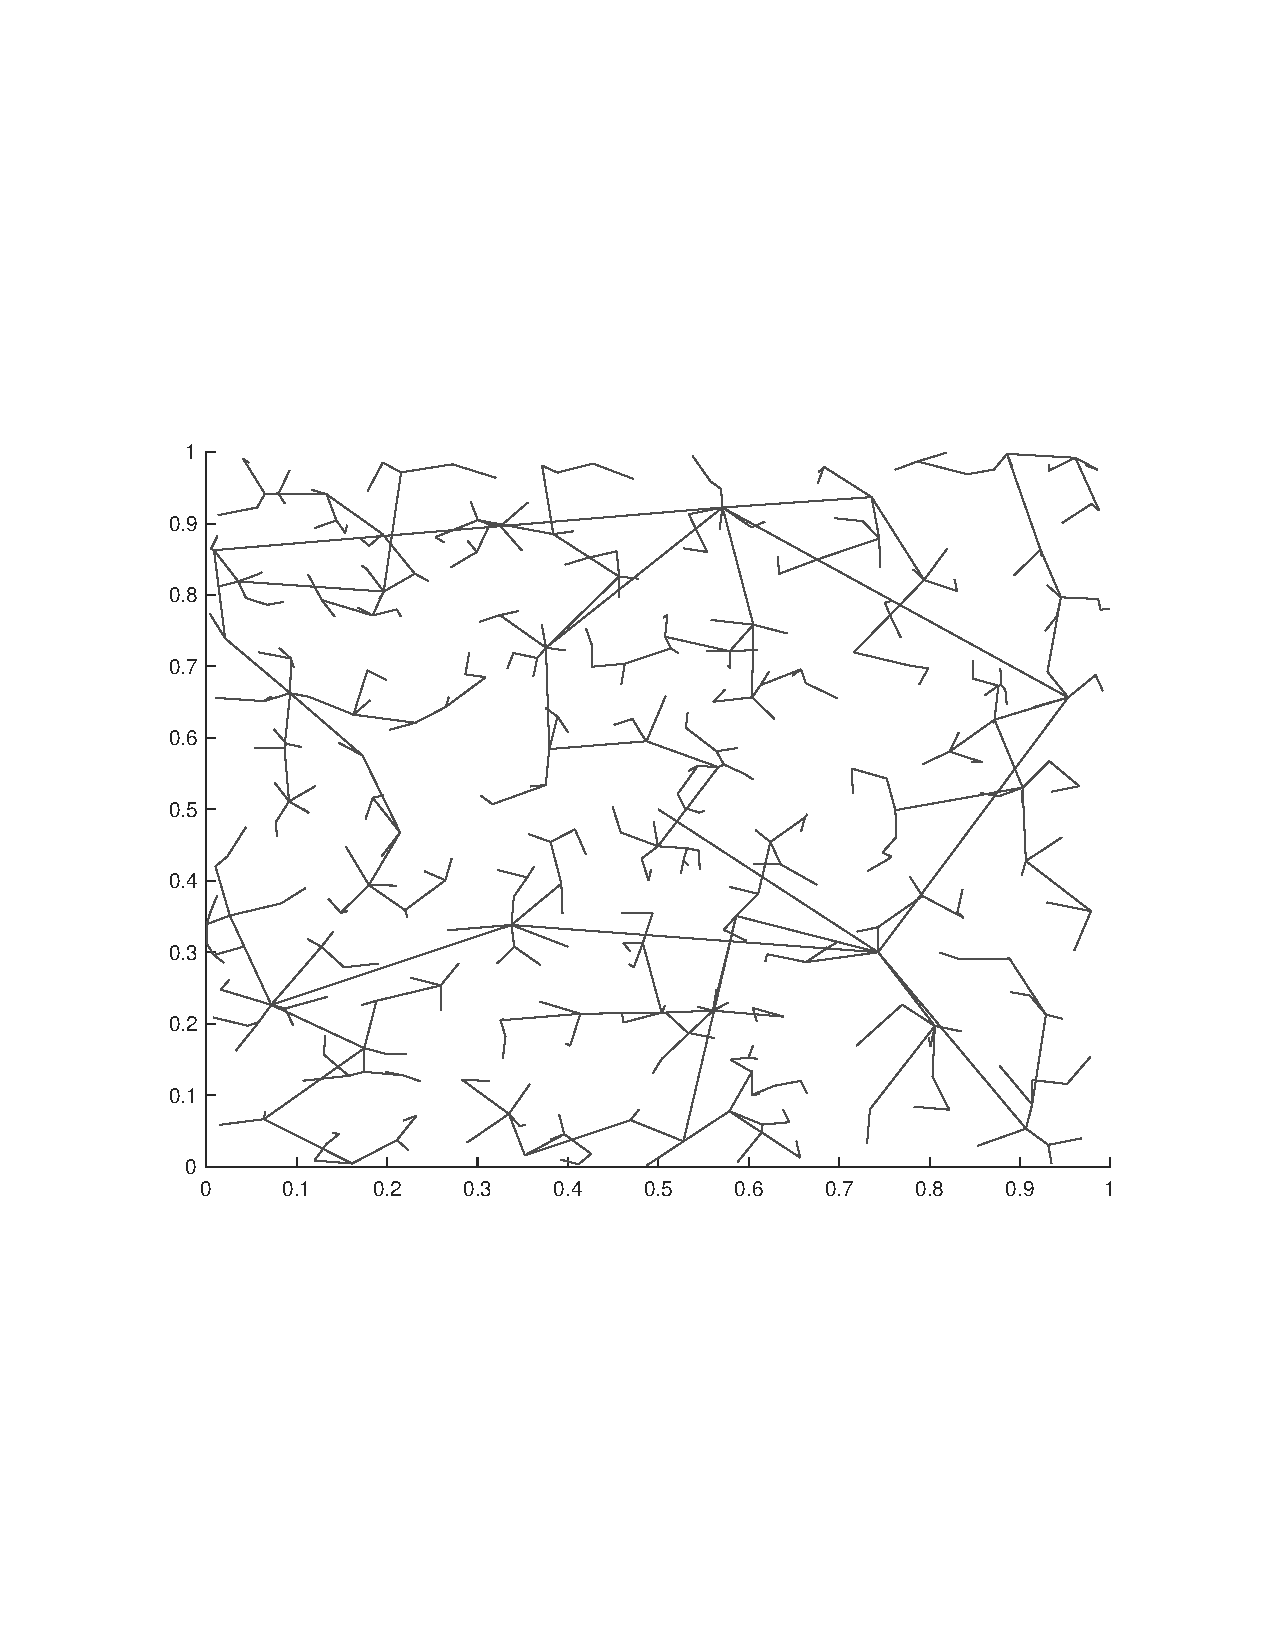
\includegraphics[width=\textwidth]{plainRRT500}
    \caption{RRT-tree after 500 iterations.}
  \end{subfigure}
  \begin{subfigure}[b]{0.3\textwidth}
    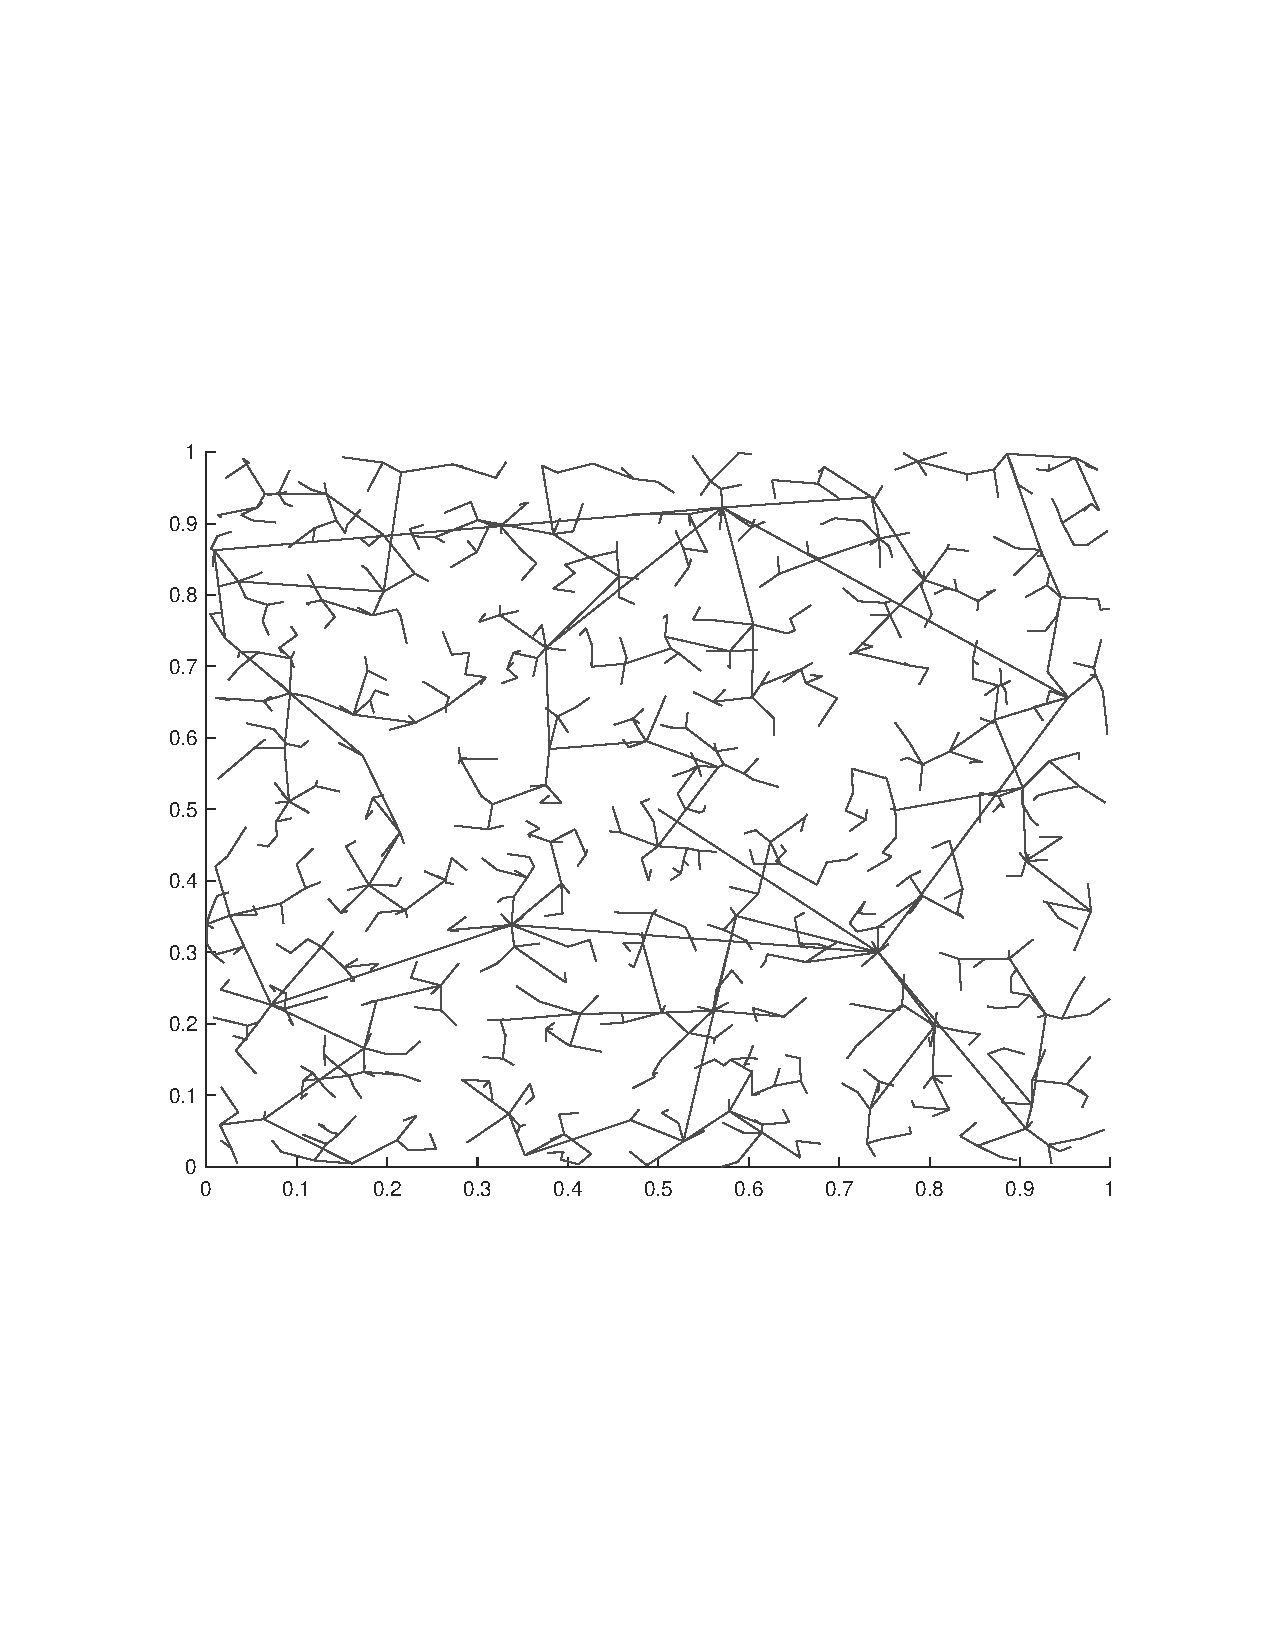
\includegraphics[width=\textwidth]{plainRRT1000}
    \caption{RRT-tree after 1000 iterations.}
  \end{subfigure}
  \begin{subfigure}[b]{0.3\textwidth}
    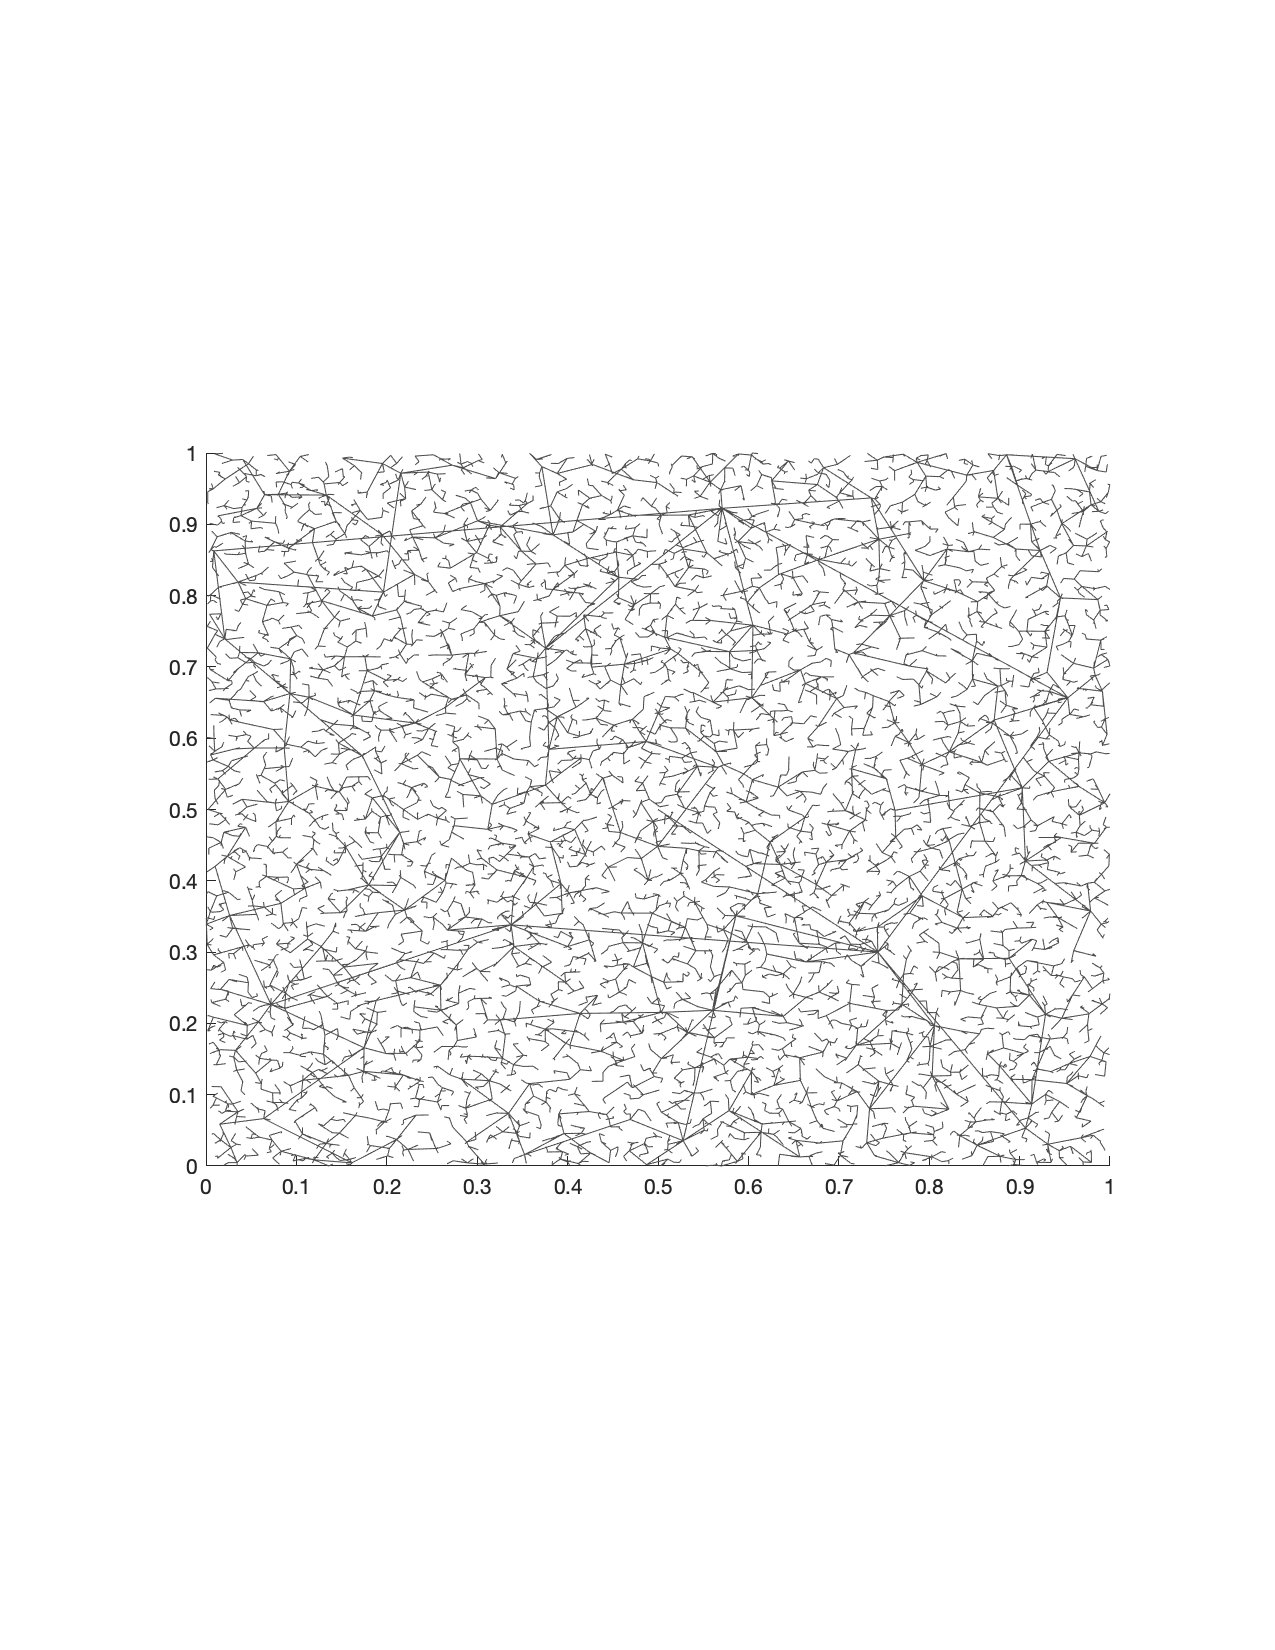
\includegraphics[width=\textwidth]{plainRRT10000}
    \caption{RRT-tree after 10000 iterations.}
  \end{subfigure}
\end{figure}

\subsection{General framework under differential constraints} (LaValle p.676.)


\subsection{RDT}


\subsection{Dynamic RRT}

\subsection{Funnel}

A Funnel is a motion primitive that is 'guaranteed' to take the vehicle from a
set of initial conditions to a set of goal states. 

\subsubsection{Composition of funnels}

In essence the 
Each funnel solves the subgoal of getting from the initial set of the funnel to
the goal set. Thus in essence each funnel solves the subproblem of getting from
one funnel to the next, and therefore composing funnels from some global initial
state to the goal state will have solve the motion planning problem with the
guarantees given by the tubes used for the planning task at hand.

TODO - insert pretty picture of funnel with the integral curves of the extremal
paths embedded in beautiful red.

\subsubsection{Reachability plot for the Ground-Vehicle}
TODO - plot the reachability for the ground-vehicle in some time interval using
simulations. 

TODO - plot A reachability tree in 3D using funnels - because different theta's
can exists at the same x,y positiions.

\subsection{Sampling}
It is important that the sampling sequence is dense in the space where sampling
occurs (state-space?), as we want resolution completeness in the end.
\subsubsection{How to obtain uniform sampling}
\subsubsection{How to define a good distance metric}
In general, it is not possible to get a perfect distance metric for our planning
problem, as this involves solving another optimal planning problem, and will
therefore be as, or more complex than the motion planning problem which is
already being solved. Therefore in general we will have to limit ourselves to
approximate distance metrics. The idea is to get as close to the optimal
cost-to-go function without having to compute expensive computations \cite{LaValle09}.
Distance metrics candidates in the RRT-Funnel algorithm:
\begin{itemize}
  \item Time - Since time can be found by simple summing up the time of all the
    funnels which need be added to get to the certain point in the configuration space.
  \item Lyapunov function - As the Lyapunov function can be seen as an energy
    function, the cost to go to a point can (probably) be used as a metric in
    the planning.
  \item Length of the shortest path between two configurations - ignoring collisions.
  \item A* search heuristics.
  \item Geometric - Stacking Funnels, where the shortest funnel of funnels wins.
    e.g. if the point is not in the cone projected out from the current state by
    the current motion primitives, pick the most extreme turn, and start over
    once again. If it can be reached by a turn, turn, then go straight for N-Funnels.
\end{itemize}

Note that most of these metrics are not metrics in the full sense, as they do
not fulfill the symmetric property, as under dynamic constraints going from a to
b, may not be the same as going from b to a. In most cases it is not true for a
nonholonomic vehicle.

\subsubsection{How to extend the tree?}

Should it be expanded into the dynamic Voronoi regions? If so, what are these regions?


\subsection{Motion Primitives}

A motion primitive is a discrete action chosen from some action set
\(\modelactionspace{}\), and applied as a constant action over a fixed period of
time. The time periods can vary in length, as the primitives do not need to have
the same time length. Thus in the model:

\begin{math}
  x_{k+1} = f_d(x_k,u_k)
\end{math} 

Where \(x_k = x((k-1)\delta{}t)\), and \(u_k\) is the action in
\(\modelactionspace{}_d\) that is applied from time \((k-1)\delta{}t\) to
\(k\delta{}t\). If we let \(\overline{u}^p\) be a motion primitive in
\(\modelactionspace{}\), which is a function from an interval of time, unto
\(modelactionspace{}\). Then by letting the interval of time start at 0 and stop
at \(t_F(\overline{u}^p)\), which has a final time that depends on the
particular prmitive \cite{LaValle09}.


\subsection{Reachability Graph}

\subsection{RRT-Funnels}


\subsubsection{Transforming and composing the tubes}

If we look at the cyclic coordinates of our model, we can see that using 'cyclic
coordinates', the dynamics is independent of position. Or rather:

\begin{math}
  \dot{\dot{q}} = \mathcal{L}(\dot{q},q)
\end{math}

TODO - finish this.


\subsubsection{Using Funnels as motion-primitives}

\subsubsection{Designing good motion primitives}

    \part{Method}
    \chapter{Method}

This chapter will introduce and develop the \rrtfunnel{} algorithm, by two
means: First develop robust motion primitives through the \ac{SOS} programming
framework based on the work in~\cite{majumdarFunnelLibrariesRealtime2017}, and
second, deploy these funnels as robust motion primitives in a discrete \ac{RRT}
robust motion planner based on~\cite{lavalleLav98cPdf}. Using \textit{robust}
motion primitives has several advantages. Firstly, they are robust to
uncertainty, and thus, as long as the uncertainties in the system are akin to
the assumptions put on the incoming uncertainty parameters, the vehicle will not
leave the funnel, and hence if the funnel is not in collision, neither will the
system be. Secondly, with the assumption that the motion primitives are robust,
there is no need for more conservative maneuvers and heuristics, such as
maximizing the distance to an obstacle. The system might as well choose a
primitive that is close to an obstacle, as one that is far away, as the funnel
is guaranteed to be collission-free in both cases. This means that a robust
motion primitive algorithm can perform more aggressive maneuvers than one that
is inherently conservative about its environment and
maneuvers~\cite{singhRobustOnlineMotion2017}.

\section{Generating robust motion primitives}

In order to create a basic set of funnels as the robust motion primitives for
the \rrtfunnel{} motion planning algorithm, a few obstacles has to be overcome.
The first one is settling on a dynamical system model for the funnel
calculations. This thesis employs the simple unicycle model from
\cite[LaValle.p~613]{Lav06} which is modified slightly into
\begin{equation}
  \label{eq:model-dynamics}
  \mathbf{x} =
  \begin{bmatrix}
    x \\ y \\ \theta \\ \dot{\theta} \\
  \end{bmatrix}, \, \dot{\mathbf{x}} =
  \begin{bmatrix}
    -v(t)\sin(\theta) \\
    v(t)\cos(\theta) \\
    \dot{\theta} \\
    u \\
  \end{bmatrix},
\end{equation}
which is a second-order unicycle model with constant speed. A picture of the
model can be found in figure~\ref{fig:second-order-unicycle}.
\begin{figure}
  \centering
  {
    \fontsize{16pt}{16pt}\selectfont
    \def\svgwidth{1.333in}
    \import{figures/method/}{unicycle-model.pdf_tex}
  }
  \caption{The unicycle model of a vehicle.}
  \label{fig:second-order-unicycle}
\end{figure}
Although this is the only model used in this thesis, the framework and the code
is easily adapted into accommodating a different and more complicated model.

\subsubsection{Generating the trajectories}

The robust motion primitives are \textit{finite regions of time variance} around
an initial trajectory, meaning that they are verified regions of the state space
surrounding a trajectory in which the system can reach in a given time interval,
also called a reachable set~\ref{subsec:reachable-set}. But in order to verify
the robust regions surrounding a trajector, first the trajectories themselves
have to be generated. Generating optimal trajectories is a rich field in the
motion planning literature~\cite{bettsSurveyNumericalMethods}, and the initial
trajectories could have been generated through any number of methods, however,
the \textit{direct collocation method} was chosen as it builds locally optimal
trajectories from a discrete set of sampled points along a sought trajectory,
which is beneficial for the discrete funnel verification
in~\ref{subsec:generating-funnels}.

Since it is an optimal trajectory planner, a cost function has to be chosen for
the solver to minimize, which in this case is:
\begin{equation}
  J = \int_{0}^{T} \left[ 1 + {u_{0}}^{T}Ru_{0} \right] dt
\end{equation}
from~\cite{majumdarRobustOnlineMotion2013}.

An example of an initial trajectory set is pictured
in~\ref{fig:initial-trajectories}, and consists of a left-turn, a
straight-forward, and a right-turn motion primitive.

\begin{figure}
  \centering
  \begin{minipage}[b]{0.2\textwidth}
    
\includegraphics[width=\textwidth]{figures/method/straight-trajector}
  \end{minipage}
  \hfill
  \begin{minipage}[b]{0.2\textwidth}
    
\includegraphics[width=\textwidth]{figures/method/left-trajector}
  \end{minipage}
  \hfill
  \begin{minipage}[b]{0.2\textwidth}
    
\includegraphics[width=\textwidth]{figures/method/right-trajector}
  \end{minipage}
  \caption{Three motion primitives for the \rrtfunnel{} algorithm, one
    straight, one left, and one right turn.}
  \label{fig:initial-trajectories}
\end{figure}

\subsubsection{Initializing the funnel calculations with a TVLQR candidate as
  the initial Lyapunov function}

The funnel calculation algorithm has to be initialized with a candidate Lyapunov
function. In the same way
as~\cite[Majumdar]{majumdarFunnelLibrariesRealtime2017}, the funnel generation
algorithm will be initialized with a \ac{LQR} controller as the initial Lyapunov
function employing a cost function of the form
\begin{equation}
  J = x^{T}(t_1)F(t_1)x(t_1) + \int_{t_{0}}^{t_{1}} \left( x^{T}Qx + u^{T}Ru + 2x^TNu \right) \mathrm{dt},
\end{equation}
which when employed on the linearization of the system dynamics
\begin{equation}
  \dot{\bar{x}} \approx A(t)\bar{x}(t) + B(t)\bar{u}(t) +D(t)w(t),
\end{equation}
gives an initial candidate Lyapunov function
\begin{equation}
  V(t,x) = {\bar{x}}^{T}S_{i}\bar{x}.
\end{equation}
where \(S_{i}\) is a solution from the \textit{Ricatti} equation associated with
the \ac{LQR} controller.

\subsubsection{Generating the funnels around the trajectories}
\label{subsec:generating-funnels}

With the nominal trajectories, and the initial Lyapunov functions ready, the
funnels around the nominal trajectories can be calculated using the
algorithm~\ref{alg:funnelalgorithm}, and is implemented in software through the
~\cite[sostools]{sostools} toolbox.

However, two obstacles remain, as the dynamics for the
model~\eqref{eq:model-dynamics} are still not polynomial, and the \ac{SOS}
method can only verify polynomial systems. Thus in order to obtain the needed
polynomial dynamics, the system is expanded around the nominal trajectory with a
Taylor expansion of degree three. Secondly the function limiting the size of the
funnel \(\rho(t_{k})\) has to be initialized by a feasible \(\rho(t)\). This is
done through the equation
\begin{equation}
  \rho(t_{k}) = \mathrm{exp}\left( \rho_{\tau}\frac{\left( t_{f} - t \right)}{\left( t_{f} - t_{0}  \right)}\right) + \rho_0
\end{equation}
from~\cite[eq.~6.sec~3]{tobenkinInvariantFunnelsTrajectories2010}, where
\(\rho_{\tau}\) is a positive constant determining the upper bound on the
funnel, along with the zero value \(\rho_0\). If the given choice of
\(\rho_{\tau}\) does not verify a funnel, either increase the value of
\(\rho_{\tau}\) and \(\rho_0\), and optionally the number of sampled points from
the trajectory to be verified~\cite{tobenkinInvariantFunnelsTrajectories2010}.

Thirdly, the initial condition set has to be decided beforehand. In general the
initial condition set can be any semi-algebraic set in the state-space. However,
a simple way of obtaining an initial condition set for the trajectories at hand
is by taking advantage of the Lyapunov function canditate from the
\ac{LQR}-controller. Thus by setting
\begin{equation}
  \mathcal{X}_{0} = \frac{S_{k}}{\rho_{\tau}}
\end{equation}
an intial condition is obtained. However, any semi-algebraic set will do, and
the algorithm is not constrained to this one initial condition set in
particular, but it has proven itself useful when calculating new motion
primitives for a system when the initial condition set is not obvious. Another
idea is to use the outlet of one funnel as the initial condition set for the
calculation of another.

For the cost function in the funnel generation
algorithm~\ref{alg:funnelalgorithm}, which in general is a maximization of the
determinant of the upper bound ellipse for the funnel set, one may not be
concerned about the size of the hyperellipsoid in all directions of the
state-space. As an example: For the vehicle model in this thesis the size of the
funnel projected down into the xy-plane will be the most important metric.
Whether or not the vehicle's orientation parameter \(\theta\) is close to the
nominal heading is of less concern, and is therefore down-prioritized, along
with the cost on the control input \(u\). Having a large \(\theta\) and
\(\dot{\theta}=u\) semi-axis in the hyperellipsoid can also be beneficial, as it
increases the inlet of the ellipsoid at hand. 

The funnels in this thesis are parametrized as sub-level sets of a Lypunov
function for which the state-space does not invalidate the sub-level constraint.
A visualization of the Lyapunov function associated with a straight motion
primitive can be found in~\ref{fig:visualized-lyapunov}.
\begin{figure}
  \centering
  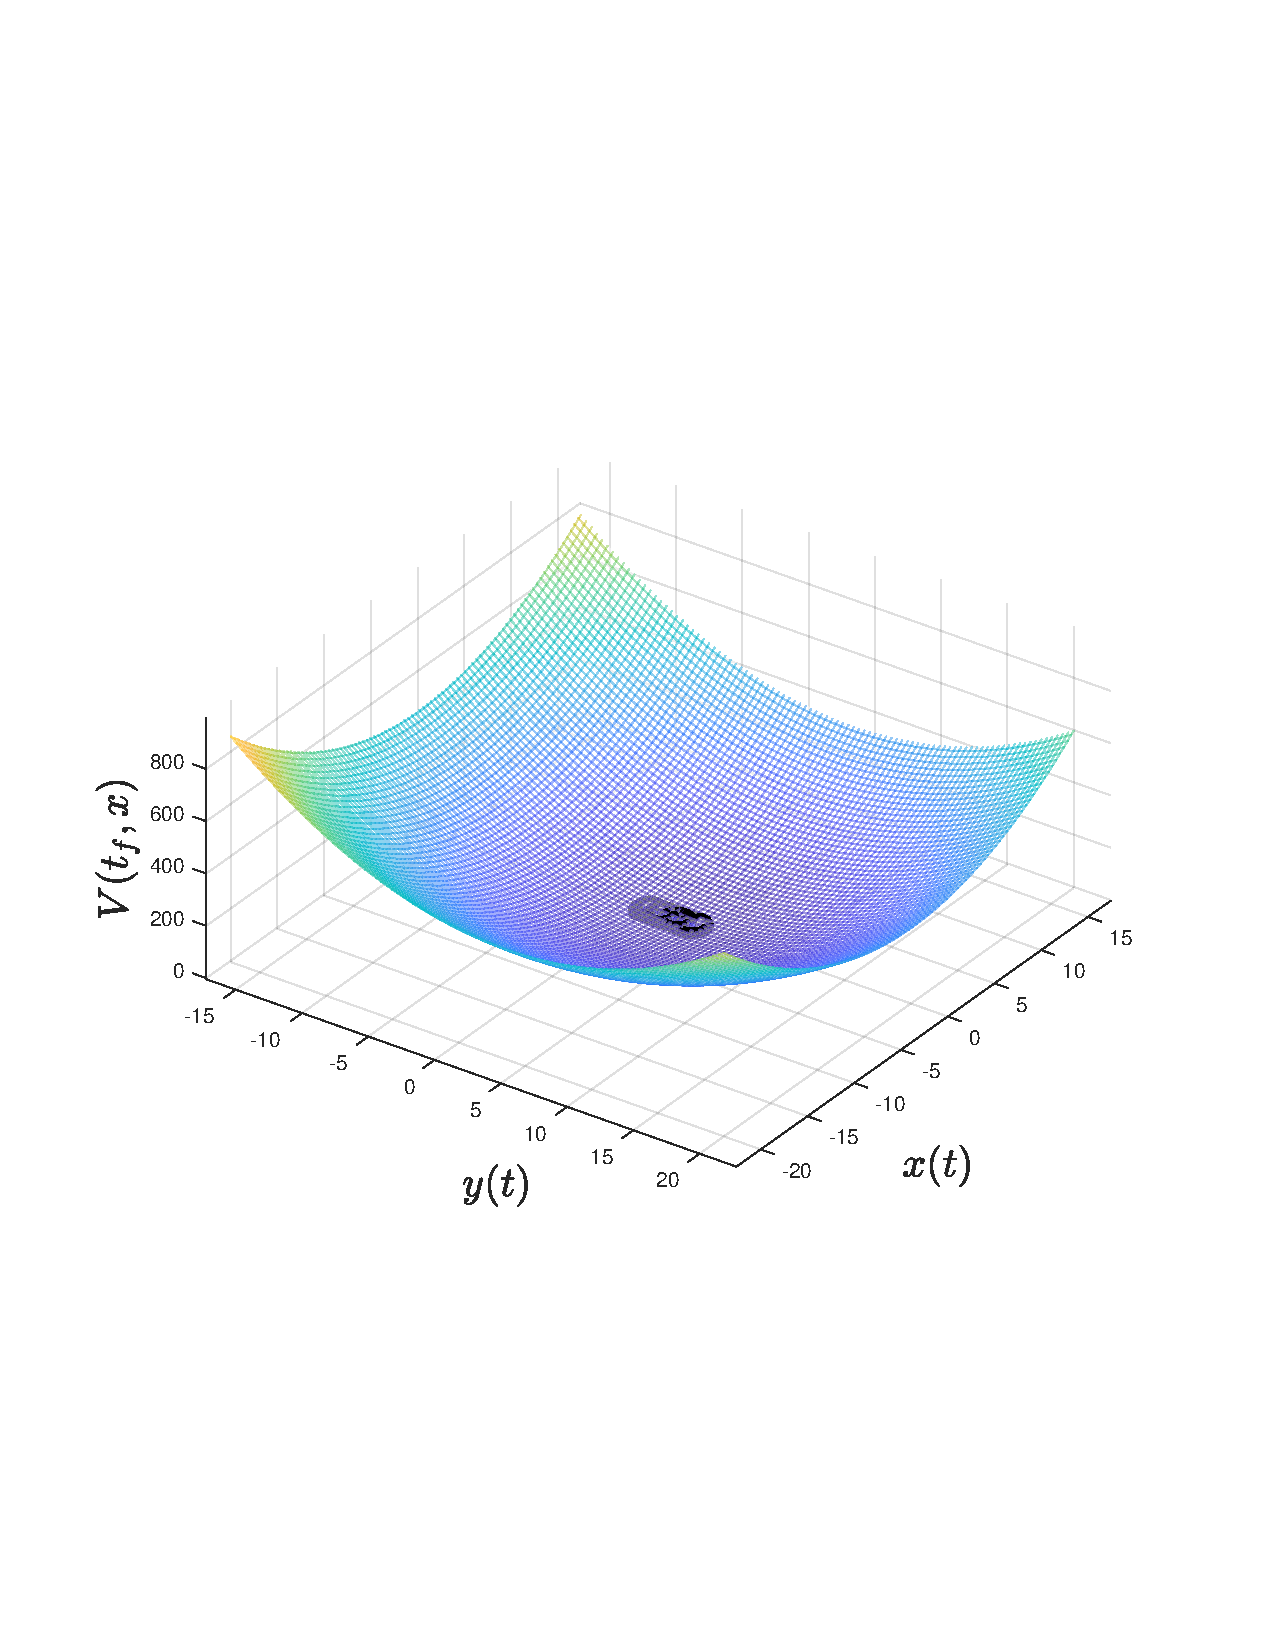
\includegraphics[scale=.3]{figures/rrtfunnel/straight-funnel-lyapunov-3d}
  \caption{A visualization of the Lyapunov function values around a straight
    motion primitive.}
  \label{fig:visualized-lyapunov}
\end{figure}

\subsection{Only minimizing the volume of the funnel projected down into the
  xy-plane}
\label{subsec:xy-cost-function}

For the \rrtfunnel{} algorithm, the size of the of the hyperellipsoid which
contains the reachable set is not equally important in all dimensions, as
mentioned in~\ref{subsec:generating-funnels}. In the forest traversal case the
size of the elipsoid in the \(\theta\) and \(u\) dimensions are unimportant.
There is no need in minimizing the value of \(\dot{\theta}\), as they will not
make the traversal of the forest any easier, in fact they might inflate the size
of the \((x,y)\) ellipsoid.

Therefore in order to minimize the actual size of the funnel where the physical
vehicle can move in the world space modify the costfunction according to
\cite{majumdarFunnelLibrariesRealtime2017}. Thus, given a projection map \(\pi :
\R^n \rightarrow \R^{n_p}\), and the ellipsoid \(\mathcal{E} = \set{\bar{x} \in
  \R^n | \bar{x}^TS_{k}\bar{x} \leq 1}\) with
\[
  S_k^{(p)} = \p{PS_k^{-1}P^T}^{-1}
\]
where \(P\) is an \(n\times n_p\) projection matrix.

Since minimizing the volume of the ellipsoid \(\pi(\mathcal{E})\) using an \ac{SDP}
relies on maximizing the determinant of \(S_k\), and \(det(S_k)\) is a nonlinear
function of \(S_k\), the function has to be linearized in order for it to be
handled by the \ac{SOS}
framework. \cite[Majumdar]{majumdarFunnelLibrariesRealtime2017} solves this by
linearizing \(det(S_k)\) at the solution of \(S_k\) from the previous iteration,
and maximizes this linearization instead. In the end this translates to
\[
  \mathnormal{lin}\p{det\p{S_k}} =
  Tr\p{P^T\p{PS_{k,0}^{-1}P^T}^{-1}PS_{k,0}^{-1}S_kS_{k,0}^{-1}}
\]
where \(S_{k,0}\) is the nominal value for the linarization, and \(Tr\) is the
trace of the matrix.

\subsection{Searching for a controller which minimizes the size of the funnel}

With the non-optimal feedback controller given to the funnel calculation
framework (non-optimal with regards to the funnel calculation cost function),
the size of the funnels will in general be larger than if given a better
controller. Thus in order to further minmize the size of the funnel in the
xy-plane this method, along with the cost function
from~\ref{subsec:xy-cost-function} is used to make traversal through obstacles
in the world space easier. Hence, referring to~\cite[Majumdar.sec~4.3.2
(Feedback control synthesis)]{majumdarFunnelLibrariesRealtime2017}, the initial
controller input to the algorithm can be optimized with the goal of minimizing
the size of the funnel, given a few conditions on the system.

Firstly the system needs to be control affine:
\begin{equation}
  \dot{x} = f(x(t)) + g(x(t))u(t)
\end{equation}
so that the control policy can be parametrized as a polynomial
\(\bar{u}_f(t,\bar{x})\), and the system dynamics written as:
\begin{equation}
  \dot{\bar{x}} = f(x_0(t) + \bar{x}(t)) + g(x(t))\left[ u_0(t) + \bar{u}_f(t,\bar{x}) \right] - \bar{x}_0
\end{equation}
Then the feedback controller can be optimized by adding the coefficients of the
polynomial \(u_f(t,\bar{x})\) to the set of decision variables in the original
optimization problem. The only issue is that now \(\dot{V}\) is bilinear in the
decision variables \(V\) and \(\bar{u}_f\)
\begin{equation}
  {
    \newcommand{\Vdot}{\dot{V}}
  \Vdot(t,\x) = \frac{\partial V(t,\x)}{\partial \x} \dot{\x} + \frac{\partial V(t,\x)}{\partial t}
  }
\end{equation}
Thus in order to minimize the cost function a search is done in
\((\bar{u}_f,\rho,L_t,L_{0,i},S_k)\) while keeping \((V,L,L_{\epsilon,k})\)
fixed. This method combined with the uncertainty added
in~\ref{sec:adding-uncertainty}, is what forms the basis of the funnel
computations as robust motion primitives for traversal in a dense forest
environment, as summarized in algorithm~\ref{alg:funnelalgorithm-extended}.

\begin{algorithm}[H]
  \caption{Feedback Funnel computation}
  \label{alg:funnelalgorithm-extended}
  \DontPrintSemicolon \SetAlgoNoLine

  \KwIn{\(V\) and \(\rho\)} \KwOut{Funnel}

  \(cost_{prev} = \infty\)\; converged = false \; \While{\(\neq converged\)}{
    Optimization problem 1: \;
    \begin{align*}
      \underset{\substack{\bar{u}_f,L,L_{t},L_{0,i},S_{k},L_{}}}{\inf}&  \sum_{k=1}^{N} \vol(\mathcal{E}(t_{k}))& \\    
      \text{subject to } & V \text{ and } \rho \text{ constant.}& \\
    \end{align*}\;
    Optimization problem 2: \;
    \begin{align*}
      \underset{\substack{\bar{u}}_f,\rho,L_{t},L_{0,i},S_{k}}{\inf}&  \sum_{k=1}^{N} \vol(\mathcal{E}(t_{k}))& \\    
      \text{subject to } & (V,L,L_{\mathcal{E},k}) \text{ constant.}& \\
    \end{align*}\;
    Optimization problem 3: \;
    \begin{align*}
      \underset{\substack{V,\rho, L_{t},L_{0,i},S_{k}}}{\inf}&  \sum_{k=1}^{N} \vol(\mathcal{E}(t_{k}))& \\    
      \text{subject to } & (L,L_{\mathcal{E},k},\bar{u}_f) \text{ constant.}& \\
    \end{align*}\;
    cost = \(\sum_{k=1}^{N} \vol(\mathcal{E}(t_{k}))\) \;
    \If{\(\frac{cost_{prev} - cost}{cost_{prev}} < \epsilon\)} {
      converged = true
    }\;
    \(cost_{prev} = cost\)\;
  }\;
\end{algorithm}


\subsection{Adding uncertainty to the funnel calculation}
\label{sec:adding-uncertainty}

The system dynamics and funnel generation theory presented this far has not been
able to handle any system uncertainty, which is vital to the safe execution of
the \rrtfunnel{} algorithm. However, the basic formulations presented do have
all the necessary formulations present, and adding uncertainty is equivalent to
adding another constraint to the optimization
problem~\eqref{opt:sufficient-conditions}.

Following are the changes to the formulation of the \ac{SOS} optimization
condition~\eqref{eq:funnelsufficient}
from~\cite{majumdarFunnelLibrariesRealtime2017} so that a funnel takes into
account a bounded uncertainty term of the form \(\mathcal{W} = \set{ w(t) \in
  R^d \mid g_{w,j}(w) \geq 0\, \forall j = 1,\ldots,N_w}\). But first the
uncertainty has to be added to the system dynamics equation. This is done
through adding an uncertainty term \(w\)
\begin{equation}
  \dot{\bar{x}} = f_{cl}(t, \bar{x}(t), w(t)).
\end{equation}
Then the requirement~\eqref{eq:reachableset} is slightly modified so that
\begin{equation}
  \label{eq:uncertain-reachableset}
  \bar{x}(0) \in \mathcal{X} \implies \bar{x}(t) \in F(t),\, \forall t \in
  [0,T], \, \forall w \colon [0,T] \rightarrow \mathcal{W}
\end{equation} 
where \(F(t)\) is the new reachable set for the uncertain system. Thus the
sufficient condition~\eqref{eq:funnelsufficient} turns into
\begin{equation}
  \label{eq:funneluncertain-sufficient}
  V(t,\bar{x}) = \rho(t) \implies \dot{V}(t,\bar{x},w) < \dot{\rho}(t), \, \forall t \in [0,T], \, \forall w(t) \in \mathcal{W}.
\end{equation}
The Lyapunov function derivative then becomes
\begin{equation}
  \dot{V}(t,\bar{x}, w) = \frac{\partial V(t,\bar{x})}{\partial x} f_{cl}(t,\bar{x},w) + \frac{\partial V(t,\bar{x})}{\partial t},
\end{equation}
and the optimization condition~\eqref{eq:optimizationconditionsos} turns into
\begin{align}
  \label{eq:optimizationconditionuncertain}
  \dot{\rho}(t) - \dot{V}(t,\bar{x},w) - L(t,\bar{x},w) \left[ V(t,\bar{x}) - \rho(t) \right] - L_{t}(t,\bar{x},w)\left[ t\left( T - t \right) \right]  & \nonumber \\
  - \sum_{j=1}^{N_{w}} L_{w,j}(t,\bar{x},w)g_{w,j}(w) \quad \text{is SOS} &  \\
  L_{w,j}(t,\bar{x},w) \qquad \text{is SOS}, \; \forall j = 1,\ldots,N_w \nonumber
\end{align}

\subsubsection{Shifting funnels and invariance}

Now that the funnels are able to be calculated for a basic set of motion
primitives, it is time to start looking at chaining motion primtives together in
order to construct longer and more complex motion primitives from a set of basic
motions. Thus, in order to freely shift funnels around in the configuration
space, the cyclic coordinates of the system has to be determined, so that the
dynamics of the system is never violated, even though the funnels now start and
end in a completely different part of the configuration space, the original
dynamics must not be violated. Therefore the cyclic and non-cyclic coordinates
of the system must be decided~\ref{subsec:cyclic-coordinates}. Therefore, given
the model~\ref{eq:model-dynamics} the cyclic coordinates of the system are:
\begin{align}
  \mathcal{L} &= T - V = \frac{1}{2} mv^2 + \frac{1}{2}I\dot{\theta}^2 \\ 
              &= \frac{1}{2} 
                m\begin{bmatrix}
                  -v\sin \theta \\ 
                  v \cos \theta \\
                \end{bmatrix}^{T}
  \begin{bmatrix}
    -v\sin \theta \\
    v \cos \theta \\
  \end{bmatrix}
  + I\dot{\theta}^2 \\
              &= m \left(
                v^2 \sin^2 \theta + v^2 \cos^2 \theta
                \right)  + I {\dot{\theta}}^2 \\
              &= mv^2 + I {\dot{\theta}}^2 \\
\end{align}
which shows that the LaGrangian is invariant to shifts in the \((x,y,\theta)\)
variables, since \(\frac{\partial\mathcal{L}}{\partial q_i} = 0 \, q_i =
x,y,\theta\). Hence now, any funnel in the base set can be shifted freely around
in the cyclic coordinates of the system withouth changing the solution to the
system dynamic equation, and thus create an infinite set of funnels in the state
space for the planner to work with. Through the partitioning of coordinates into
cyclic- and non-cyclic coordinates of the form \(x = [x_c x_{nc}]\), the state
dynamics \(\dot{x} = f(x(t), u(t))\) only depends on the non-cyclic coordinates
of the system. Thus, a trajector of the form \(t \rightarrow (x(t),u(t))\) which
solves \(\dot{x} = f(x(t),u(t))\) can then be transformed through a shift
\(\Psi_c\) along the cyclic coordinates of the system to yield a valid solution
of the form
\[
  t \rightarrow (\Psi_{x}(x(t)), u(t))
\]
where the transform \(\Psi\) is given by
\[
  \Psi([x_c, x_{nc}]) =  
  \begin{cases}
    x_c \rightarrow \hat{x}_{c} \\
    x_{nc} \rightarrow x_{nc} \\
  \end{cases}.
\]

\subsection{Sequential funnel composition}
\label{sec:composable-funnels}

Now that funnels can be shifted freely around the configuration space along the
cyclic coordinates of the system to create new motion primitives it is time to
start chaining funnels together to create trees of funnels that span out into
the planning environment in orderr to create a robust motion plan. However, in
order for two funnels to create a third and new motion primitive when chained
together they need to be composable, which means that the inlet of the second
funnel needs to be fully contained within the outlet of the first one. Otherwise
the robustness guarantees of the traversal will be lost. An abstract pictorial
representaion of two funnels composed together can be seen
in~\ref{fig:two-funnels-composed} to emphasize this observation. The
mathematical definition of funnel composition~\ref{def:funnel-composition}
that is used to verify that two funnels are composable, and is implemented as a
\ac{SOS}-program in~\ref{AppendixB}. However, take note that the definition
has to be modified slightly in order to take into account the translation along
the cyclic coordinates. Hence the definition used
is~\cite[definition~3,sec~5]{majumdarFunnelLibrariesRealtime2017} which states
\begin{definition}
  An ordered pair \(F_1,F_2\) of funnels \(F_1 \colon [0,T_1] \rightarrow
  \mathcal{P}(\R^n)\) and \(F_2 \colon [0,T_2] \rightarrow \mathcal{P}(\R^n)\)
  is \textit{sequentially composable modulo invariances} if there exists a shift
  along cyclic coordinates such that \(F_{1}(T_1) \subset
  \Psi_{c}\left(F_2(0)\right)\)
\end{definition}
In laymans terms this means that if a funnel \(F_2\) can be shifted along cyclic
coordinates to stack up against the outlet of funnel \(F_2\) so that they are
composable in the sense of definition~\ref{def:funnel-composition}, they are
composable modulo invariances. Hence, any funnel in the configuration space will
be a set consisting of the funnel from the basic set, along with a
transformation along the cyclic coordinates of the system \(\hat{\mathcal{F}} =
\set{F_n \in \R^n \mid \Psi_{c,i}(F_i), F_i \in \mathcal{F}}\), where
\(\mathcal{F}\) is the basic set of funnels.

\begin{figure}
  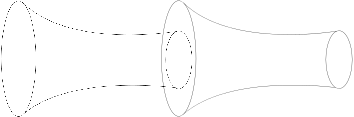
\includegraphics[scale=.2]{figures/method/funnel-composition} \centering
  \caption{Two funnels that can be successfully composed, as the outlet of the
    first one is fully contained in the inlet of the second.}
  \label{fig:two-funnels-composed}
\end{figure}

Using the generalized S-procedure
\begin{equation}
  V_1(T_1,\bar{x}) \leq \rho_1(T_1) \implies V_2(0, \bar{x}) \leq \rho_2(0)
\end{equation}
the composability of two funnels can be checked through the \ac{SOS} program
\begin{align}
    & \text{Find } && L(\bar{x}) \\
    & \text{s.t. } && \rho_2(0) - V_2(0,\bar{x}) - L(\bar{x})\left( \rho_1(T_1) - V_1(T_1,\bar{x}) \right) \text{ is SOS} \nonumber \\ 
    &&& L(\bar{x}) \text{ is SOS} \nonumber
\end{align}

\subsection{Checking the conservativeness of the funnel calculated}

The funnels generated are \textit{Outer approximations} of time reachable sets
for the system at hand. This means that in general they are larger than the
actual reachable set for the system. This can be verified through a Monte-Carlo
simulation for the straight funnel primitive. Therefore, running N-simulations
from the funnel inlet, and storing the solutions, it is possible to visualize
the actual funnel for the system, and one such can be seen
in~\ref{fig:funnel-simulated-overlaid}.

By comparing one of the funnels in the funnel set with a funnel based from
\(10.000\) simulation runs, it is seen that the calculated funnels are indeed
proper outer approximations of the time-reachable sets for the dynamical system.
Therefore, the conclusion is that the uncertain trajectories are contained
within the funnels used in the planner, and the trajectories can be seen as
robustly to uncertainty given the uncertainty and dynamical assumptions made.

\begin{figure}
    \begin{subfigure}[b]{0.3\textwidth}
        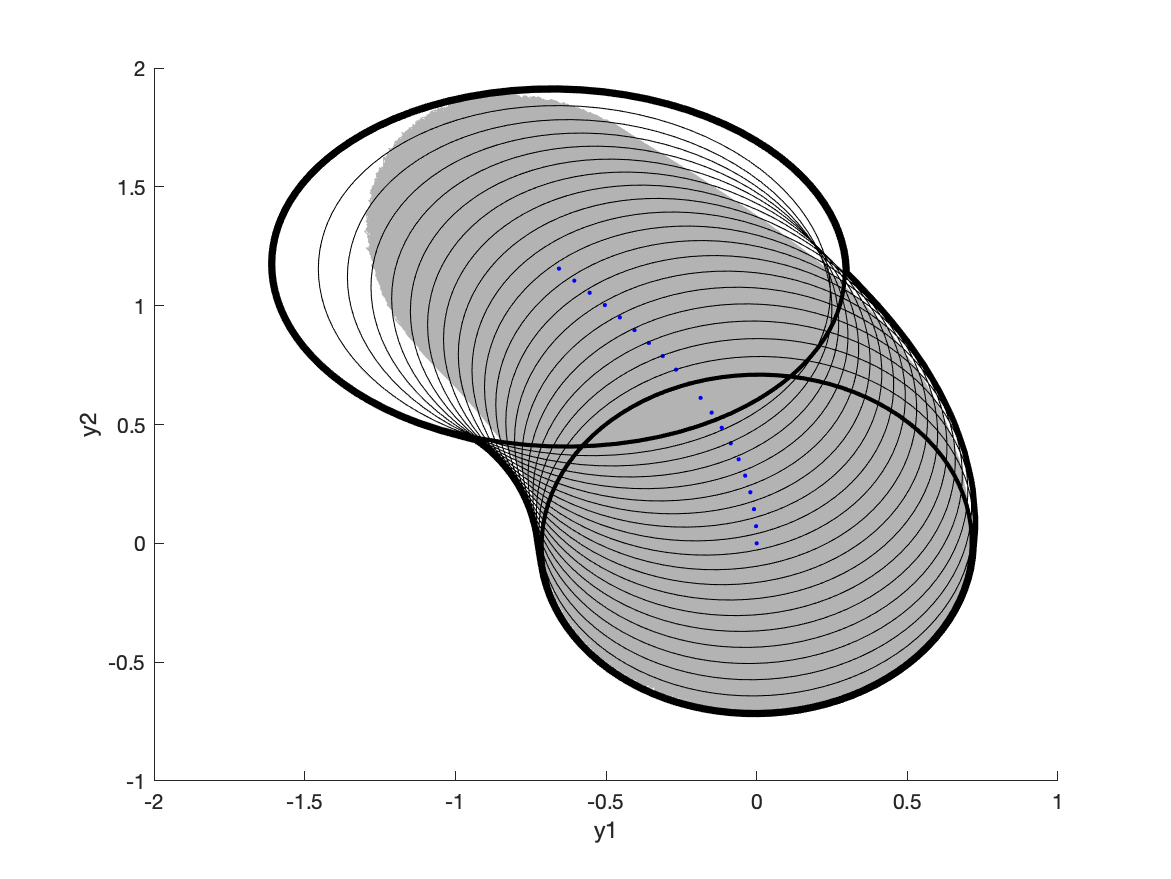
\includegraphics[width=\textwidth]{figures/experiments/FunnelSim4}
    \end{subfigure}
     %add desired spacing between images, e. g. ~, \quad, \qquad, \hfill etc. 
      %(or a blank line to force the subfigure onto a new line)
    \begin{subfigure}[b]{0.3\textwidth}
        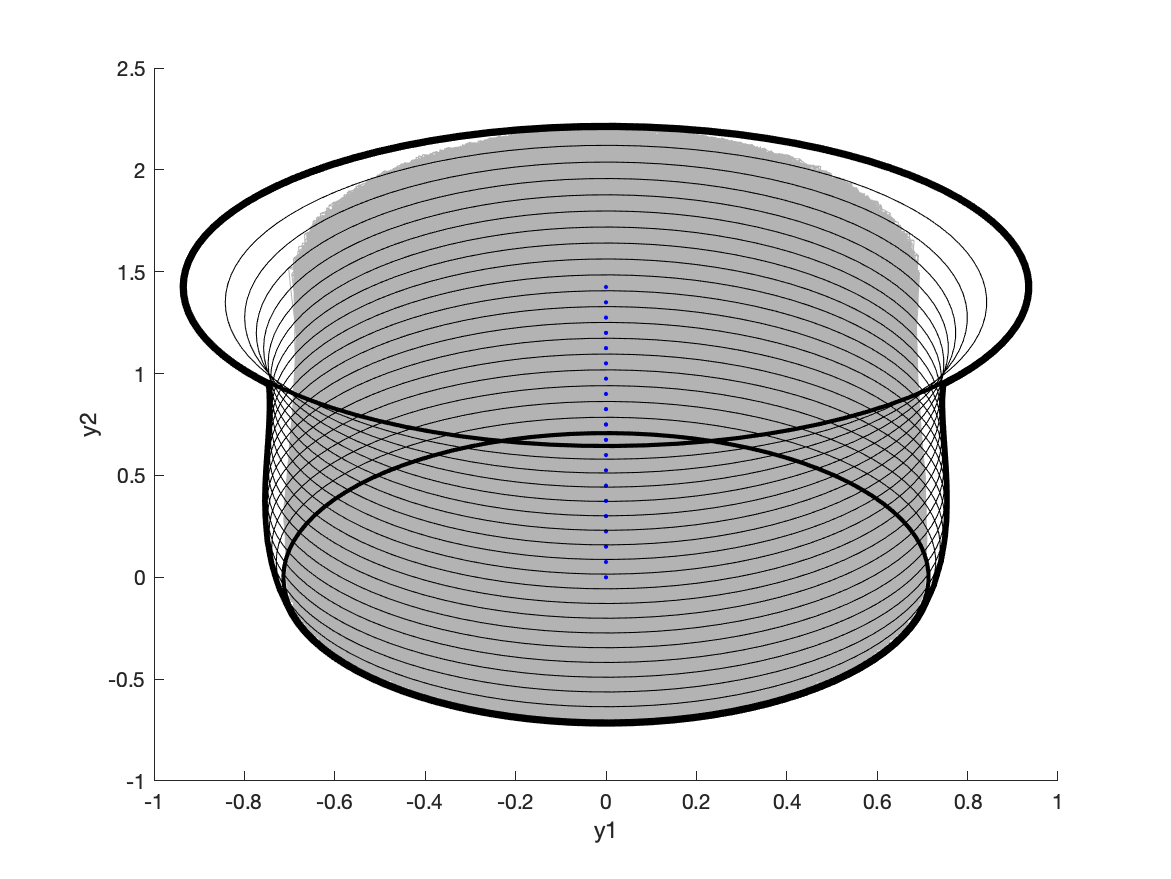
\includegraphics[width=\textwidth]{figures/experiments/FunnelSim1}
    \end{subfigure}
    \begin{subfigure}[b]{0.3\textwidth}
        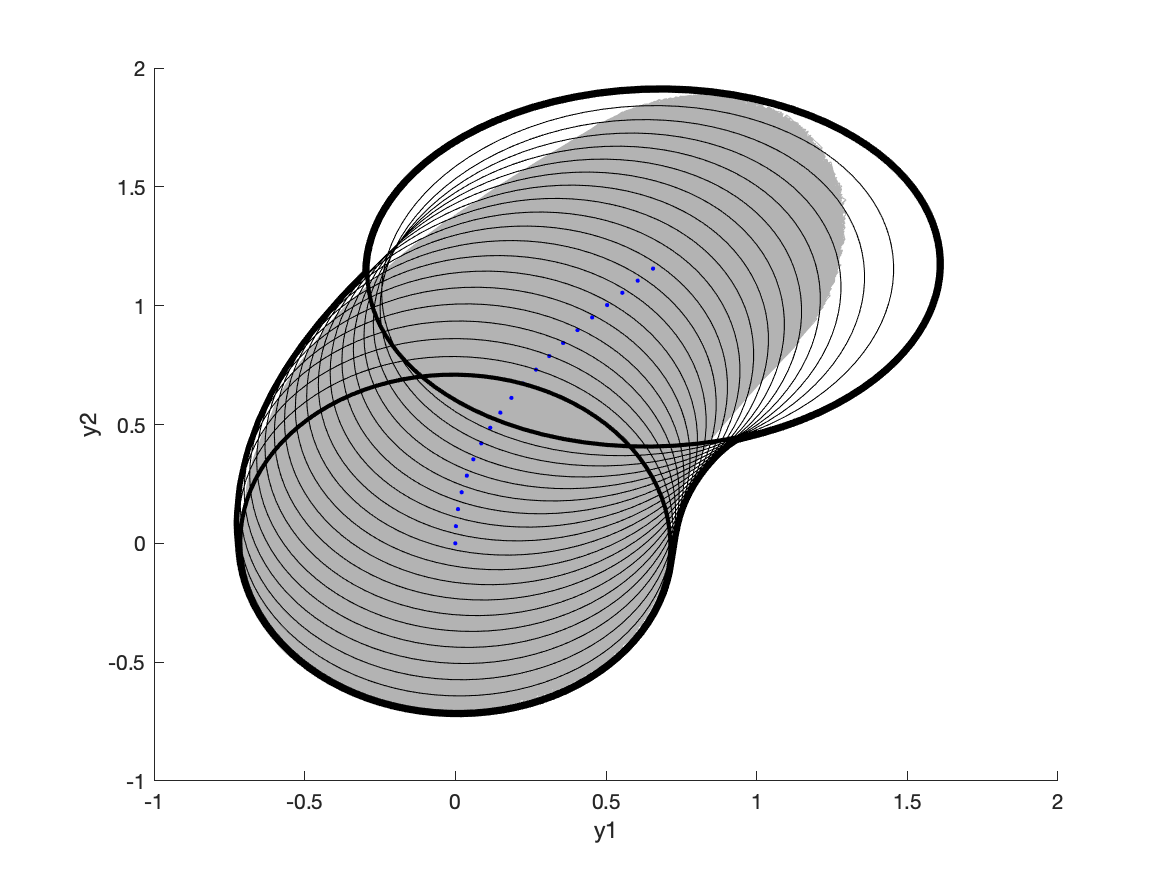
\includegraphics[width=\textwidth]{figures/experiments/FunnelSim5}
    \end{subfigure}
     %add desired spacing between images, e. g. ~, \quad, \qquad, \hfill etc. 
      %(or a blank line to force the subfigure onto a new line)
    \caption{The simulated trajectories, overlaid with the outer approximation
      that is the funnel returned by the \ac{SOS} calculation for three
      trajectories from the trajectory library \(\mathcal{T}\).}
    \label{fig:funnel-simulated-overlaid}
\end{figure}

\subsection{The initial condition set for each funnel}

In order to stack funnels one after the other it is necessary for the funnels to
have a big inlet, and a smaller outlet as defined in hyperspace. It is from the
formulations in (ref perliminaries) to constrain the intial condition set for
each funnel. This is done with

The intial theta is limited to: (Make pretty figure with the intial conditions
for theta at each point (x,y))

\section{RRT}

With the basic framework for dealing with funnels as motion primitives
constructed, it is time to build the \ac{RRT} part of the \rrtfunnel{}
algorithm. The reason for choosing to base the global path planning framework on
the \ac{RRT} motion planning algorithm are as follows. One, it has the ability
ot quickly expand deep into the search-space, and then later progress towards a
finer sampling, which is valuable as it avoids local minima. Two, the \ac{RRT}
algorithm is easily extendable to larger state space, and thus adding to the
generality of the \rrtfunnel{} algorithm, such that it can be adapted to fit a
wide range of dynamical systems, as well that it has only three main components
that needs to be in place in order for successful path planning to happen in an
arbitrary configuration space. This is beneficial as most all of the complexity
accompanied with the planning problem (like uncertainty and controller
calculations) has already been handled by the \ac{SOS} framework, and hence the
\ac{RRT} algorithm need only concern itself with stacking one robust motion
primitive after the other without any concern for the complexities mentioned
above.

\subsection{Uniform sampling in SE(2)}

As mentioned in section~\ref{sec:rrt-sampling}, the \ac{RRT} algorithm needs
uniform sampling of the state space in order for it to function optimally, as
over- or under-sampling certain parts of the state space can lead to poor
performance. Therefore one needs to be careful when sampling from a
configuration space with non Euclidean
topology~\cite{kuffnerEffectiveSamplingDistance2004}.

If sampling from a configuration space which are formed stricly from cartesian
products of the form \(X = X_1\times X_2\times \cdots \times X_n\), and each cartesian
space is sampled uniformly, then the product will also be uniformly sampled. One
needs to be more careful when dealing with rotations however, as the probability
density measure can become non-uniform~\cite{Lav06}. Take the polar coordinates
as an example. Sampling uniformly from \(r\) and \(\theta\) does not form a
uniform sample product, as the \(pdf\) function will have a higher probability
density near the origin, as the outer circles will contain a bigger area. For
the model of a simple unicycle which moves in \(x,y,\theta\) the samples can be
generated from From~\cite{kuffnerEffectiveSamplingDistance2004} the samples can
be generated uniformly on the topological cylinder through
\[
  (x,y,\theta) = (\mathnormal{X}_{dim}rand, \mathnormal{Y}_{dim}rand, \mathnormal{\Theta}_{dim}rand)
\]
where \(rand\) is a random variable in the interval \([0,1)\), since for
\(SO(2)\), the rotations parametrized on \([0,1]\setminus\sim\) (where
\(\setminus\sim\) means that 0 and 1 are identified) can be multiplied by a
fixed constant, such as for \(2\pi\) which means that sampling will be uniform
in the configuration space of the robot from a simple cartesian product of
uniform random variables~\cite{Lav06}.

\subsection{Distance in configuration space}

Introducing a function which Measures distance between two points in
configuration space introduces a metric space on the underlying configuration
space \((\modelconfigurationspace{},\rho)\), where \(\rho\) is a distance
function. Finding a good distance function for the metric space at hand is a
hard problem. In general the ideal metric would have been the actual
\textit{cost-to-go} function for the system at hand. However calculating the
actual cost-to-go is equivalent to solving the original motion planning problem,
and is hence not viable~\cite{pengchengReducingMetricSensitivity2001}.

So, in order for the \rrtfunnel{} algorithm to efficiently explore the state
space it must have a good measure of distance between different poses in space,
without actually solving the planning problem anew. For a problem in the
Cartesian plane it is common to use the Euclidean distance, however, this is not
a good distance metric for non-holonomic vehicles, as it does not incorporate
the possible constraints of the system function, and has little bearing on the
actual cost-to-go of the system~\cite{parkFeedbackMotionPlanning2015}. In fact,
for sampling based planners such as the \ac{RRT}, the configuration space is
only sufficiently explored in the case where the distance function reflects the
true cost-to-go function~\cite{pengchengReducingMetricSensitivity2001}. Hence,
all other metrics will be a compromise of complexity and time vs efficiency.

Normally the \ac{RRT} algorithm splits the extension part into two sections. One
for identifying the closest node in the tree, and second one for the closest
extension that can be added onto the tree itself. Here a different distance
metric can be employed in each step. To reflect on the difficulty of creating a
general distance metric function have a look at the unicycle model
from~\eqref{eq:model-dynamics}. From inspection it is seen that the model is not
able to instantaneously move in a direction orthogonal to the direction of
travel, as is seen in~\ref{fig:non-holonomic-vehicle-euclidean-weakness}. Here
the distance between two points might be small in the sense of a regular
Euclidean distance metric, but due to the differential constraints on the system
model, the vehicle actually has to move far in order to reach the sought
configuration.

The \rrtfunnel{} algorithm will use the same metric for both the closest node
and in the extend operation on the funnel graph. The metric chosen is a modified
Euclidean metric which weights the angle \((\theta)\) depending on how close the
vehicle is to the final configuration and is defined as
\[
  \rho(x_{1},x_{2}) = w_{1}\norm{\mathnormal{X_{1}} - \mathnormal{X_{2}}} +
  w_{2}f(\theta_1,\theta_2)
\]
and taken from~\cite{kuffnerEffectiveSamplingDistance2004}, where
\(\norm{\mathnormal{X_{1}} - \mathnormal{X_{2}}}\) is the standard Euclidean
metric, and \(f\) is a function, giving the distance between headings, and the
rotations and distance is scaled relative to the translation distance.

\begin{figure}
  \centering
  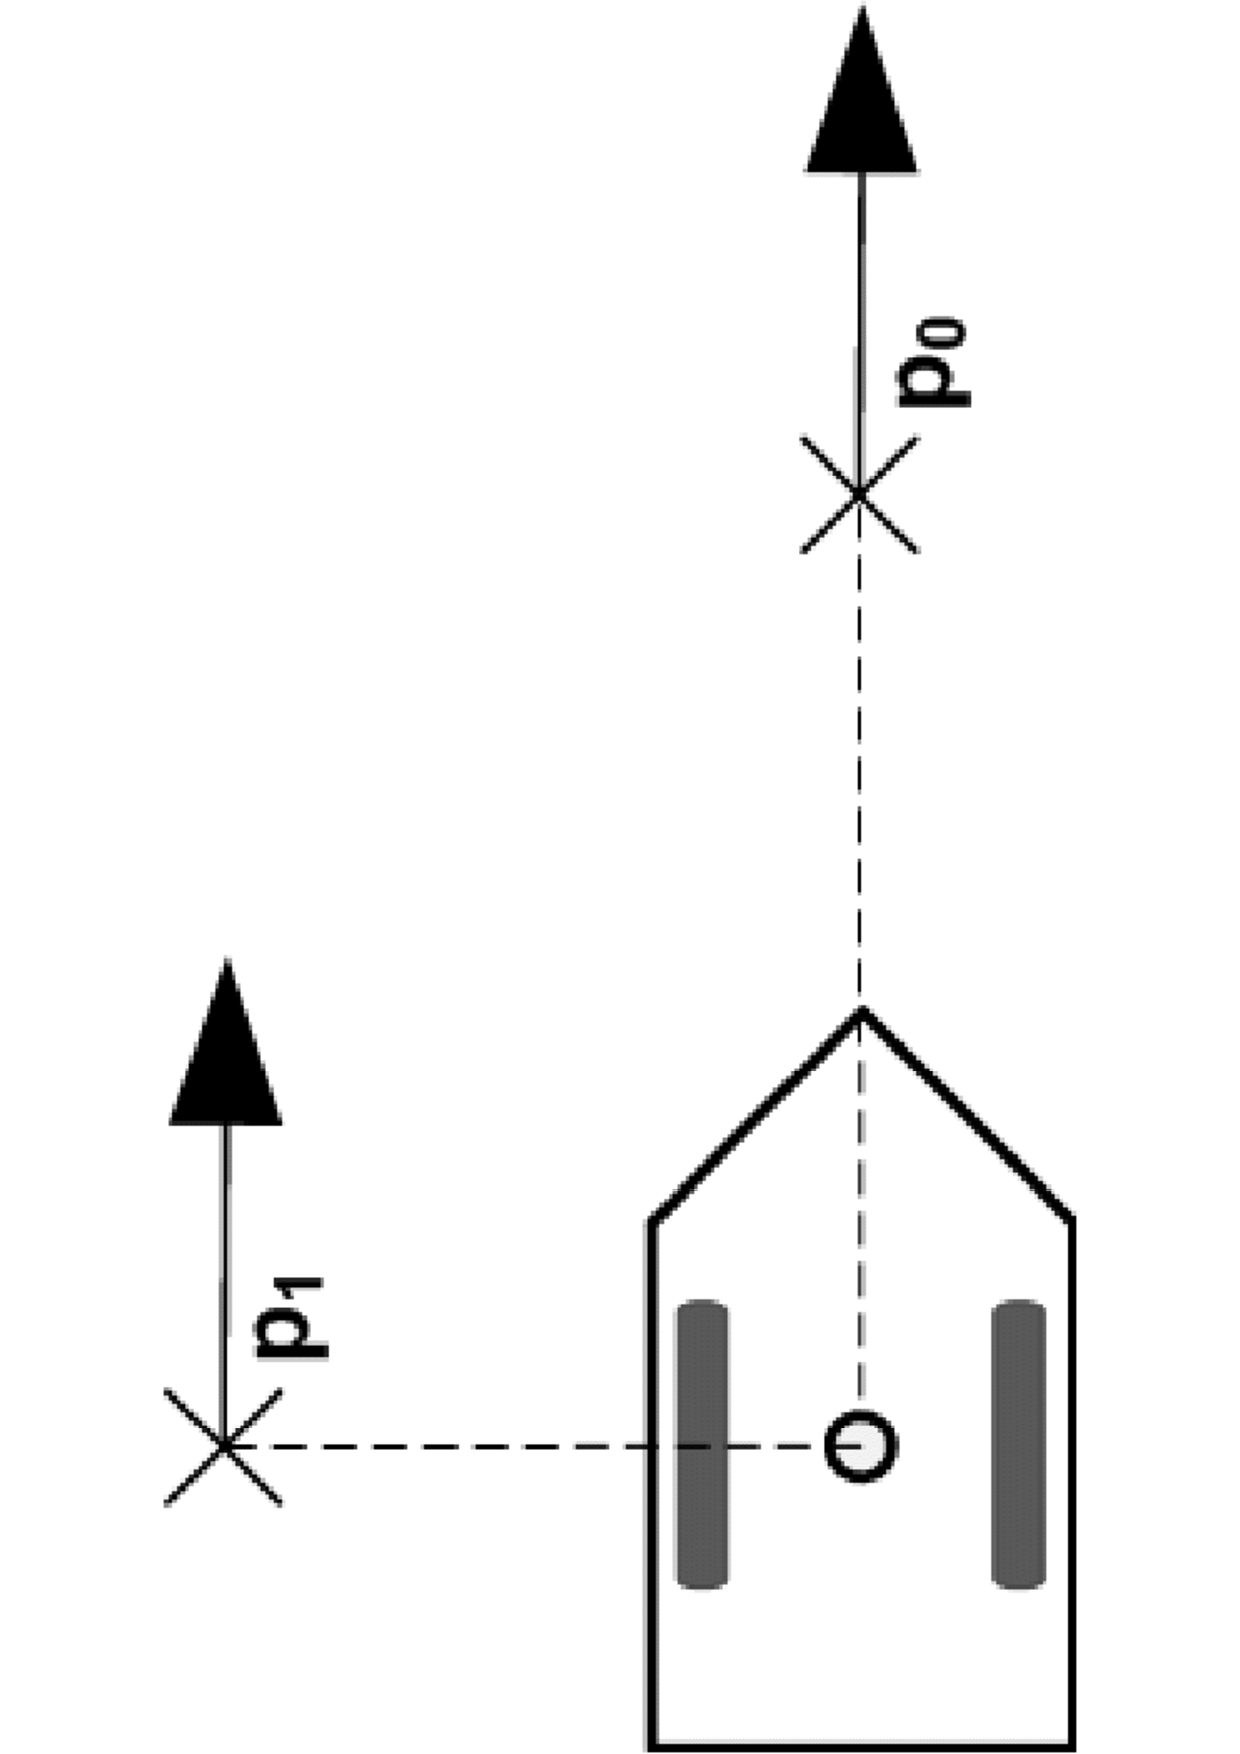
\includegraphics[scale=.2,angle=-90]{figures/rrtfunnel/non-holonomic-vehicle-euclidean-weakness}
  \caption{Consider two poses \(p_0\) and \(p_1\). Although \(p_1\) is nearer
    the robot in Euclidean distance it is harder to get to due to differential
    constraints. In this paper, we propose a directed distance function
    applicable to unicycle- type vehicles, that properly reflects the true
    cost-to-go of the system under the non-holonomic constraint. (figure
    courtesy of \cite{parkFeedbackMotionPlanning2015})}
  \label{fig:non-holonomic-vehicle-euclidean-weakness}
\end{figure}


\subsection{FunnelGraph}

Look at ~\cite{vonasekGlobalMotionPlanning2013} (Algorithm3) for a way of
building an RRT with motion primitives.

\subsection{Funnel-graph}

Even though the \rrtfunnel{} algorithm can work just fine with a collection of
funnels, and simply bruteforcing all funnels at the planning stage, it is
helpful to associate some kind of structure with the collection. Therefore the
funnels will be organised into a graph structure \(\mathcal{F}\) where each
funnel is a edge in the graph, and the inlets and the outlets are vertices. The
funnels also need information about which funnels that they are composable with,
as they may not all be composable with eachother, hence the graph is not
complete.

\begin{figure}
  \centering
  \begin{minipage}[b]{0.4\textwidth}
    
\includegraphics[width=\textwidth]{figures/method/trajectory-sampled}
    \caption{Trajectory sampled 21 times.}
  \end{minipage}
  \hfill
  \begin{minipage}[b]{0.4\textwidth}
    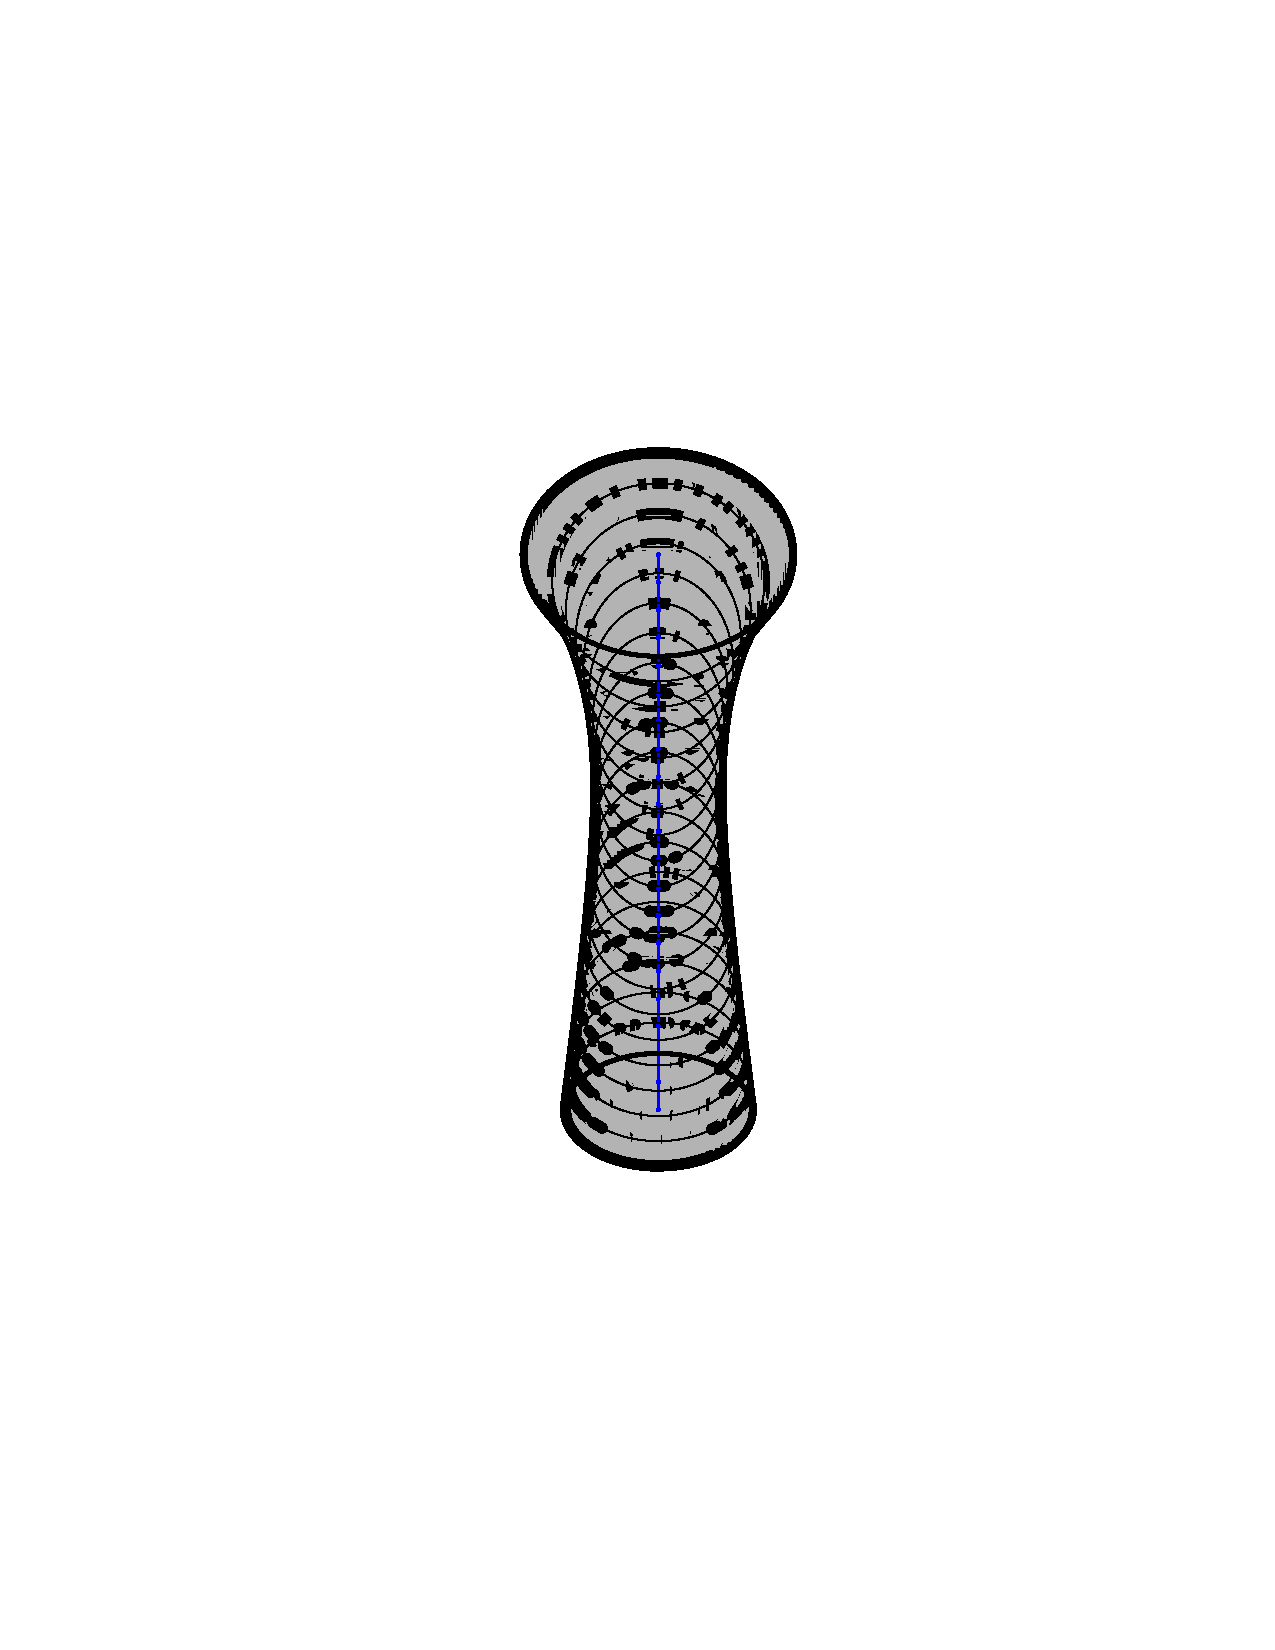
\includegraphics[width=\textwidth]{figures/method/funnel-sampled}
    \caption{The verified trajectory ellipsis overlaid at the sample times.}
  \end{minipage}
\end{figure}

For each funnel, in order to not only be able to compose funnels, but
sub-funnels, which means that at every point of every node in every funnel is
composable with every other sample point in every other funnel has to be
checked. This is summed up more orderly in algorithm
\ref{alg:create-funnel-graph}, where a funnel is a vertice in the graph, and an
ordered pair of funnels \(\left( F_{i}, F_{j} \right)\) is an edge. Composition
of funnels is checked in the same way as in \ref{def:funnel-composition}, and a
\ac{SOS}-program which implements the algorithm can be found in
section~\ref{sec:funnel-composability-program-sos}.

\begin{algorithm}
  \caption{Create Funnel Graph}
  \label{alg:create-funnel-graph}
  \DontPrintSemicolon \SetAlgoNoLine

  \KwIn{\(\mathcal{F}\) -- The basis set of funnels computed around the nominal
    trajectories.} \KwOut{\(\mathcal{G}(\mathcal{F})\) -- Directed graph
    representing the composability of funnels.}

  \ForEach{\(F_{i} \in \mathcal{F}\)} { \ForEach{\(F_{j} \in \mathcal{F}\)} {
      \ForEach{\(t_{k} \in F_{i}\)} { \ForEach{\(t_{l} \in F_{j}\)} {
          \If{\(F_{i}(t_{k}) \subset F_{j}(t_{l})\)} { \(\mathcal{G}
            \leftarrow{} \left( F_{i}(t_{k}), F_{j}(t_{l}) \right)\) }
        }
      }
    }
  }

\end{algorithm}

\subsection{The \rrtfunnel{} algorithm}

With the framework finished, it is time to introduce the formulation of the
\rrtfunnel{} algorithm itself. The \rrtfunnel{} algorithm is a modified \ac{RRT}
algorithm which employs the precomputed funnels as motion primitives for its
expansion operator, and pseudocode for its definition can be found
in~\ref{alg:rrtfunnel}.

\begin{algorithm}
  \caption{Check funnel composability}
  \label{alg:create-funnel-graph}
  \DontPrintSemicolon \SetAlgoNoLine

  \KwIn{\(\mathcal{F}\) -- The basis set of funnels computed around the nominal
    trajectories.} \KwOut{\(\mathcal{G}(\mathcal{F})\) -- Directed graph
    representing the composability of funnels.}

  \ForEach{\(F_{i} \in \mathcal{F}\)} { \ForEach{\(F_{j} \in \mathcal{F}\)} {
      \If{\(F_{i}(t_{0}) \subset F_{j}(t_{end})\)} { \(\mathcal{G} \leftarrow{}
        \left( F_{i}(t_{0}), F_{j}(t_{end}) \right)\) } \; }\; }\;

\end{algorithm}

\begin{figure}
  \centering 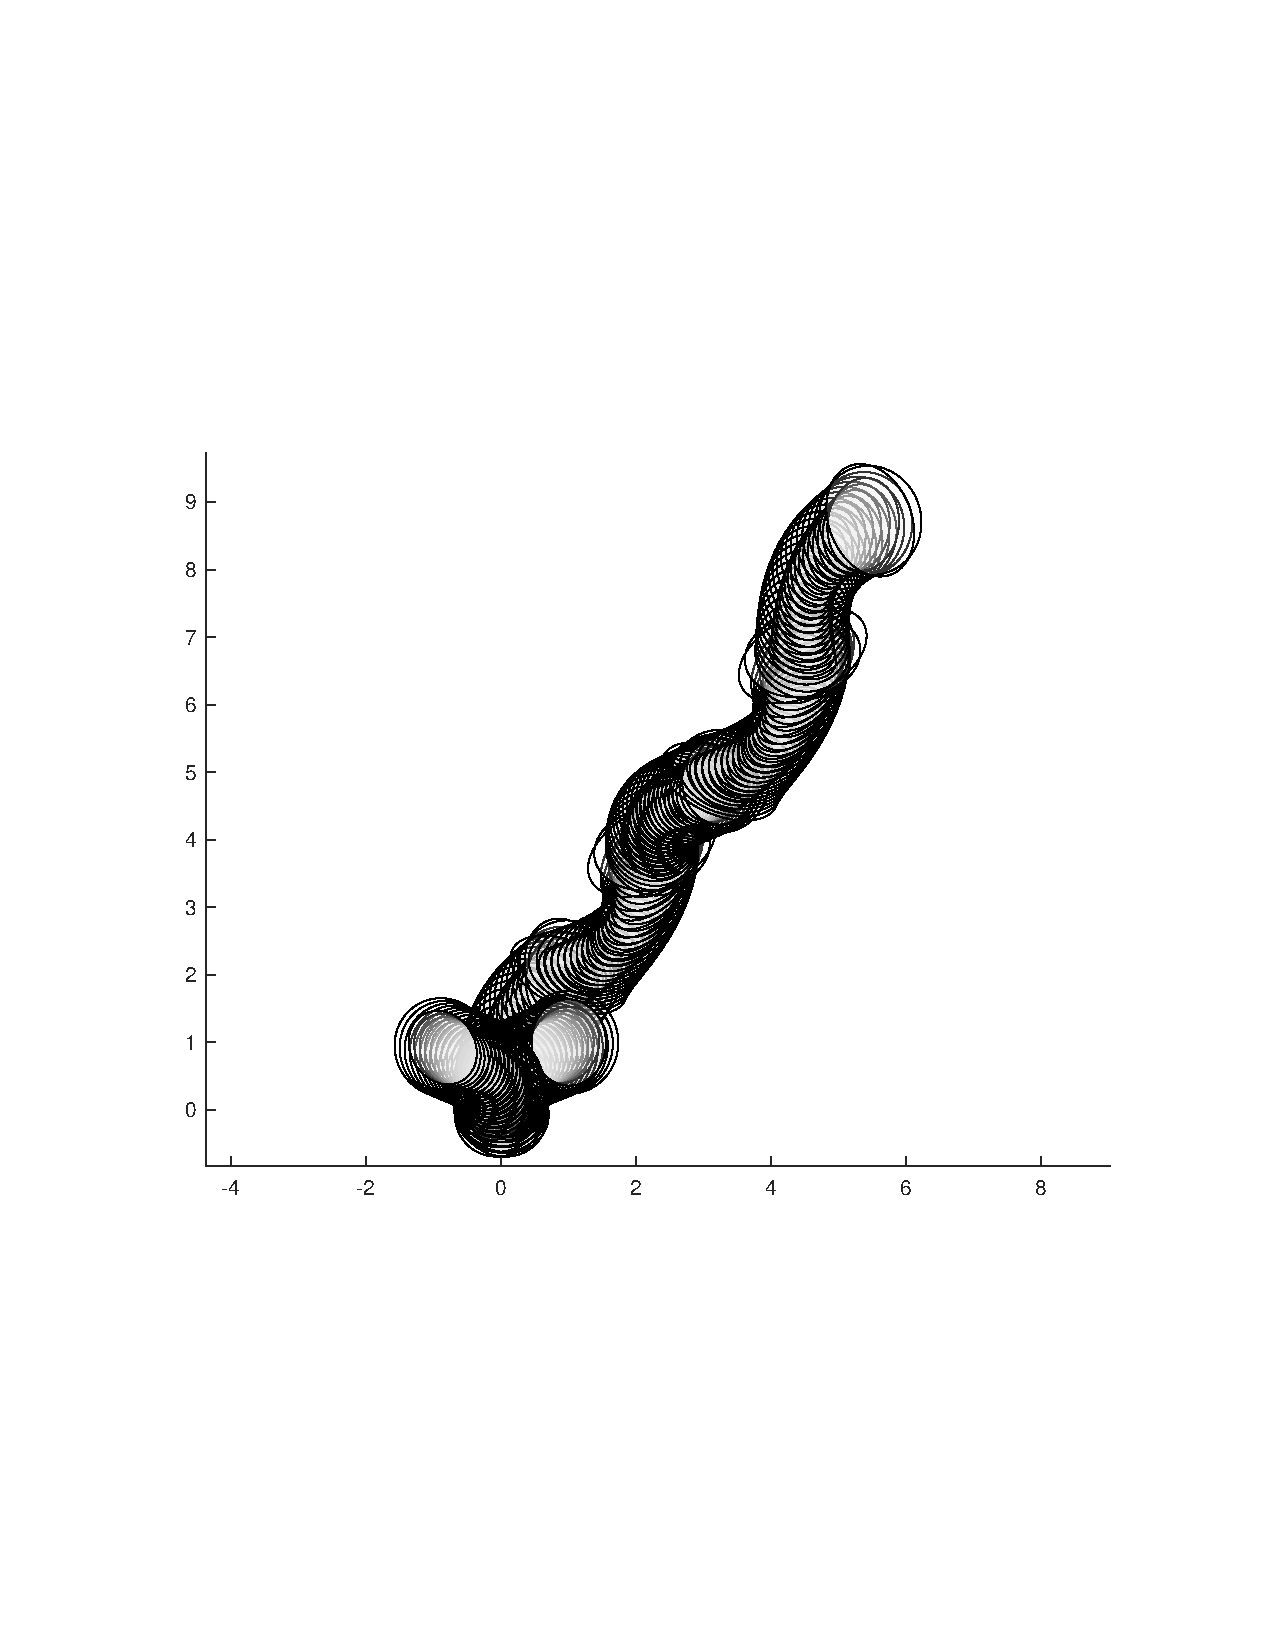
\includegraphics[scale=.5]{figures/method/funnel-tree}
  \caption{Picutred: A tree of funnels built by the \rrtfunnel{} algorithm.}
\end{figure}

The \rrtfunnel{} algorithm is defined as

\begin{algorithm}[H]
  \caption{\rrtfunnel{} algorithm}
  \label{alg:rrtfunnel}
  \DontPrintSemicolon

  \KwIn{Initial configuration, \(q_0\)} \KwOut{\textit{RRT}-Funnel-graph
    \(\mathcal{G}\)}

  \SetKwFunction{RandConf}{Sample\_Random\_Configuration}
  \SetKwFunction{NearestVertex}{Find\_Nearest\_Vertex}
  \SetKwFunction{Extend}{Extend} \SetKwFunction{AddVertex}{add\_vertex}
  \SetKwFunction{AddEdge}{add\_edge}
  \SetKwFunction{ExtractBranch}{Extract\_Branch}
  \SetKwFunction{TestUncertainFunnels}{Test\_Uncertain\_Funnels}
  \SetKwFunction{BuildComposabilityMatrix}{Build\_Composability\_Matrix}

  \TestUncertainFunnels{} \;
  \BuildComposabilityMatrix{}

  \(\mathcal{G}.init(q_0)\) \For{\(i \leftarrow 1\) \KwTo \(k\)}{ \(q_{rand}
    \leftarrow \) \RandConf{} \; \(q_{near} \leftarrow \)
    \NearestVertex{\(q_{rand}, \mathcal{G}\)}\; \(q_{new} \leftarrow \)
    \Extend{\(q_{near}, q_{rand} \)}\; \If{\(q_{new} \in
      \modelconfigurationspacefree{} \) } {
      \(\mathcal{G}\).\AddVertex{\(q_{new}\)}\;
      \(\mathcal{G}\).\AddEdge{\(q_{near}, q_{new}\)} \; \If{\(q_{new} \in
        \mathcal{X}_{goal}\)}{ return \ExtractBranch{\(\mathcal{G}\)} \; }\; } }

  \SetKwProg{Def}{def}{:}{end} \Def{\RandConf{}}{ return 0\; }
  \Def{\TestUncertainFunnels{}}{ return 0\; }
  \Def{\BuildComposabilityMatrix{}}{ return 0\; }
  \Def{\NearestVertex{\(q_{rand}, \mathcal{G}\)}}{ return 0\; }
  \Def{\Extend{\(q_{near}, q_{rand} \)}}{ return 0\; }

  \Def{\ExtractBranch{}}{ return 0\; }

\end{algorithm}

\subsection{Special maneuvers}

The algorithm incorporates room for two special maneuvers.

\subsubsection{The identity funnel for starting the simulation fresh}

The identity funnel is an empty placeholder for the start node of the graph,
that does no transformations on the model at all, and thus can be seen as the
identity element in the funnel space, or rather, the identity funnel.

\subsubsection{Emergency maneuver}

If the vehicle is to leave the verified funnel at execution time -- this could
happen for any number of reasons, such as unmodelled uncertainties -- the
vehicle should execute the emergency maneuver, which in this case is a simple
stop maneuver. Since the model employed is a simple first order model, a halt
will happen momentarirly. Still, an emergency maneuver can be any sort of 'safe'
maneuver for the model at hand -- such as a loiter circle for an airplane, or
idling at one place for a quadcopter.

\subsection{Collision checking}


    \part{Results}
    \chapter{Experiments}

The \rrtfunnel{} algorithm developed this far will now be tested in a simulation
experiment where a simple unicycle model of a car will be set to traverse a
small strip of forest. The simulation environment can be seen
in figure~\ref{fig:simulated-forest}, where the vehicle starts at one end of the
obstacle forest, and is set to traverse the strip of forest and reach any
\((x,y)\) position in a circle of radius five surrounding the endpoint thirty
five meters ahead.

\begin{figure}
  \centering
  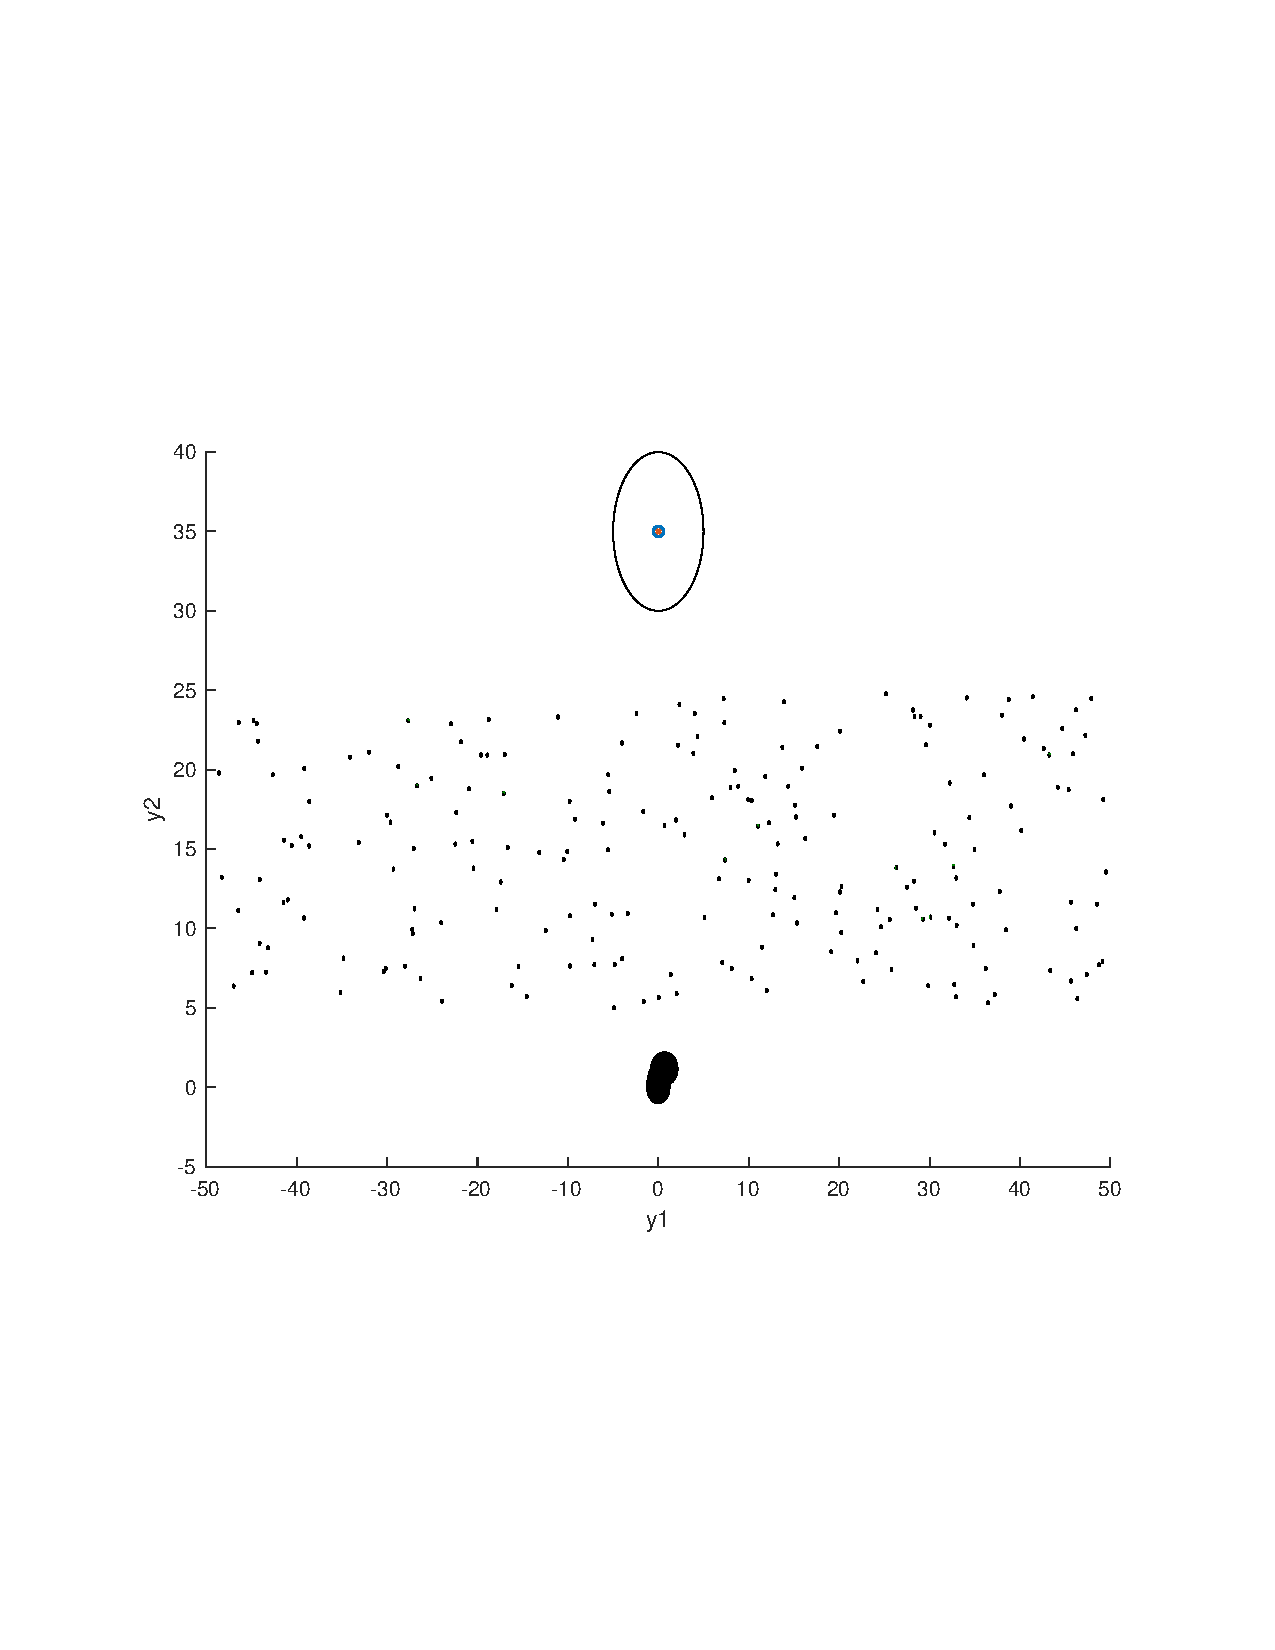
\includegraphics[scale=.5]{figures/experiments/simulated-forest}
  \caption{The experiment environment.}
  \label{fig:simulated-forest}
\end{figure}

\subsection{Generating the obstacle forest (Poisson processes)}
\label{sec:Poisson-Process}

In order to generate the obstacle field for the experiments, which is to
resemble a forest, a \textit{spatial Poisson process} is employed. Poisson
processes are used to model random configurations of points in
space'~\cite{kroeseSpatialProcessGeneration}, and hence are well suited for
generating a simulated forest. For the experiments below, a forest will be the
realization of a spatial Poisson process on \(\R^2\).

A few key parameters of the Poisson process has to be set for use in the
experiments below. Firstly, \(\lambda\) is the intensity of the spatial process.
For these experiments, the intensity will be held constant, and the process is
therefore homogeneous, as it does not vary with the position in space. One
interesting configuration could be to vary the intensity as the radius from
origo, and hence the difficulty in traversing the terrain would increase with
the distance travelled. However, the constant intensity setting was chosen to
keep things simple and uniform.

The algorithm for realizing a random Poisson measure~\ref{def:Poisson-def} is
taken from~\cite[Definition 1.1.1,p~34]{kroeseSpatialProcessGeneration}.

\begin{definition}[Generating a Poisson random measure]
  \label{def:Poisson-def}
  \begin{enumerate}
  \item Generate a Poisson random variable \(N ~ Poi(\mu(E))\).
  \item Draw \(X_1,X_2,\ldots,X_N ~ g\), where \(g(x) \lambda(x)/ \mu(E)\).
  \end{enumerate}
\end{definition}
where \(E\) is the set over which the points should be generated, and the
\textit{pdf} \(g(x_1, x_2) = \lambda(x)/\mu(E)\). Finally, \(\mu(E)\) is defined
as
\[
  \mu(E) = \int_{E} \lambda(x) dx.
\]

For the experiments the set \(E\) will be a square defined as
\[
  E = [-\alpha, \alpha]^2
\]
the density of the generated forest \(\lambda\) will be set to
\[
  \lambda = 0.1
\]
of which the resultant forest on a \(20 \times 20\) grid can be seen in
figure~\ref{fig:poisson009}.

\begin{figure}
  \centering
  \begin{minipage}[b]{0.4\textwidth}
    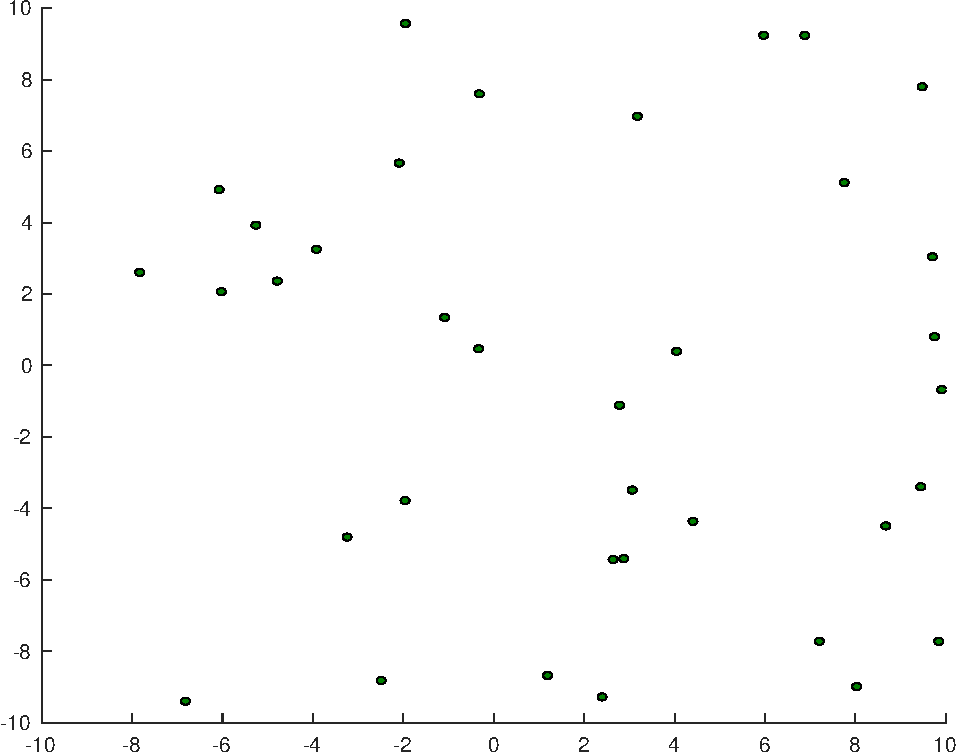
\includegraphics[width=\textwidth]{figures/experiments/poisson009}
    \caption{The resultant forest generated by a spatial Poisson process with
      intensity \(\lambda = 0.1\)}
    \label{fig:poisson009}
  \end{minipage}
  \begin{minipage}[b]{0.4\textwidth}
    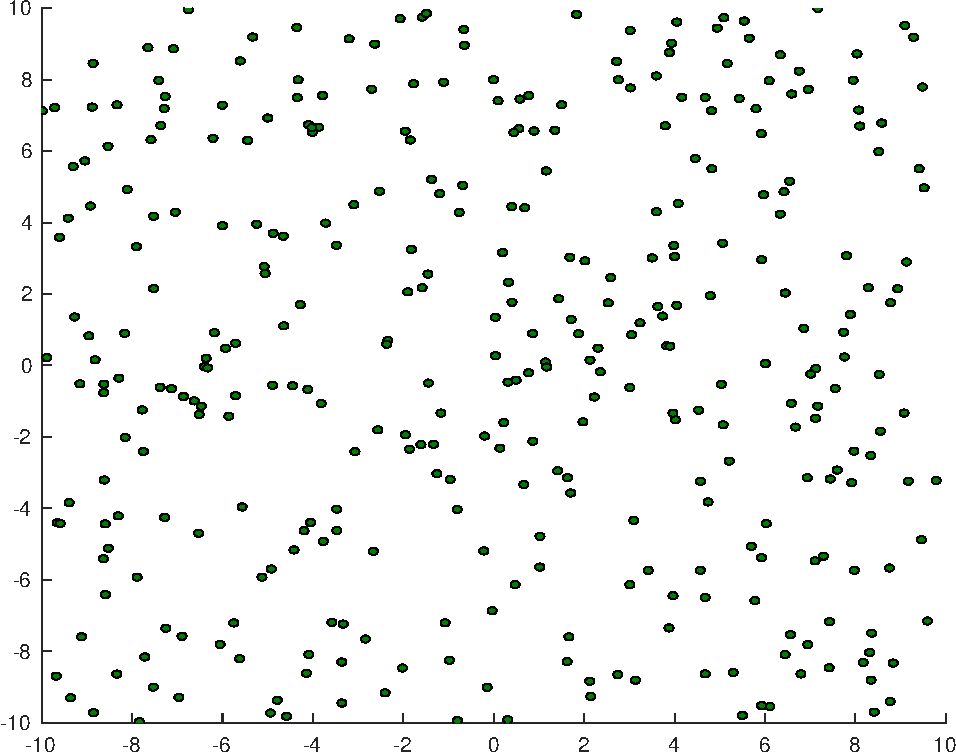
\includegraphics[width=\textwidth]{figures/experiments/poisson09}
    \caption{The resultant forest generated by a spatial Poisson process with
      intensity \(\lambda = 0.9\)}
    \label{fig:poisson09}
  \end{minipage}
\end{figure}

\subsection{Deciding upon the size of the vehicle and the obstacles}

The funnels generated thus far is created from a point model of the vehicle, and
its dynamics. If the grid that the simulations are run on are set to have an
increment of a meter, then the funnels from the basic set are given a velocity
of \([v(t)] = \si{m.s^{-1}}\), \([\theta] = \si{\radian\per\second}\), and
\([\dot{\theta}] = \si{\radian\per\second\per\second}\), where \([\cdot]\) is
the unit operator. The size of the vehicle is arbitrary, and can be chosen
freely, but if it is imagined as a radio controlled car, with a speed of
\(10\si{m.s^{-1}}\), then a size of \(30 \times 20 \si{\centi\metre} \) keeps
everything within the realm of a normal radio controlled car and its
capabilities. The mass is not relevant for our first order dynamics, but still
the vehicle is assigned a mass of \(1 \si{\kilo}\), so that the translation of
the model dynamics is not irrelevant. A figure of the vehicle can be seen
in figure~\ref{fig:radio-vehicle}.

\begin{figure}
  \centering
  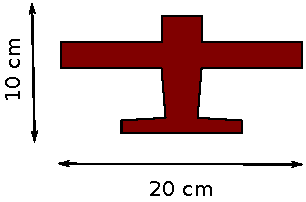
\includegraphics[scale=.3]{figures/experiments/radio-vehicle-model}
  \caption{The vehicle employed in the simulation experiments.}
  \label{fig:radio-vehicle}
\end{figure}

\subsection{Expanding the size of the funnel by the size of the simulated
  vehicle}

The size of the vehicle in the original model is a single point, and as such,
the vehicle model with a size is not accounted for in the funnels prior to
running the simulations. Therefore the funnels have to be expanded in order for
them to accomodate the necessary robustness guarantees that are expected from
the algorithm. However, the size of the vehicle only affects the size of the
funnel ellipsis projected down into the xy-plane. Therefore first getting the
projected size of the funnel, where \(P \colon \R^4 \rightarrow \R^2\) is a
projection map with a projection matrix
\[
  P =
  \begin{bmatrix}
    I_{2 \times 2} & \mathbf{0}_{2 \times 2} \\
  \end{bmatrix}
\]
such that for the projected ellipsoid
\[
  \mathcal{E}_{p} = \set{\bar{x} \in \R^{2} \mid {\bar{x}}^{T}S_{k}^{(p)}\bar{x}
    \leq 1}
\]
and
\[
  S_{k}^{(p)} = \left( PS_{k}^{-1}P^T \right)^{-1}
\]
and \(\mathcal{E}_{p}\) is the projected set of the ellipsoid projected down
into the xy-plane~\cite{majumdarFunnelLibrariesRealtime2017}. In general an
ellipse centered at the origin is a linear transformation of the unit
circle~\cite{lay2005linear}. Exploiting this fact, expanding the radius of the
circle to encompass the vehicle model. Also taking into account that the matrix
\(S_{k}\) is \textit{Positive semidefinite}, and hence can be cholezky
factorized~\cite{lay2005linear}. The expanded ellipsis (which now contains all
the possible states of the vehicle model) is:

\begin{align*}
  S_{k}^{\mathcal{P}} &= R^{T}R \\
  \mathcal{C} &= \set{y \in \R^2 \mid y^{T}y \leq 1 + r_{vehicle}} \\
  S_{k}^{p'} &= R^{-1}y \\
\end{align*}

where \(S_{k}^{'}\) is the ellipsoid which contains the volume of the vehicle
for all verfied states in the funnel. A picture of the initial funnel and the
funnel expanded around the vehicle model can be seen
in figure~\ref{fig:expanded-funnel} and figure~\ref{fig:expanded-and-unexpanded}.

\begin{figure}
  \centering 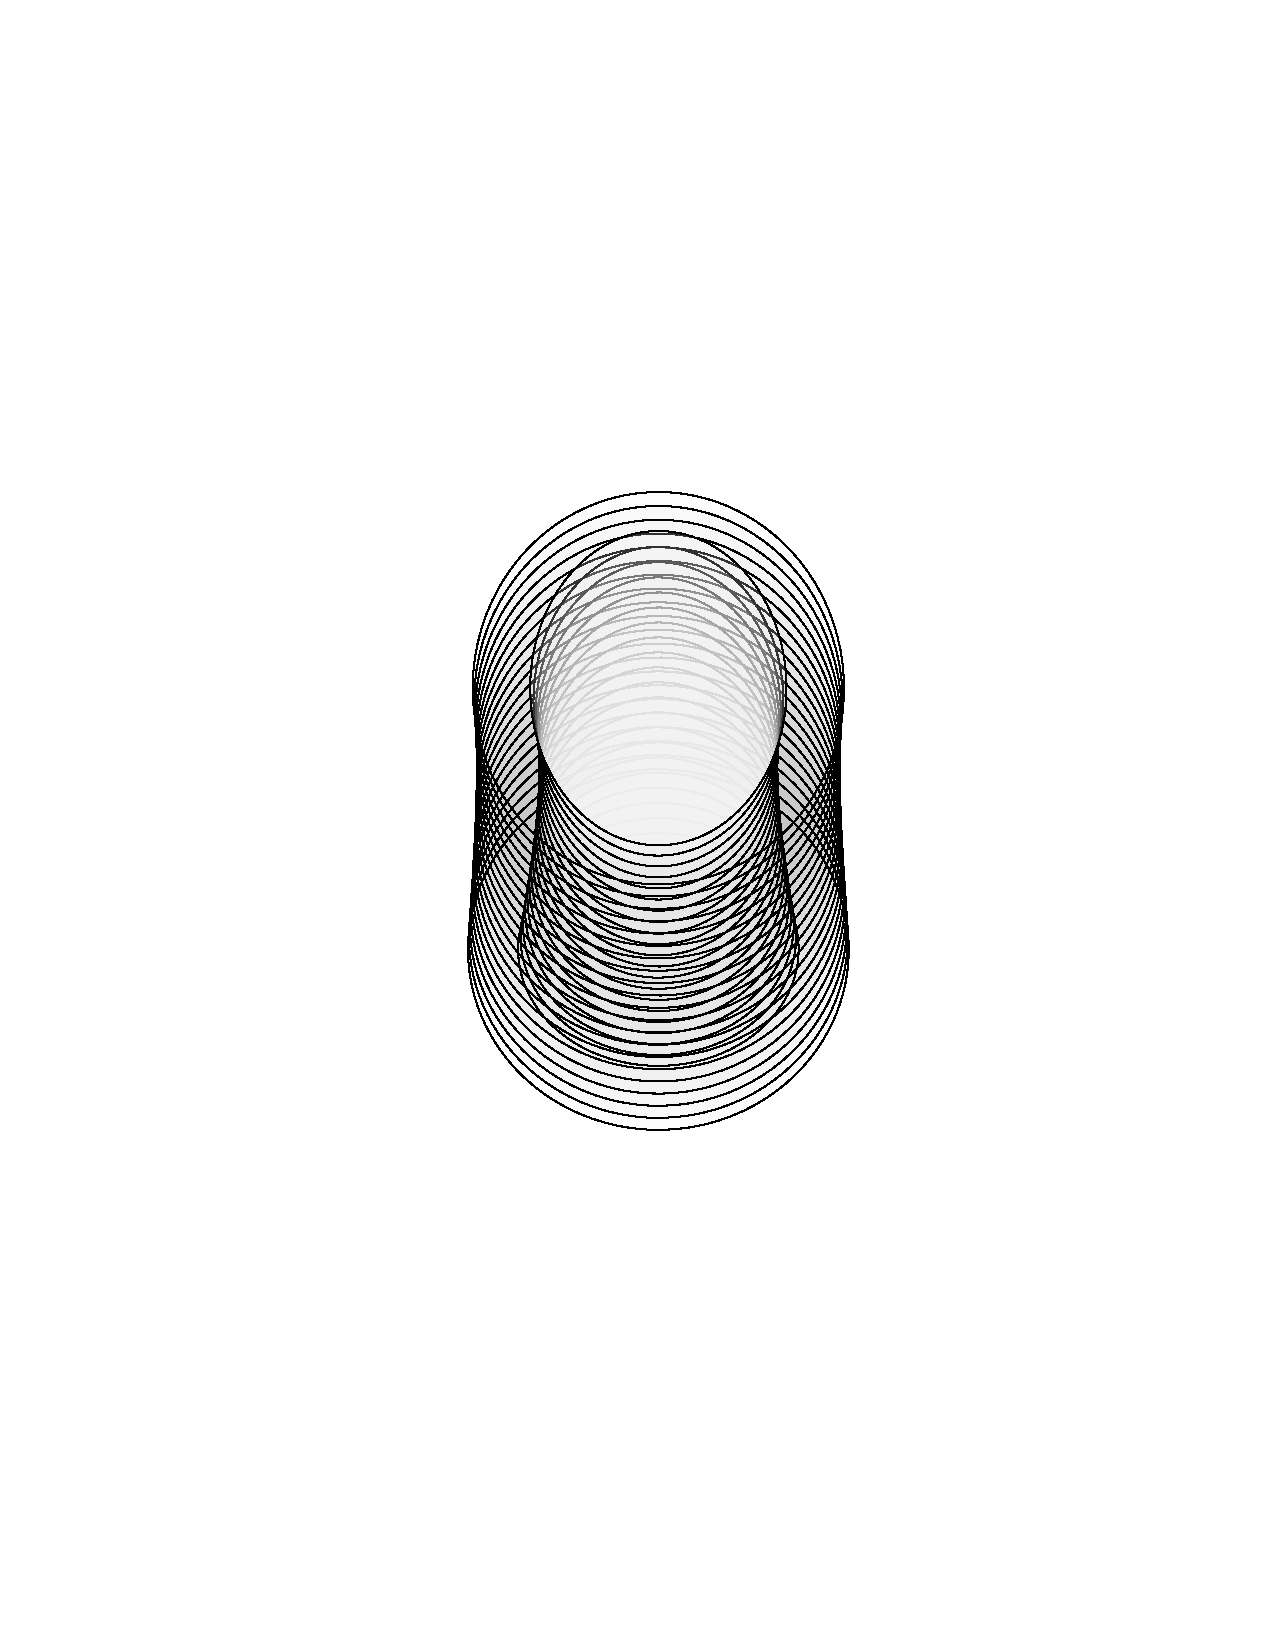
\includegraphics[clip, trim=6cm 8cm 6cm 8cm,
  scale=.5]{figures/method/expanded-funnel}
  \caption{The original funnel created from the point model, with a funnel
    expanded by a radius of 0.2 surrounding it.}
  \label{fig:expanded-funnel}
\end{figure}

\begin{figure}
  \centering
  \begin{minipage}{0.4\textwidth}
    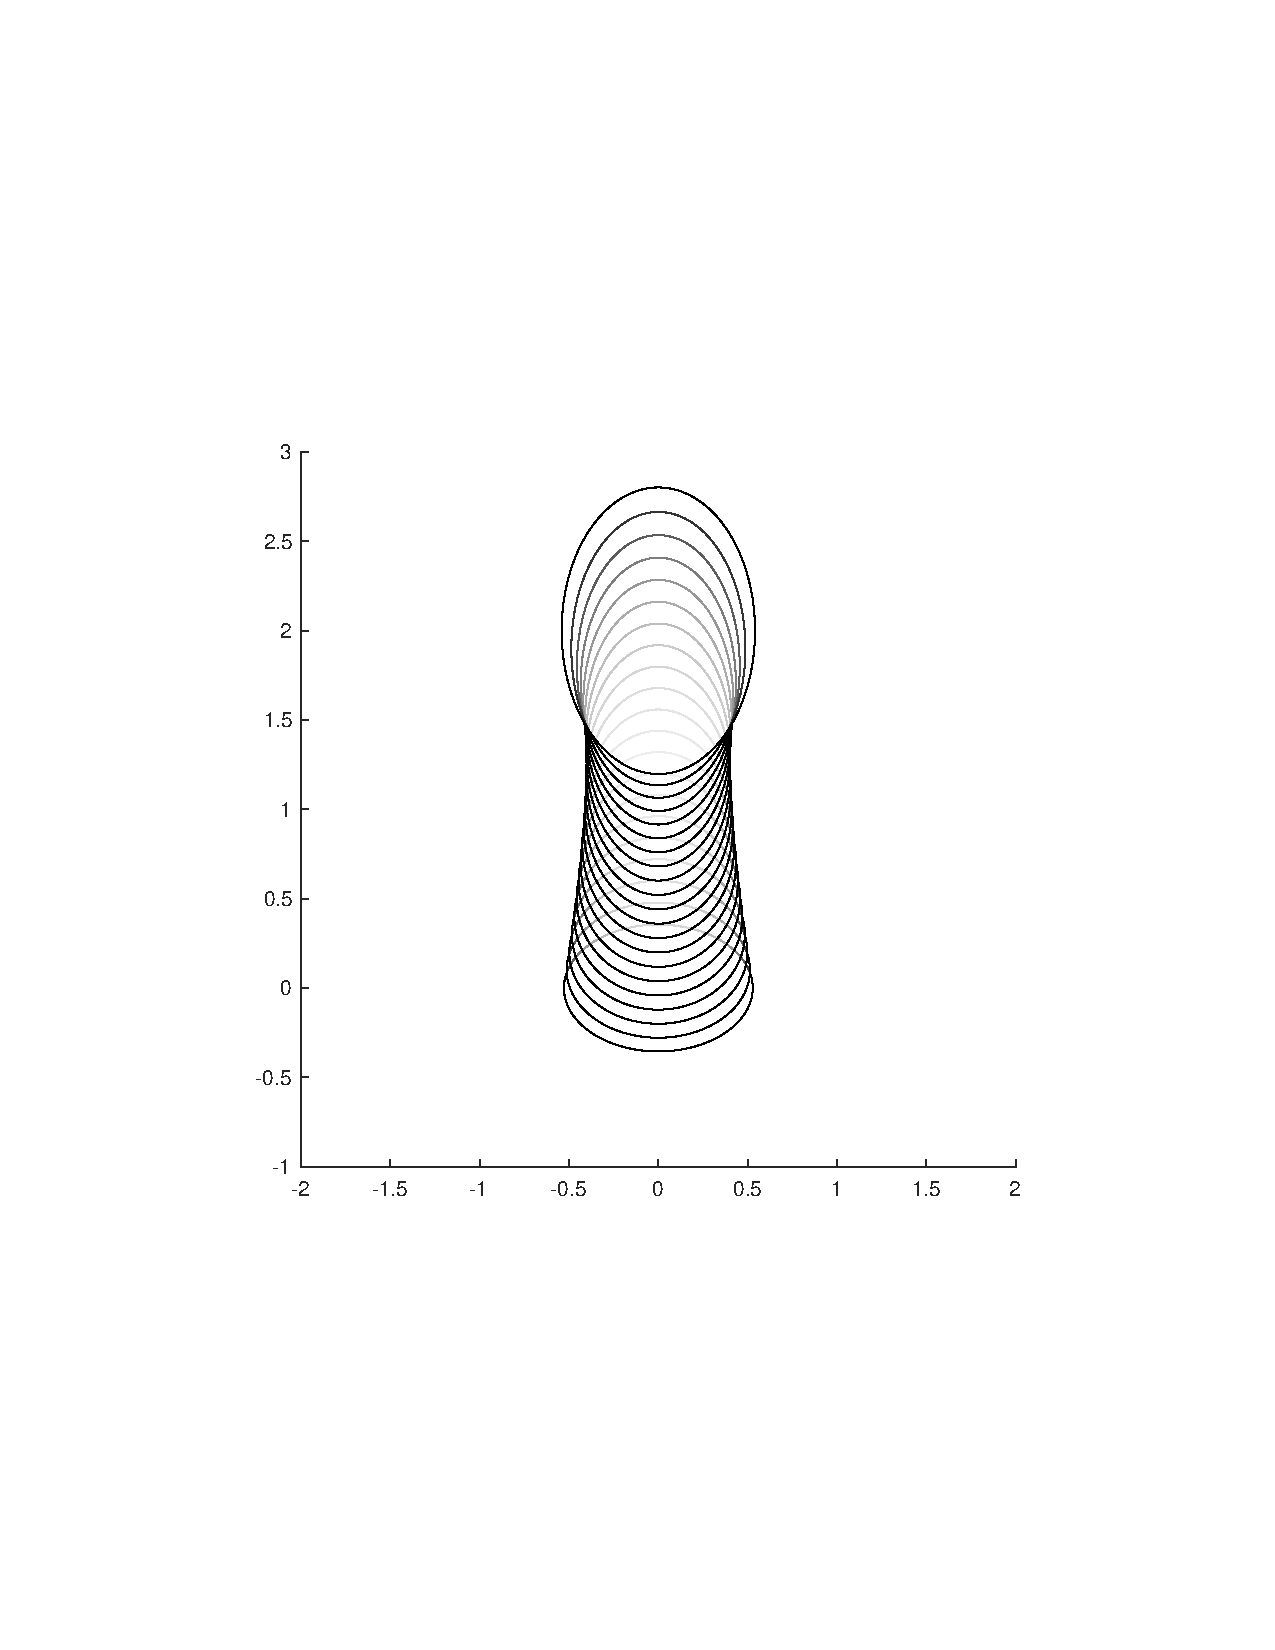
\includegraphics[scale=.3]{figures/method/unexpanded-funnel}
    \caption{The funnel around a straight trajector for the point model.}
  \end{minipage}
  \begin{minipage}{0.4\textwidth}
    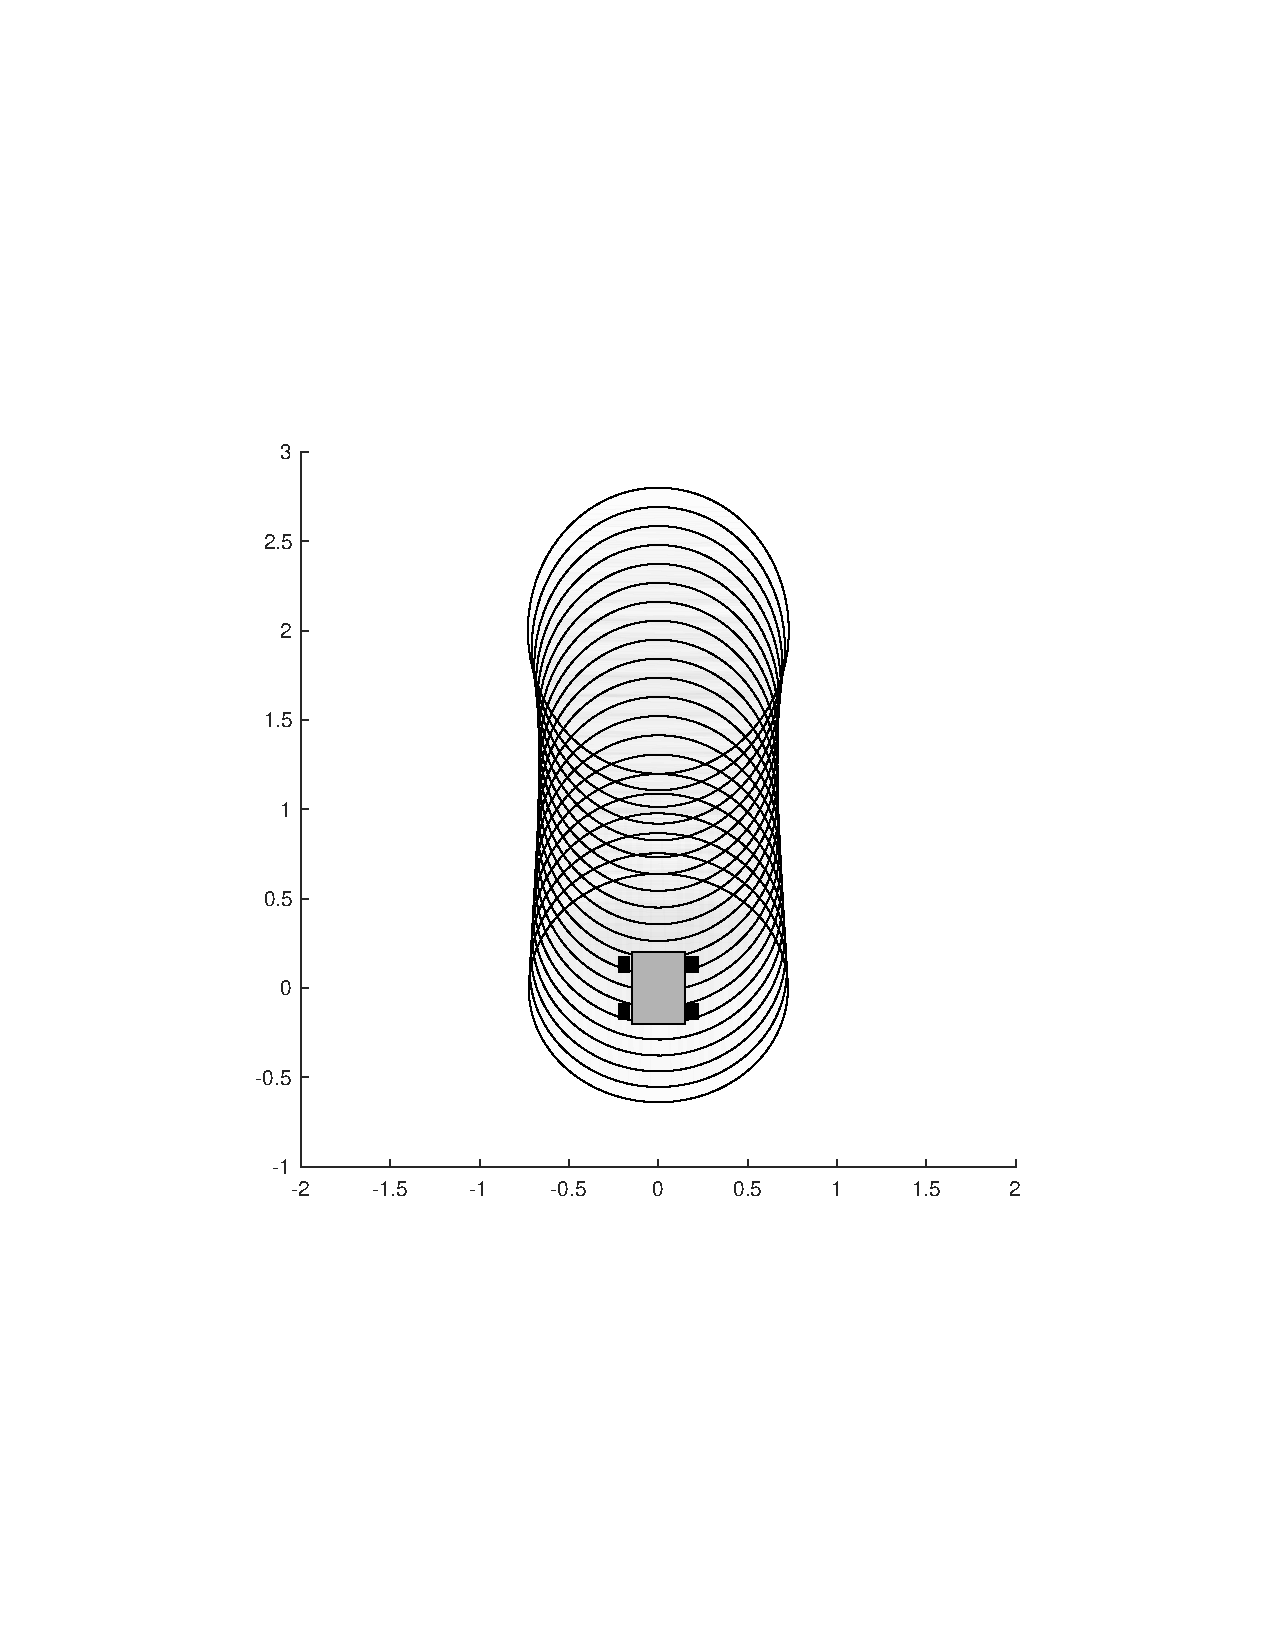
\includegraphics[scale=.3]{figures/method/expanded-funnel-with-car}
    \caption{The funnel around a straight trajector for the point model.}
  \end{minipage}
  \caption{Pictured: An unexpanded and a funnel expanded by the size of the
    simulation vehicle.}
  \label{fig:expanded-and-unexpanded}
\end{figure}

\subsection{The initial motion primitive set}

The basis set of motion primitives should be small, yet cover enough of the
finer movements of the vehicle so that the motion of the vehicle can be near
continuous when composed together. Thus in order to generate a 'dense' set of
motion primitives the algorithm~\ref{alg:initial-motion-primitives-generation}
is employed to generate points along the arch of a circle with \(N\) different
radii.

\begin{algorithm}[H]
  \label{alg:initial-motion-primitives-generation}
  \caption{Generating the initial motion primitives (TODO) - update with the new
    primitives!}
  \DontPrintSemicolon \SetAlgoNoLine

  \KwIn{
    \(n\) - Number of points along the arch \\
    \(r_{0}\) - Initial radius \\
    \(r_{f}\) - Final radius \\
    \(s\) - Stepsize (\(r_{n+1} = r_{n} + s\)) } \KwOut{\(\mathbf{X}\) -
    Endpoints matrix for the trajectory generator}

  \(\theta_{0} = \pi\) \;

  \For{\(r_{k+1} = r_{k} + s\)}{ \(\theta_{j} = \frac{\theta{0}}{2r}\) \;
    \(\theta_{stepsize} = \frac{\theta{j}}{(n-1)/2}\) \; \(\mathbf{X} \leftarrow
    (r_{k+1}, \theta=0)\) \; \For{\(i = 1 \) \KwTo \(\frac{n-1}{2}\)}{
      \(\theta_{ki} = i*\theta_{stepsize}\) \; \(\mathbf{X} \leftarrow (r, \pm
      \theta_{ki})\) \; }\; }\;
\end{algorithm}

The initial trajectories employed in the experiments can be seen in
figure~\ref{fig:intial-trajectories-exp}, and the projected funnels overlaid a
sample in figure~\ref{fig:sample-funnel-overlay}.

\begin{figure}
  \centering
  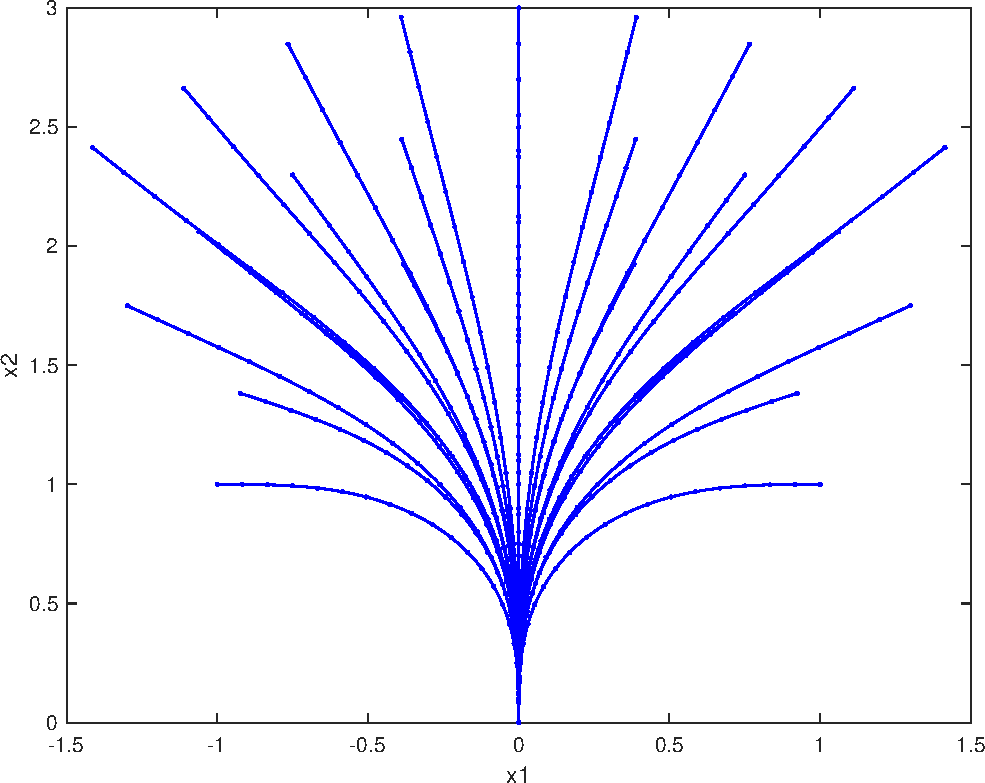
\includegraphics[scale=.5]{figures/experiments/initial-trajectories}
  \caption{The initial trajectories used in the \rrtfunnel{} algorithm.}
  \label{fig:intial-trajectories-exp}
\end{figure}

\begin{figure}
  \centering
  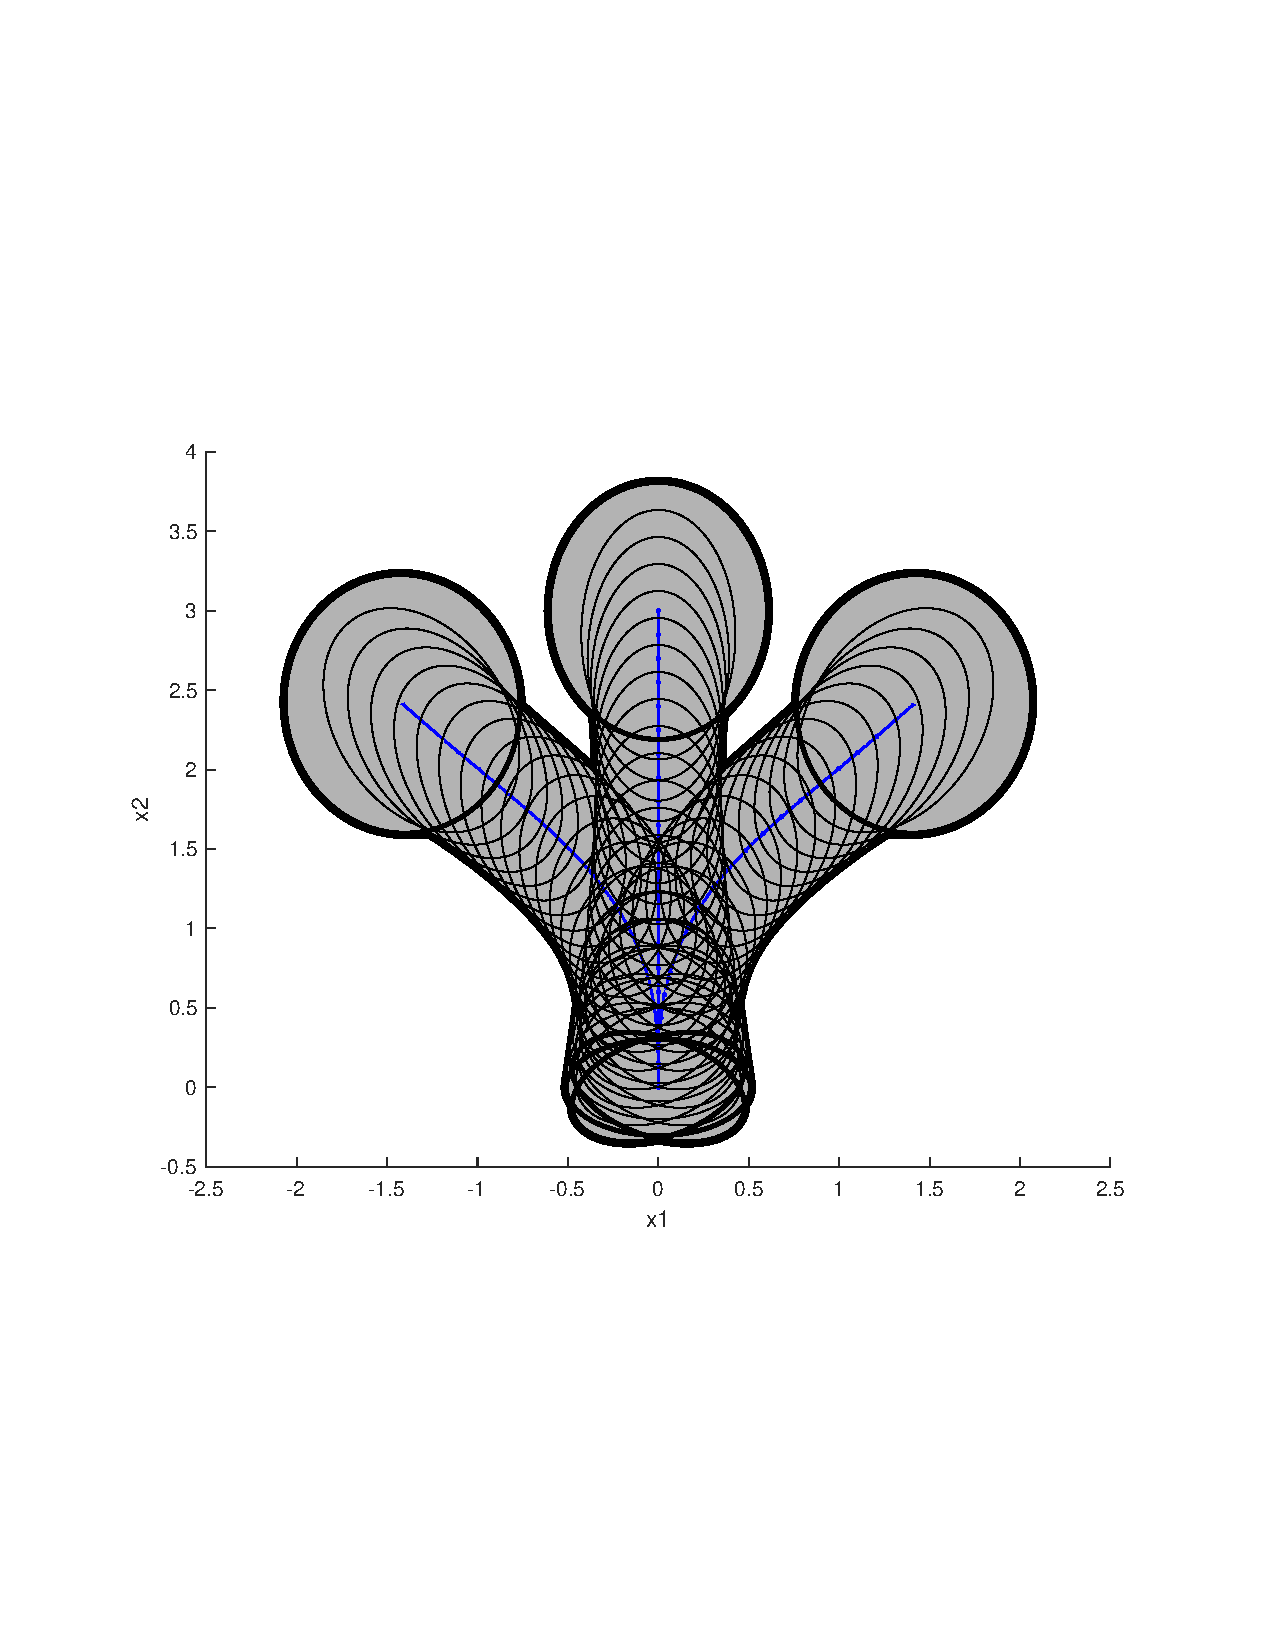
\includegraphics[scale=.5]{figures/experiments/sample-funnel-overlay}
  \caption{Three funnels from the initial trajectories with the projected
    funnels overlaid.}
  \label{fig:sample-funnel-overlay}
\end{figure}

\subsection{LQR cost matrices}

Although the focus of this thesis is not on fine-tuning the controller, some
amount of effort has to go into getting the cost parameters acceptable, so that
the funnels actually converge. In general the strategy is penalizing the
vehicle's distance from the nominal path in \((x,y,\theta)\), and not caring for
the energy expended by the control input. Thus path divergence is penalized
hard, and input divergence is not.

More specifically the cost matrices employed are
\begin{align*}
  R &= 0.01 \\
  Q &= \begin{bmatrix}
    40 & 0 & 0 & 0 \\
    0 & 40 & 0 & 0 \\
    0 & 0 & 40 & 0 \\
    0 & 0 & 0 & 4 \\
  \end{bmatrix}
  \\
  Q_{f} &=
          2\times
  \begin{bmatrix}
    1 & 0 & 0 & 0 \\
    0 & 1.5 & 0 & 0 \\
    0 & 0 & 1 & 0 \\
    0 & 0 & 0 & 1 \\
  \end{bmatrix}
\\
\end{align*}
where the control input is only penalized \(\frac{1}{10}\)th of the other
variables.

\subsection{Making sure that the vehicle stays within the funnels during execution}

During the execution of the \rrtfunnel{} algorithm the planner keeps track of
the funnel during execution, and aborts the simulation with the emergency
maneuver if the vehicle happens to leave one of the funnels at runtime. This
will be counted in the experiments as a collision on the part of the
\rrtfunnel{} algorithm.

\subsection{Show the funnel inlets and outlets from the funnel computations}

Unfortunately, the funnels do not compose, and the composition checking of the
algorithm has to be left out. This is because the controller has no influence on
the speed of the vehicle, and hence there is no way to make the system converge
in the direction of speed as examplified in the figure~\ref{fig:funnel-conv}.

\begin{figure}
  \centering
  \begin{subfigure}[b]{0.4\textwidth}
    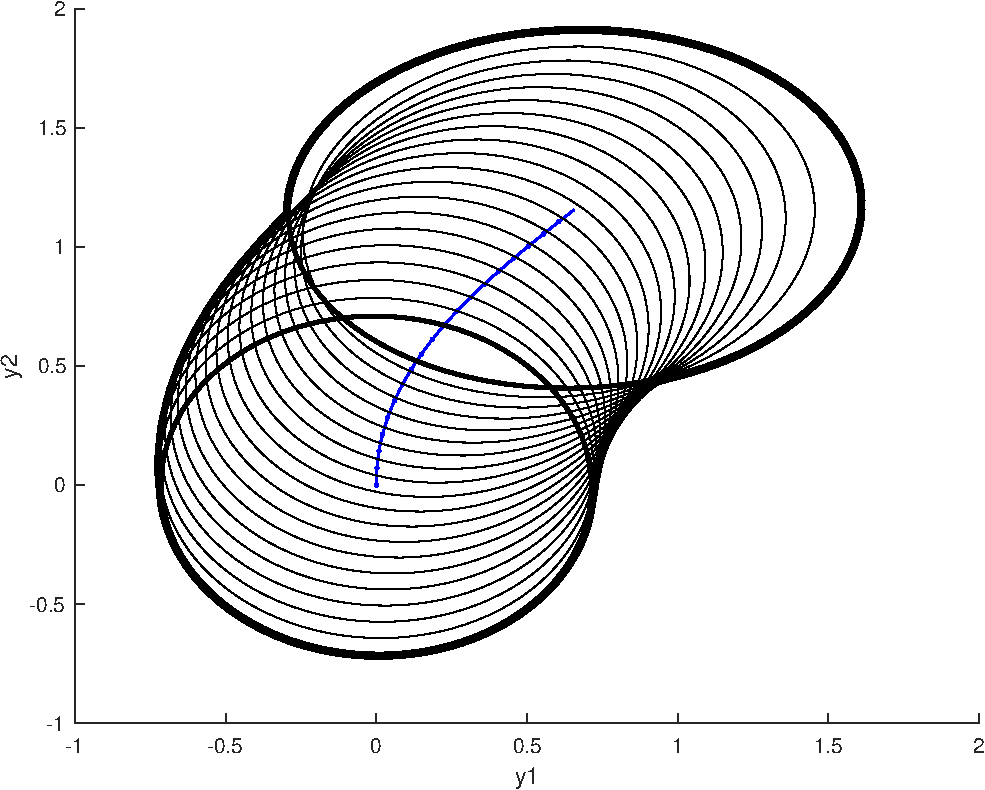
\includegraphics[width=\textwidth]{figures/experiments/sos-calculation}
  \end{subfigure}
  \quad
  \begin{subfigure}[b]{0.4\textwidth}
    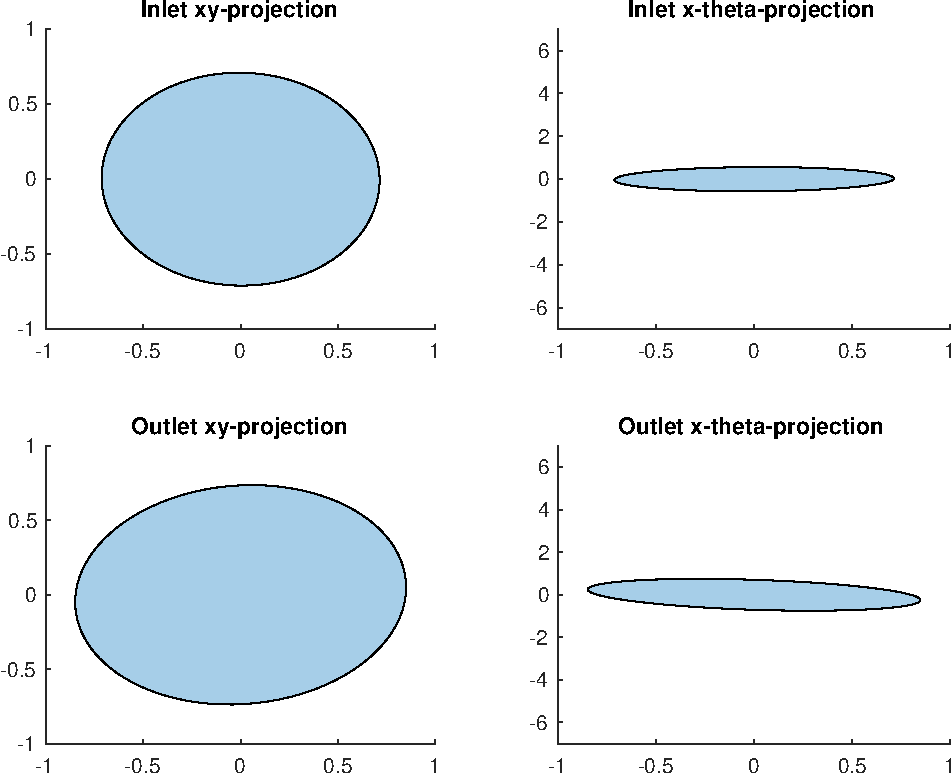
\includegraphics[width=\textwidth]{figures/experiments/sos-calculation-inlet-outlet}
  \end{subfigure}
  \caption{Pictures: A slice of the inlet and the outlet ellipsis in the x-y and
  x-theta dimensions.}
\end{figure}

\section{Experiments}

The experiments will run the \rrtfunnel{} against a benchmark regular RRT
planner with the motion primitive set pictured
in figure~\ref{fig:intial-trajectories-exp} on the forest traversal problem pictured
in figure~\ref{fig:simulated-forest}.

The benchmarkplanner is an \ac{RRT} algorithm
using the same motion primitive set as the \rrtfunnel{} algorithm, with the same
\ac{LQR} controller, and the same distance metric. The difference is that it
does not take uncertainty into account, and instead maximizes the distance to
the nearest obstacle as the extension operator \ie{}
\begin{equation}
  \max_{i}\min_{t,j}(x_{i}(t), o_{j})
\end{equation}
where \(x_{i}(t) \in \mathcal{T}\), is a trajectory from the basic motion
primitive set, and \(o_{j} \in \modelobstacle{}\) is an obstacle
in the configuration space \(\modelconfigurationspace{}\).

The end goal is set so that it will not take pose into account, and will only be
concerned with getting within an \(\epsilon\) of the \((x,y)\) in the test map.
For all the experiments below, an \(\epsilon\) of 5\si{\metre} is given to the
planners.

Each testrun will be run in a forest generated with the \textit{Poisson process}
method from section~\ref{sec:Poisson-Process}, and an intensity parameter (\(\lambda =
0.1\)), which should yield a pretty dense forest, and hence make collisions more
likely to happen.

The experiments will record the number of collisions for each algorithm across
all testruns, and the distance penalty obtained total (which is the distance
from the target, if the planner failed to make it there). The planners will run
in the same environment for each test, with the same initial seed, but the
environments will be different for each run, as the Poisson process generating
the obstacle forest is random in nature. With this test setup the difference
between a planner which takes into account uncertainty should become evident.

Before the experiments are run all individual funnels in the base set are run
with a hundred simulations runs from random starting positions in its inlet, to
check if the invariant holds, and that the vehicle stays within the funnel at
all times. This, along with the check whether or not funnels are composable, as
in section~\ref{sec:composable-funnels}, then the invariant that the vehicle never
leaves multiple funnels composed holds.

Uncertainty is added in terms of additive noise with \(w = -0.3\)\si{m.s^{-1}}
in the world x-direction, which is supposed to represent a broken sensor with a
constant drift.

Below are the results from a hundred testruns with the test setup from above:

\subsubsection{Uncertainty in input}
Model:
\begin{equation}
  \label{eq:model-dynamics}
  \mathbf{x} =
  \begin{bmatrix}
    x \\ y \\ \theta \\ \dot{\theta} \\
  \end{bmatrix}, \, \dot{\mathbf{x}} =
  \begin{bmatrix}
    -v(t)   \sin(\theta) \\
    v(t) \cos(\theta) \\
    \dot{\theta} \\
    u \\
  \end{bmatrix}
  +
  \begin{bmatrix}
    w \\
    0 \\
    0 \\
    0 \\
  \end{bmatrix}
\end{equation}

What happens if we add more uncertainty than what is modelled? - Run a simple
experiment, to check the robustness of both benchmark algorithms to unmodelled noise.

TODO - run the experiments with increasing uncertainty, and add this as barplots
for the experiments with groups of bars for each uncertainty addition. Then the
benchmark planner must not collide without uncertainty!
    \chapter{Discussion}

Although the motion primitives of the \rrtfunnel{} algorithm makes for a smooth
and robust traversal of the state-space, it is not in general probabilisticly
complete, as there are configurations that it cannot reach due to the discrete
nature of the motion primitives. This problem can be, and is solved
in~\cite{vonasekGlobalMotionPlanning2013}, through the addition of a randomly
sampled control input, in addition to the randomly sampled motion primitives.
This approach was not exploited for the \rrtfunnel{} algorithm as it would
remove the robustness guarantee that come with the funnel motion primitives.

The algorithm does take into account uncertainty in both pose and
predictability, but not the surrounding environment.

The algorithm takes only kinematic constraints, and as such is severly limited
in that some plans might not be executable on an actual vehicle which is subject
to actuator constraints, forces and torques. Actuator constraints could be
enveloped in the current implementation
however~\cite{majumdarFunnelLibrariesRealtime2017}.

The implementation in this thesis leveraged the discrete sampling of points in
order to generate funnels around these discrete points. However, a continuous
approach might have been better suited, as the time for generating the funnels
off-line are not important for the algorithm at runtime. It did save a lot of
time in prototyping though.

The algorithm could in theory leverage the symmetries in the dynamics, and hold
a much sparser funnel library, and then simply mirror them at runtime, then the
mirror of another funnel is needed - say a left turn instead of a right, but
this implementation has to be considered more as a proof of concept than a
fine-tuned lean and mean implementation ready for use of a proper vehicle.

In general not every sub-level set of the uncertain funnel is invariant, however
some investigations into this could significantly reduce the size of the funnel
through choosing an invariant sub-level set of the funnel in the cases where a
passage is narrow.
    \chapter{Further work}

\begin{itemize}

\item The funnels computations can be made continous in order to regain a
  tighter approximation of the funnel. The computational time, altough it would
  grow significanlty, is not of concern as long as the funnels are computed
  off-line.

\item Increase the sophistication of the \ac{RRT} algorithm\ie through growing a
  bi-directional planning tree.
  
\item Any other discrete motion planning technique can be employed for the
  global planner, such as A*, D* etc.

\item Extend the algorithm to exploit the symmetry of the dynamical system at
  hand. As an example, there is nothing really seperating a left turn from a
  right turn, yet they are different motion primitives in the basis set.

\item At least in the case of funnels without uncertainty, every sub-level set
  of a funnel is a funnel, and as such, the whole funnel can be shrunk to fit
  inside smaller openings. Research to what extent this is possible with
  uncertain funnels, as in this case, every sub-level set is not necessarily
  invariant.

  \item An on-line hybrid implementation where funnels are generated, and stored
    as they have been generated and then reused would be interesting.

  \item  Investigate what is the smartest way of choosing endpoints for the
    funnels generated. What structure makes the most sense? Covers the most
    space? etc.

  \item The funnels can be locally shifted in the case of a collision, as the
    subset test may allow for some wiggle-room.

  \item The RRT algorithm can be expanded to handle anytime (re-planning) in the
    original graph.

  \item It would be interesting to see the funnels overlaid the optimal Dubin's paths.

  \item Maybe implement some sort of informed sampling.

  \item Custom sampling heuristics, like only sampling in the proximity of the
    basin of attraction of the tree.

\end{itemize}

    \appendix           % "Chapter" is renamed "Appendix"
    \appendixpage       % Similar to \part*{Appendices}, but appears in TOC.
    \chapter{The First Appendix}
\label{sec:first-app}
\kant[20-21] % Dummy text
\section{First Section}
\kant[22]    % Dummy text
\section{Second Section}
\kant[23-24] % Dummy text
    \chapter{Source Code}
\label{sec:source}
\section{Implementation}
The \texttt{phduio} class is implemented in the following way:
\lstinputlisting[language = {[LaTeX]{TeX}}]{phduio.cls}
    \backmatter         % Folios in Arabic numerals, unnumbered chapters.

    \printbibliography
\end{document}
